\def\bbb{\begin{eqnarray}}
\def\eee{\end{eqnarray}}
\def\nnn{\nonumber\\}
\def\dd{{\rm d}}
\def\omu{{\rm k \Omega}}

\documentclass[a4paper,11pt,oneside,openany]{jsbook}
%
%
%
\usepackage{amsmath,amssymb}
\usepackage{bm}
\usepackage[dvipdfmx]{graphicx}%,draft
\usepackage{graphicx}
\usepackage{subfigure}
\usepackage{verbatim}
\usepackage{wrapfig}
\usepackage{ascmac}
\usepackage{makeidx}
\usepackage{listings}
%\usepackage{listings,jlisting}
\usepackage{longtable}
\usepackage{lineno}
\usepackage{threeparttable}

%
\makeindex
%
\setlength{\textwidth}{\fullwidth}
\setlength{\textheight}{40\baselineskip}
\addtolength{\textheight}{\topskip}
\setlength{\voffset}{-0.55in}
%
\newcommand{\diff}{\mathrm{d}}  %微分記号
\newcommand{\divergence}{\mathrm{div}\,}  %ダイバージェンス
\newcommand{\grad}{\mathrm{grad}\,}  %グラディエント
\newcommand{\rot}{\mathrm{rot}\,}  %ローテーション
%
\def\maru#1{{\rm\ooalign{\hfil\lower.168ex\hbox{#1}\hfil \crcr\mathhexbox20D}}}
\makeatletter
\newcommand{\figcaption}[1]{\def\@captype{figure}\caption{#1}}
\newcommand{\tblcaption}[1]{\def\@captype{table}\caption{#1}}
%
\newcommand{\eref}[1]{式(\ref{#1})}
\newcommand{\fref}[1]{図\ref{#1}}
\newcommand{\tref}[1]{表\ref{#1}}
%
\title{HL-LHC ATLASピクセル検出器量産時の品質試験に向けたデータベースシステムの構築}
\author{東京工業大学 理学院物理学系物理学コース 陣内研究室\\奥山広貴(19M00398)}
\date{\today}
\begin{document}
%
%
\maketitle
%
%
\frontmatter
%
\addcontentsline{toc}{chapter}{概要}
\chapter*{Abstract}

The ATLAS Experiment is being conducted with the Large Hadron Colider at CERN. Its purposes are measurement of the Standard Model (SM) and searches for particles beyond the SM.

In order to acquire more statistics and to achieve more advanced measurements and searches, LHC is plannig to increase the luminosity, referred to as HL-LHC.
The target luminosity and integrated luminosity is approximately seven times and ten times higher respectively.

Due to the upgrade, it is required for detectors to have more radiation tolerance and high granularity. 
It is planed to replace the ATLAS inner detector to the new one, referred to as the Inner Tracker(ITk). 
ITk entirely consists of silicon detestors and covers much more wider solid angle acceptance than the current Inner Detector.

For the production of ITk, we are planning to produce $O(10,000)$ modules and conduct a series of tests for quality control(QC tests) for individual modules. 
Those are carried out repeatedly in the production flow.
All the QC tests should be stored to a central database, which is set up at Unicorn university in Czeck Republic, to record the performance of modules itself as the reference for the operation of the ITk. 
I have developed a ``local database'' system in order to manage data at local production sites and to synchronize informations to check the central DB. The system is now under test-use among production sites towards full production.

For spreading the DB system, I organized a tutorial for users at CERN in February 2020. 

Concering the development of the DB system, I have implemented key functions for the production, for example searching results, synchronizing data between the local and the central database, and validated that we can use the whole functionalities of the system, including my developed tools, using devices at the laboratory. 
Additionally I confirmed that we can use the tools with the actual amount of data at the production to measure the processing time of the services.


\chapter*{概要}

欧州原子力研究機構(CERN)に設置されている大型ハドロン衝突型加速器(LHC)の1つの衝突点にて、ATLAS実験が行われている。
この実験は現在、素粒子物理学の基本理論となっている標準模型の精密測定や標準模型を超えた新粒子の探索を目的とし稼働している。

更なる測定、探索に向けて取得統計数の増加を狙い、LHCでは2025年より加速器をアップグレードし、ルミノシティをあげる計画を予定しており、これをHL-LHCと呼ぶ。
ルミノシティは現在のLHCの約7倍、積分ルミノシティは約10倍となる予定である。

HL-LHCにおいて、検出器には高い放射線耐性や位置分解能の向上など現在のものよりも高い水準が要求される。
そのため、ATLAS実験では最内層に設置している内部飛跡検出器の総入れ替えを予定しており、新しく製造する検出器をInner Tracker (ITk)と呼ぶ。
ITkでは全ての領域でシリコン検出器が搭載され、また現在の内部飛跡検出器よりも広い立体角をカバーする設計となっている。

ITkの製造に向けてピクセルモジュール約10,000台を生産し、各モジュールに対して品質試験を行う予定となっている。品質試験は項目が多く、モジュール組み立て工程の中で何度も行うものである。
モジュール情報及び品質試験の結果は固体性能の保持を目的としてチェコに設置されている中央データベースに保存する必要がある。

また各組み立て機関においてモジュール及び品質試験の情報管理に使用することを目的とした「ローカルデータベースシステム」が先行研究で開発されており、いくつかの機関でシステムの試験運用が行われている。
このシステムは、モジュールの量産及び品質試験での運用に向けては必要不可欠であるいくつかの開発課題が残されていた。
特に品質試験に特化した機能開発や中央データベースとローカルデータベース間の同期機能開発は、量産時には必要となる機能であるが実装されていなかった。

本研究では、モジュール組み立てとその品質試験に向けたデータベースシステム構築を行なった。
ローカルデータベースにおける品質試験管理機能の1つとして結果検索機能やデータベース間の同期機能を開発し、システムの拡張を行なった。
また品質試験におけるデータベース操作の流れを確立し、データベースの機能が一連の流れの中で使用可能であることを確認した。
量産時に想定されるデータを用いて開発機能の処理時間測定を行い、その機能性を評価した。



\tableofcontents
%

%\listoffigures
%
%\listoftables
%
\mainmatter
\linenumbers
%
\chapter{序論}
欧州原子力研究機構(CERN)に設置されている大型ハドロン衝突型加速器(LHC)では、現在、素粒子物理の基礎となっている標準模型の精密測定や標準模型を超える物理現象の探索が行われている。ATLAS実験はLHC上にある1つの衝突点で行われている実験であり、設置しているATLAS検出器を用いて崩壊粒子の測定が行われている。LHCでは加速器のアップグレード(HL-LHC)を予定しており、これに向けてATLAS検出器のアップグレードを行う。この章ではLHC-ATLAS実験とそのアップグレード計画について説明する。

\section{LHCについて}
LHCはCERNの地下およそ100 $\rm{m}$に設置されている周長26.7 $\rm{km}$の大型ハドロン衝突型加速器である。
バンチと呼ばれる陽子のかたまりを7 $\rm{TeV}$まで加速し、衝突させる。世界最大エネルギーの加速器である。

陽子ビームの加速は4つの前段加速器を用いて行う。始めに水素ガス中の水素原子から電子を分離することで陽子を生成する。
その後最初の線形加速器(Linear Accelarator: LINAC)、陽子シンクロトロンブースター(Proton Synchrotron Booster: PSB)、陽子シンクロトロン(Proton Synchrotron: PS)、スーパー陽子シンクロトロン(Super Proton Synchrotron)で加速されたのちLHCに入射する。CERNにある加速器の概要を図\ref{LHC_overview}に示す。
LHCには4つの衝突点があり、それぞれALICE(A Large Ion Collider Experiment)、LHCb、CMS(Compact Muon Solenoid)、ATLAS(A
Troidal LHC Apparatus)実験が行われている。それぞれの衝突点には崩壊粒子の飛跡やエネルギーを測定するための検出器が設置されており、それら検出器で取得したデータを元に多様な物理解析が行われている。

\begin{figure}[bpt]\centering
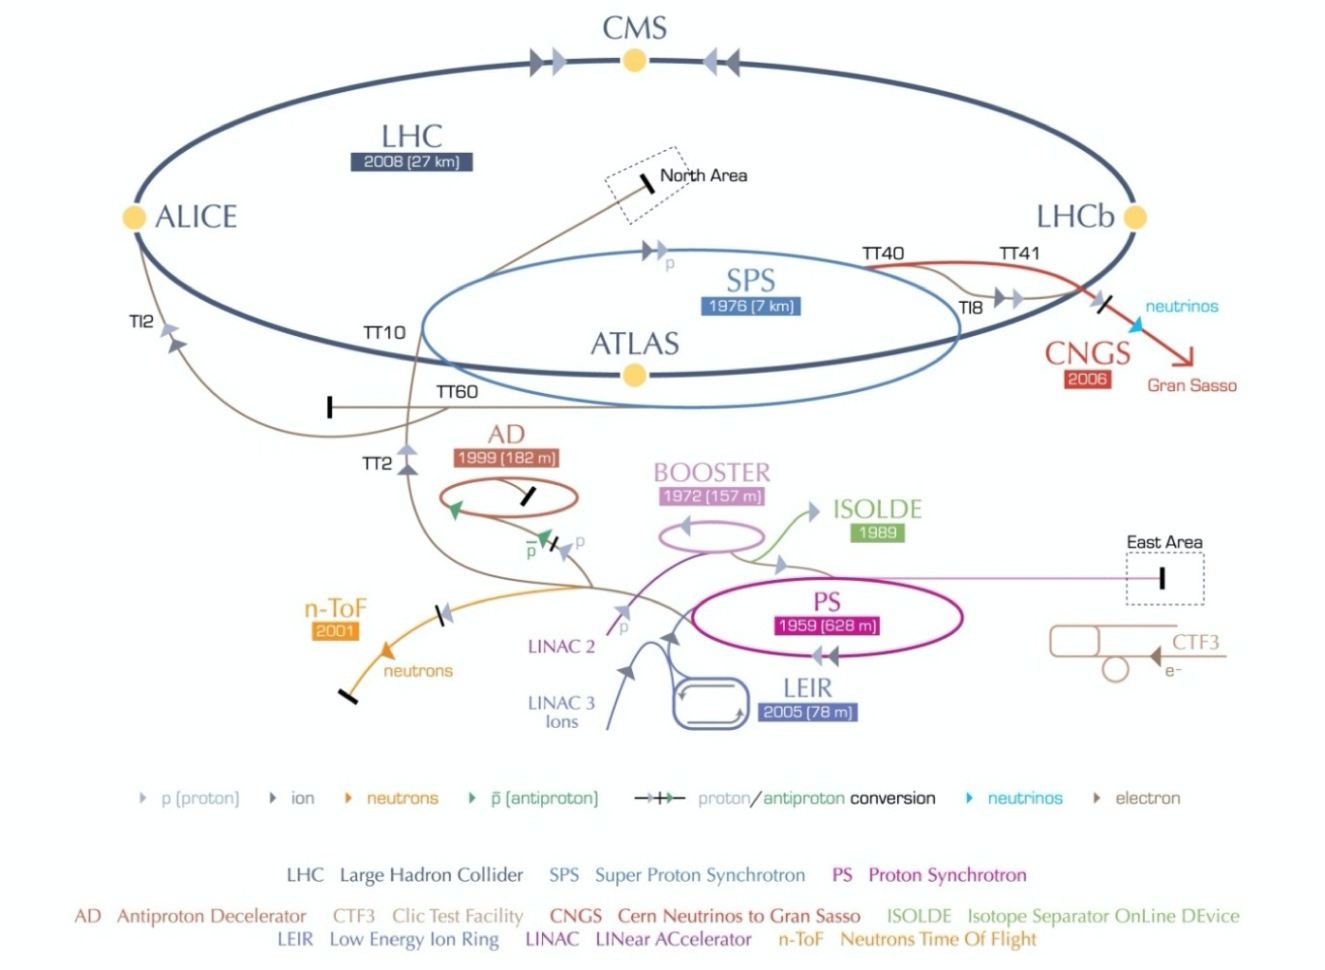
\includegraphics[width=12cm]{LHC_overview}
\caption[LHCの全体像]{LHCの全体像\cite{1-1}}
\label{LHC_overview}
\end{figure}

\section{ATLAS実験}
初めにATLAS実験に用いる座標系と用語について説明する。まず衝突点を原点として定義しており、ビーム軸を$z$軸、これに対して垂直な平面を$x-y$平面とする。
$x$軸方向は原点からみてLHCリングの中心に向かう方向であり、$y$軸は地上に向かう方向である。
方位角$\phi$は$z$軸周りの角度であり、極角$\theta$は$z$軸とのなす角である。大抵、極角$\theta$は以下のようにローレンツ不変量$\eta$で表される。
\bbb
\eta = -\rm{ln tan\left(\frac{\theta}{2}\right)}
\eee


\subsection{ATLAS検出器}
ATLAS検出器は複数の検出器から構成され、陽子の衝突によって生成された粒子の運動量、エネルギーを測定することができる。
最内装に内部飛跡検出器が設置されていて、次に超電導ソレノイド磁石、カロリメータ、トレノイド磁石、ミューオン検出器の順に設置されている。ビームパイプ以外をほとんど検出器で覆うようなデザインとなっている。
ATLAS検出器の全体図を図\ref{atlas_detector}に示す。

\begin{figure}[bpt]\centering
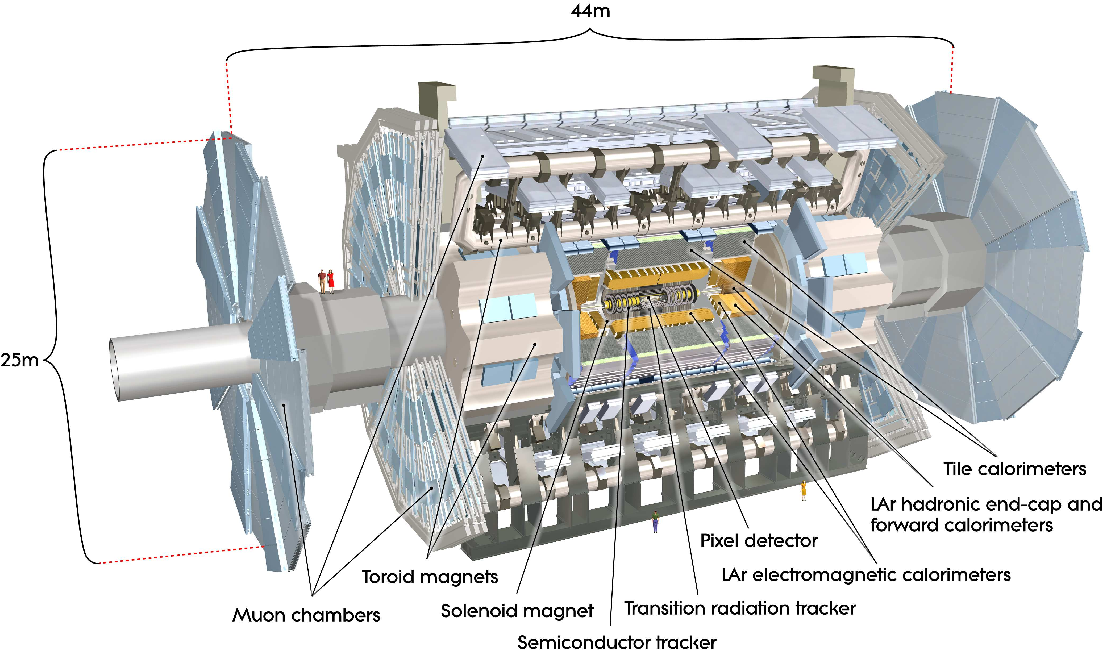
\includegraphics[width=10cm]{atlas_detector}
\caption[ATLAS検出器]{ATLAS検出器\cite{1-2}}
\label{atlas_detector}
\end{figure}

%\begin{figure}[bpt]\centering
%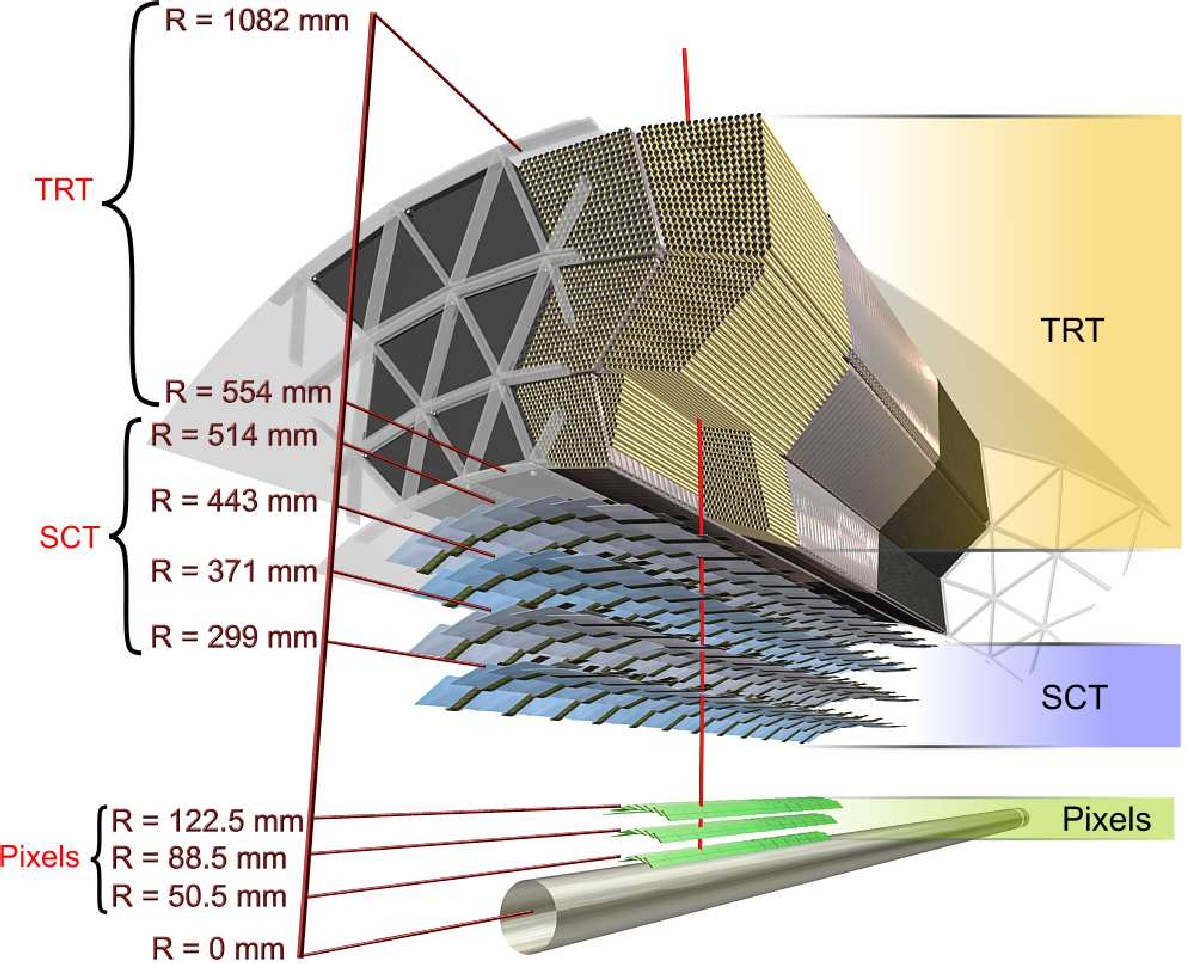
\includegraphics[width=10cm]{atlas_detector_cross_section}
%\caption[ATLAS検出器]{ATLAS検出器\cite{1-2}}
%\label{atlas_detector_cross_section}
%\end{figure}

\subsection{内部飛跡検出器}
ATLAS検出器の最内層に位置する検出器である。
内部飛跡検出器は粒子の飛跡を測定するための検出器であり、その曲がり具合から粒子の運動量を計算できる。
半径$1.15 \rm{m}$、長さ$7 \rm{m}$の円柱形であり、$|\eta|\leq 2.5$の領域を覆っている。超伝導ソレノイド磁石で2 $\rm{T}$の磁場が$z$方向にかけられる。この検出器はさらに3つの検出器で構成され、内側からピクセル検出器、ストリップ検出器、遷移放射検出器の順に設置されている。
ピクセル、ストリップ検出器は階層構造になっており、粒子は複数の検出器を通過する。通過位置をつなぎ合わせることで粒子の軌跡を計算することができる。

内部飛跡検出器の全体図を図\ref{inner_detector}に示す。

\begin{figure}[bpt]\centering
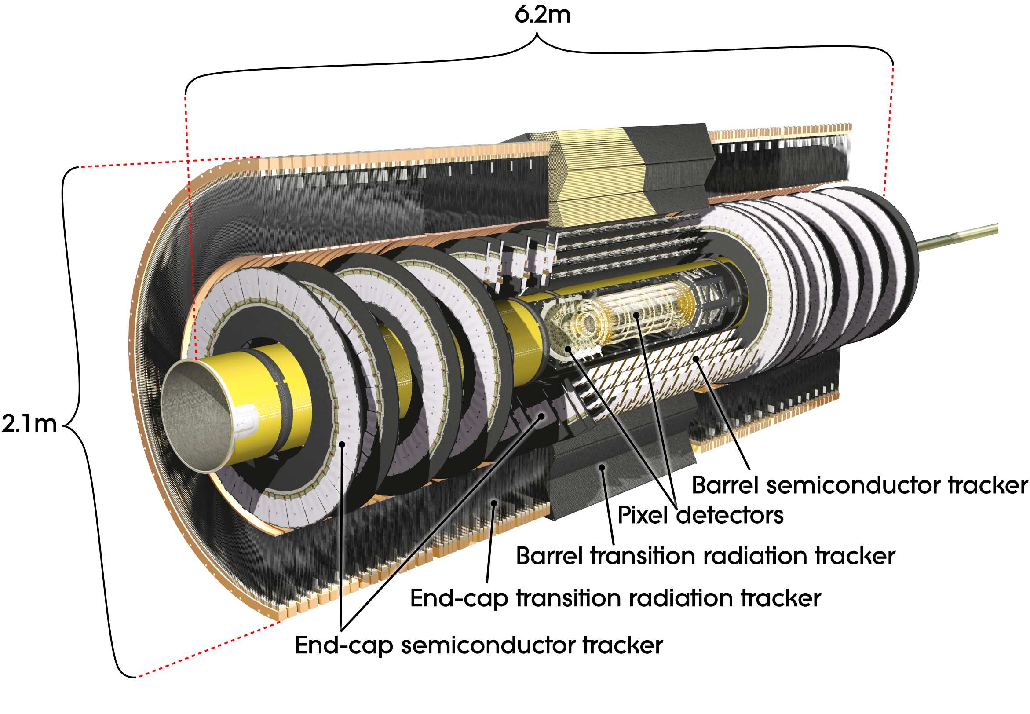
\includegraphics[width=10cm]{inner_detector}
\caption[内部飛跡検出器]{内部飛跡検出器\cite{1-2}}
\label{inner_detector}
\end{figure}


%検出器は$\eta$の範囲によってバレル部とエンドキャップ部に分かれる。図\ref{inner_cross_section}にビーム軸方向の端面図を示す。
%
%\begin{figure}[bpt]\centering
%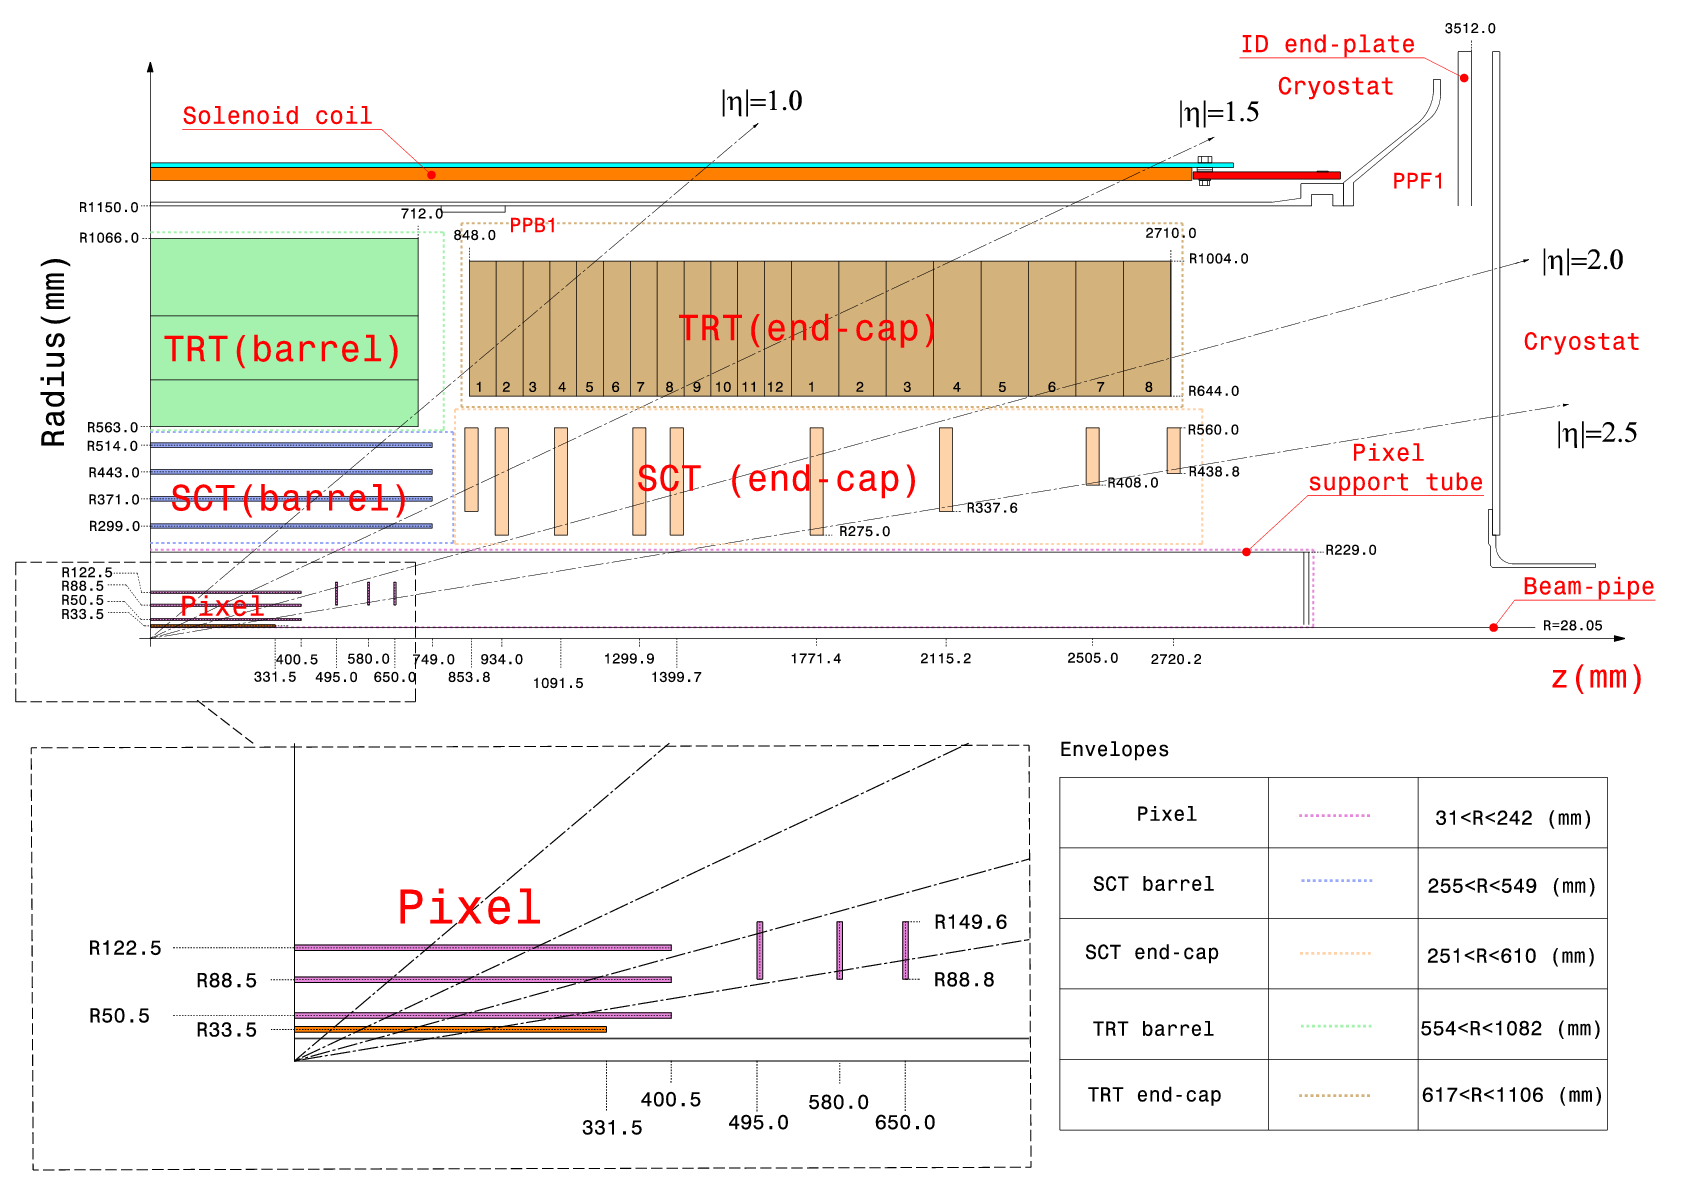
\includegraphics[width=12cm]{inner_cross_section}
%\caption[内部飛跡検出器]{内部飛跡検出器\cite{1-4}}
%\label{inner_cross_section}
%\end{figure}

\clearpage
\subsubsection{ピクセル検出器}

内部飛跡検出器の最内層に位置する検出器である。
ピクセル検出器はバレル層が4層、Diskと呼ばれるエンドキャップ層が6層で構成される。
バレル部の最内層はIBL(Insertable B-Layer)と呼ばれ、順にB-Layer、Layer-1、Layer-2となっている。

ピクセル検出器の全体図を図\ref{pixel_detector_overview}に示す。
\begin{figure}[bpt]\centering
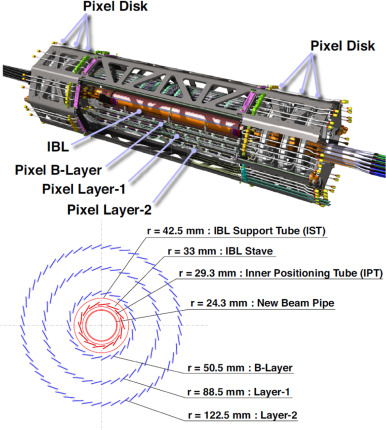
\includegraphics[width=10cm]{pixel_detector_overview}
\caption[ピクセル検出器全体]{ピクセル検出器全体\cite{1-5}}
\label{pixel_detector_overview}
\end{figure}

ピクセル検出器の各層は、モジュールと呼ばれる最小単位の検出器をいくつも搭載している。
ピクセルモジュールを図\ref{pixel_detector}に示す。
このピクセルモジュールの詳細については2章で述べる。
\begin{figure}[bpt]\centering
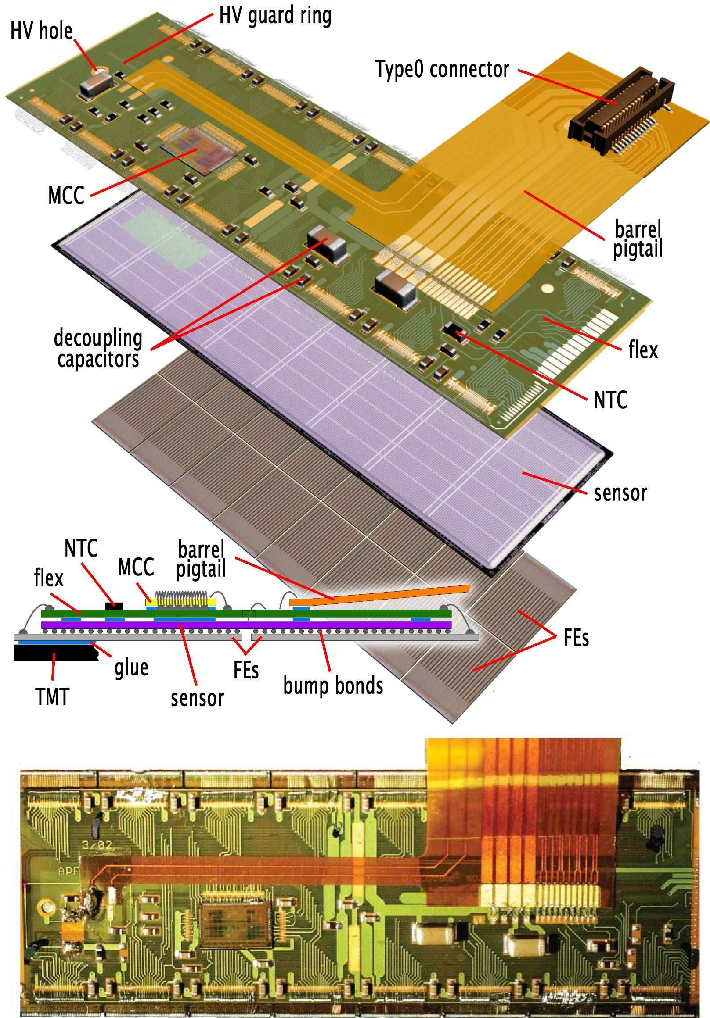
\includegraphics[width=8cm]{pixel_detector}
\caption[ピクセルモジュール]{ピクセルモジュール\cite{1-2}}
\label{pixel_detector}
\end{figure}


\clearpage
\section{HL-LHC実験アップグレード計画}
上述したように、LHCでは加速器のアップグレードを予定しており、これをHL-LHCアップグレード計画と呼ぶ。詳細を以下に示す。
\subsection{概要}
HL-LHCではルミノシティ呼ばれる陽子バンチの密度を上げることで、衝突確率を大きくし、取得統計数を増やす目的がある。
LHCとHL$-$LHCの比較を表\ref{compare_lhc}に示す。

\begin{table}[tbp]
\begin{center}
\caption[LHCの比較]{LHCの比較\cite{1-6}}
\label{compare_lhc}
  \begin{tabular}{|lll|} \hline
    & LHC & HL$-$LHC \\ \hline
    重心系エネルギー & 14 & 14 \\
    瞬間ルミノシティ[$\rm{cm^{-2}s^{-1}}$] & $1\times 10^{34}$ & $7\times10^{34}$ \\
    積分ルミノシティ[$\rm{fb^{-1}}$] & $300$ & $3,000$ \\
    1衝突あたりのイベント数 & $23$ & $138$ \\ \hline 
  \end{tabular}
\end{center}
\end{table}

LHCの運転計画を表\ref{hllhc_plan}に示す。
2020年8月地点の計画では、2025年の初めよりHL-LHCの導入が始まり、2027年の途中からHL-LHC運転開始の予定となっている。
\begin{figure}[bpt]\centering
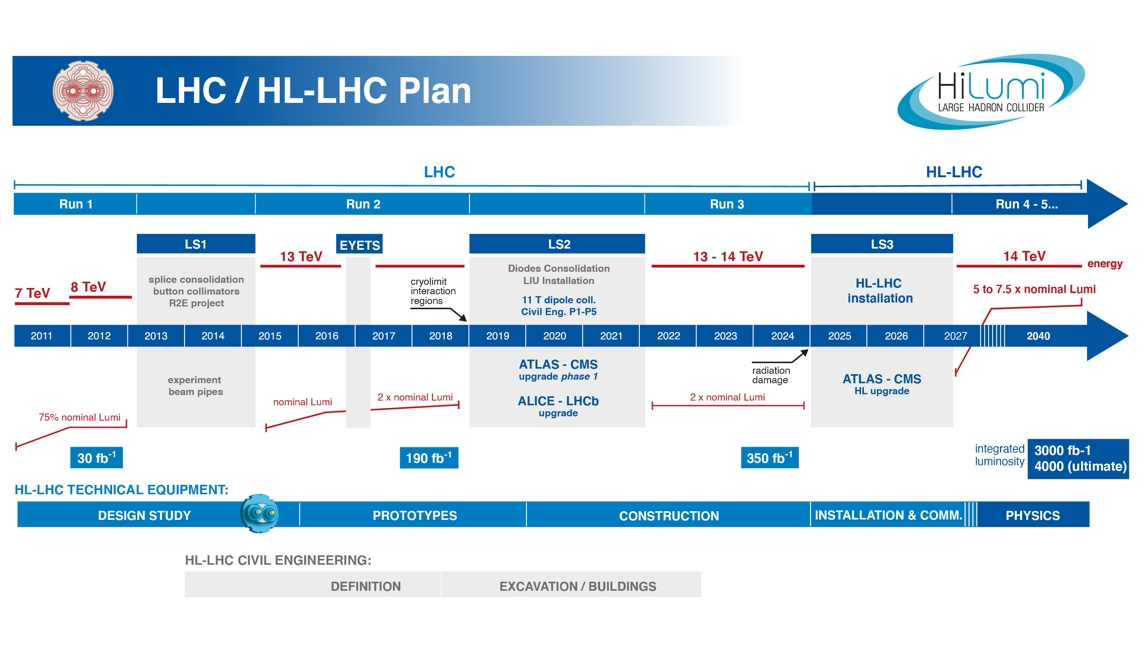
\includegraphics[width=12cm]{hllhc_plan}
\caption[HL-LHC運転計画]{HL-LHC運転計画\cite{1-7}}
\label{hllhc_plan}
\end{figure}

\subsection{内部飛跡検出器のアップグレード}
ルミノシティの増加に伴い、検出器には以下のような性能が要求される。
\begin{itemize}
  \item 放射線耐性の向上
  \item 高速読み出し
  \item 検出器の細密化
\end{itemize}

HL-LHCに向けてATLAS内部飛跡検出器はアップグレードを予定しており、上記の要求を満たすように開発を進めている。
アップグレード後の検出器をITk(Inner Tracker)と呼ぶ。イメージを図\ref{itk_image}に示す。

\begin{figure}[bpt]\centering
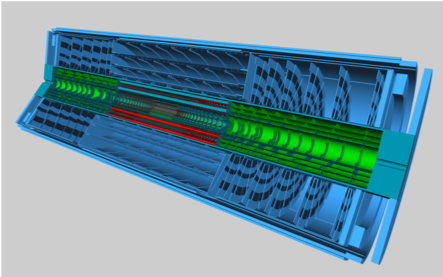
\includegraphics[width=10cm]{itk_image}
\caption[ITkのイメージ]{ITkのイメージ\cite{1-3}}
\label{itk_image}
\end{figure}

\clearpage
\subsubsection{ITkの構成と現行との比較}
図\ref{itk_cross_section}にITkのビーム軸方向の断面図を示す。
ITkはピクセル検出器とストリップ検出器で構成される。
ピクセル検出器はバレル、インクラインド、エンドキャップ部で構成され、バレル部は5層となっている。

\begin{figure}[bpt]\centering
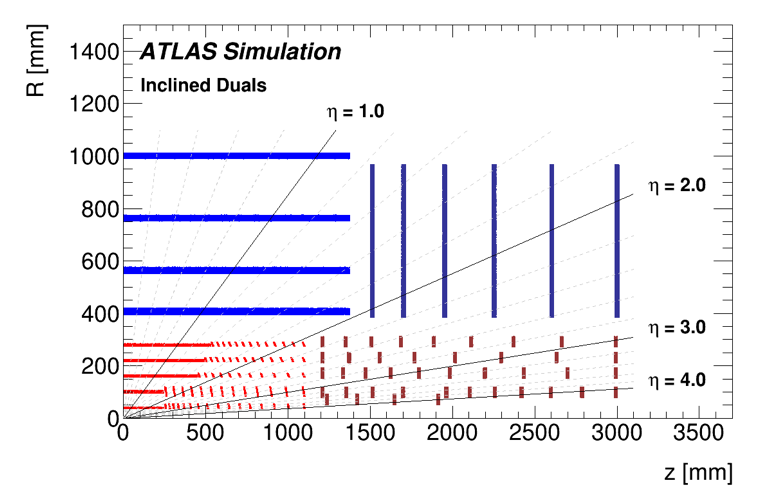
\includegraphics[width=10cm]{itk_cross_section}
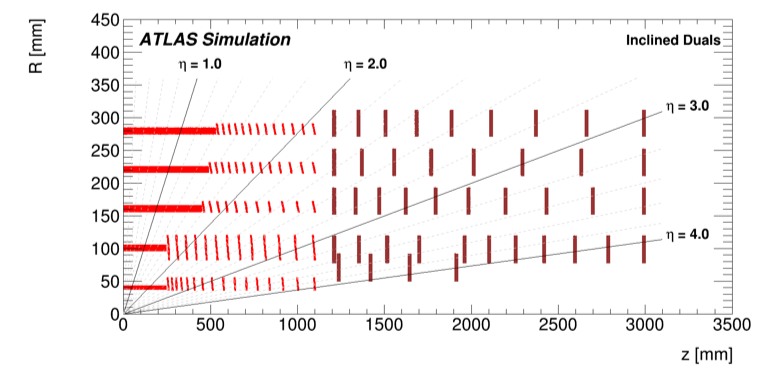
\includegraphics[width=10cm]{itk_pixel_cross_section}
\caption[ITkの断面図]{ITkの断面図\cite{1-3}}
\label{itk_cross_section}
\end{figure}

ピクセル検出器の配置に関して、現行とITkの比較を表\ref{compare_itk_pixel}に示す。
またモジュール数の比較を表\ref{compare_itk_modules}に示す。

\begin{table}[tbp]
\begin{center}
\caption[ピクセル検出器配置の比較]{ピクセル検出器配置の比較}
\label{compare_itk_pixel}
  \begin{tabular}{|lll|} \hline
    & 現行 & ITk \\ \hline
    $r[\rm{mm}]$ & $33~129$ & $39~279$ \\ 
    $|\eta|$ & $<2.5$ & $<4$ \\ 
    層の数 & 4 & 5 \\ \hline
  \end{tabular}
\end{center}
\end{table}

\begin{table}[tbp]
\begin{center}
\caption[ピクセルモジュール数の比較]{ピクセルモジュール数の比較}
\label{compare_itk_modules}
  \begin{tabular}{|l||ll|ll|ll|} \hline
          & バレル部 &            & インクラインド部 & & エンドキャップ部 & \\ \hline 
    層    & 現行     & ITk        & 現行& ITk          & 現行  & ITk \\ \hline
    1     & $280$    & $192$      & $-$ & $512$        & $-$   & $64$ \\ 
    2     & $286$    & $240$      & $-$ & $520$        & $-$   & $242$ \\ 
    3     & $494$    & $660$      & $-$ & $660$        & $-$   & $320$ \\ 
    4     & $676$    & $960$      & $-$ & $1040$       & $288$ & $352$ \\ 
    5     & $-$      & $1300$     & $-$ & $1300$       & $-$   & $468$ \\ \hline
    合計  & $1736$   & $3352$     & $0$ & $4032$       & $288$ & $1446$ \\ \hline\hline
  \end{tabular}
\end{center}
\end{table}

\subsection{期待される物理}
ITkは現行ピクセル検出器に比べカバーする$\eta$の範囲が大きい。
そのため前方方向に大きな運動量を持つ粒子が生じるような物理現象に対する感度が向上する。

このような物理現象の例として、ボゾン粒子結合によるヒッグス粒子生成過程(Vector boson fusion higgs production, \textbf{VBF})をあげる。
この過程のファインマン図及びイベントディスプレイを図\ref{VBF_image}に示す。
この衝突により生じる2つのクオークジェットは前方方向に大きい運動量を持つ。
ITkではこれらのジェットを正確に捉えることができ、VBFイベントの測定精度を向上することができる。
この測定における系統誤差は表\ref{VBF_uncertainty}のように見積もられる\cite{1-3}。

\begin{figure}[bpt]
  \begin{minipage}{0.4\hsize}
    \begin{center}
    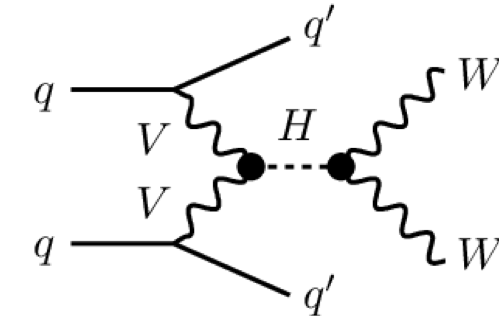
\includegraphics[width=60mm]{VBF_fainman}
    \end{center}
  \end{minipage}
  \begin{minipage}{0.4\hsize}
    \begin{center}
    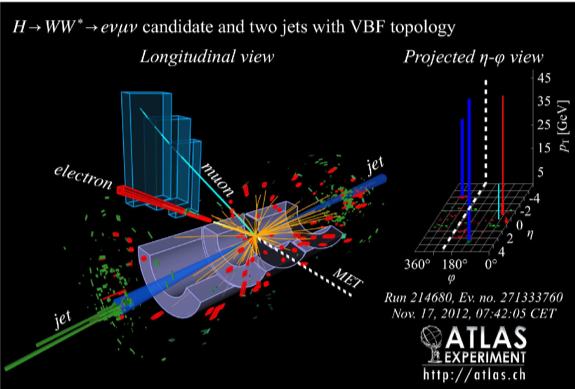
\includegraphics[width=60mm]{VBF_event_display}
    \end{center}
  \end{minipage}
  \caption[VBFイベントの図]{VBFイベントの図}
  \label{VBF_image}
\end{figure}

\begin{table}[tbp]
\begin{center}
\caption[VBFの測定における系統誤差の見積もり]{VBFの測定における系統誤差の見積もり}
\label{compare_itk_pixel}
  \begin{tabular}{|lll|} \hline
    使用範囲 & $|\eta| <2.7 $ & $|\eta| < 4.0 $ \\ \hline
    & 22$\%$ & 12$\%$ \\ \hline
  \end{tabular}
\end{center}
\end{table}

その他広い$\eta$による利点として、bタグ精度の向上、主崩壊イベント由来のジェットの選別精度の向上、$\tau$レプトン識別精度の向上が見込まれ、多くの物理現象において測定精度の向上が見込まれている。

\chapter{ピクセルモジュール}
この章ではピクセルモジュールの構成と各構成部品について説明する。

\section{ピクセルモジュールの構造}
ピクセルモジュールはベアモジュールとフレキシブル基板より構成される。
ベアモジュールは荷電粒子の通過信号を発生するシリコンセンサーと、AD変換を行うFEチップで構成される。
ベアモジュールが持つFEチップの数はモジュールの種類によって異なる。
モジュールの構成を図\ref{module_configuration}に示す。

\begin{figure}[bpt]\centering
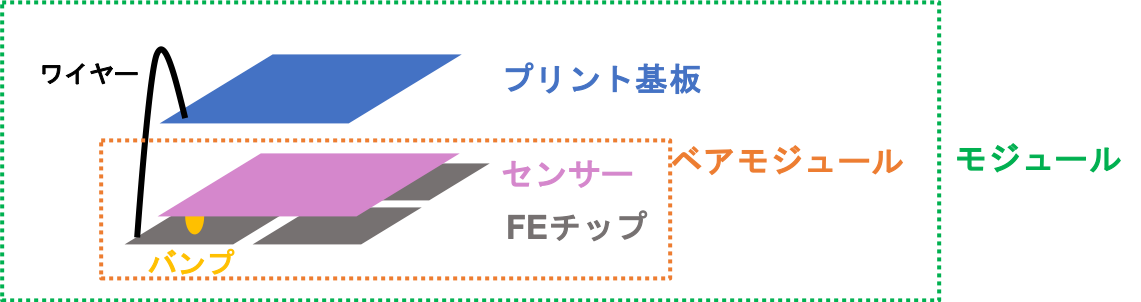
\includegraphics[width=14cm]{module_configuration}
\caption[ピクセルモジュールの構成]{ピクセルモジュールの構成。図はQuadモジュールの構成を模式的に表したものである。モジュールはベアモジュールと呼ばれる構造とフレキシブル基板を貼り付けることで作られる。ベアモジュールはセンサーとFEチップを持ち、Quadモジュールの場合FEチップは4枚である。センサーとFEチップはバンプと呼ばれる構造で電気的に接続しており、1ピクセルに対して1つのバンプ接合がなされている。FEチップとフレキシブル基板の接続には、ワイヤーが複数本配線される。}
\label{module_configuration}
\end{figure}

\section{ピクセルモジュールの構成部品}
\subsection{シリコンセンサー}
ピクセルモジュールに搭載するセンサーはシリコン半導体を用いている。
センサー内部にはpn接合\cite{2-1}を持つ。センサーに逆バイアス電極をかけ、空乏層\cite{2-1}を広げた状態で用いる。
この空乏層領域に荷電粒子が通過すると、Bethe-Blochの式\cite{2-1}に従い粒子はエネルギーを損失する。
このエネルギー損失量に従い、電子・ホール対が生成、これを収集することで荷電粒子の通過信号をアナログ信号として読み出すことができる。

新型ピクセルモジュールに搭載するセンサーは、n${}^+$ - in - p型である。
模式図を図\ref{sensor_image}に示す。$n^+$電極で電子を収集し、信号取得を行う。
現行のセンサーに比べ、型変換を起こす可能性がなくなり安定した運転が見込まれる。\cite{1-3}

\begin{figure}[bpt]\centering
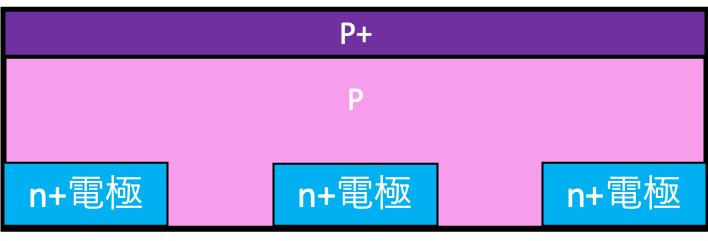
\includegraphics[width=8cm]{sensor_image}
\caption[新型ピクセルモジュールに搭載するシリコンセンサー]{新型ピクセルモジュールに搭載するシリコンセンサー。図は新型ピクセルモジュールに搭載するシリコンセンサーの模式図を示している。n${}^+$ - in - p型と呼ばれるp型半導体にn${}^+$型電極を埋め込んだ構造を持ち、逆バイアス電圧を印加するとn${}^+$側から空乏層が広がる。}
\label{sensor_image}
\end{figure}

\subsection{読み出しFEチップ}
読み出しFEチップはシリコン半導体を用いて作られた集積回路である。
読み出しFEチップの主な役割は、シリコンセンサーで発生し受け取ったアナログ信号を整形、増幅したのちAD変換し、後段に転送することである。
AD変換について、アナログ信号がThresholdを超えた時間幅を測定し、デジタル信号に変換する。この信号の値を\textbf{Time over Threshold(ToT)}と呼ぶ。

このAD変換の流れのイメージを図\ref{tot_algorithm}に示す。

\begin{figure}[bpt]\centering
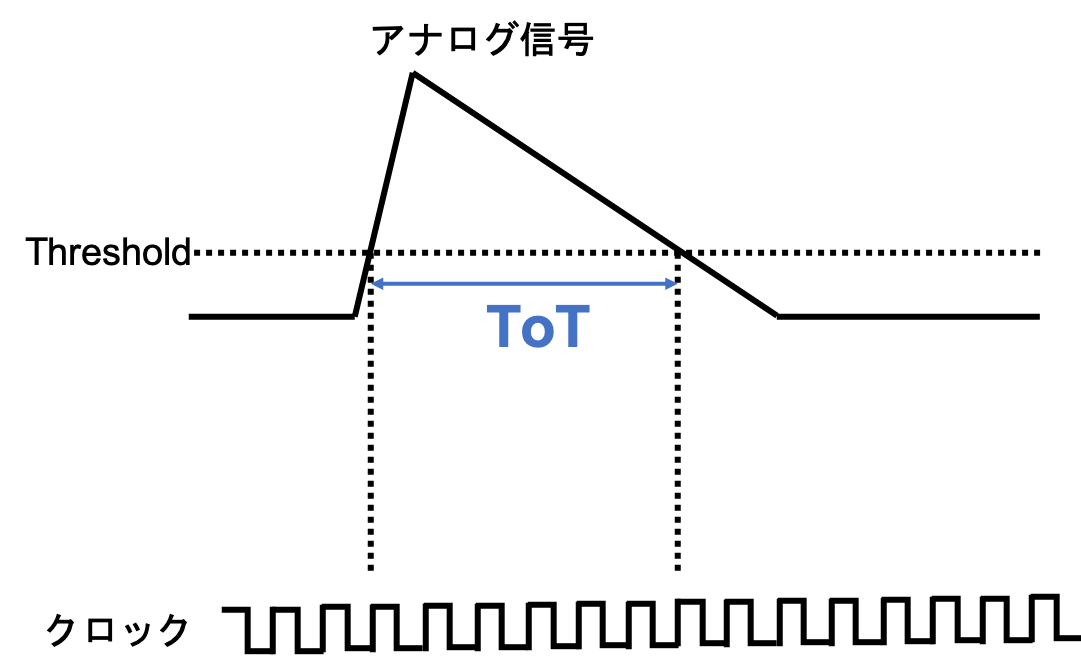
\includegraphics[width=10cm]{tot_algorithm}
\caption[ToTの概念図]{ToTの概念図。FEチップで生成されるデジタル信号はToTと呼ばれる。図はその概念を模式的に表したものであり、FEチップで行われているAD変換である。ToTはアナログ信号がThreshold値を超えた時間幅に相当する。実際にはToT間のクロック数[b.c.]として取得され、1b.c.(25~ns)はLHCにおける陽子の衝突間隔に相当する。}
\label{tot_algorithm}
\end{figure}



\subsubsection{RD53A}
RD53A\cite{2-1}は、新型ピクセルモジュールの研究、開発のために作られたプロトタイプの読み出しFEチップである。
RD53Aの性能を表\ref{rd53a_spec}に示す。
チップサイズ、ピクセル数はITkに搭載するモジュールの半分となっている。

\begin{table}[tbp]
\begin{center}
\caption[RD53Aの性能]{RD53Aの性能。}
\label{rd53a_spec}
  \begin{tabular}{|ll|} \hline
    チップサイズ[mm$^2$] & $20.0\times 11.6$ \\ 
    ピクセルサイズ[$\mu$m$^2$] & $50.0\times 50.0$ \\ 
    ピクセル数[行$\times$列] & $400\times 192$ \\ 
    トリガーレート[kHz] & $1000$ \\ 
    データレート[Mbps] & $1280\times4$ \\ \hline
  \end{tabular}
\end{center}
\end{table}

FEチップ上の各ピクセルはアナログ回路部とデジタル回路部を持つ。
RD53Aでは図\ref{fechip_rd53a}に示すように、3つの領域があり、それぞれの領域でピクセルのアナログ回路、AD変換回路が異なる。
左から順にSynchronous FE、Linear FE、Differrential FEと呼ぶ。
研究開発用に3つの領域が設けられており、ITkに搭載するモジュールにはDifferrentialフロントエンドを用いることが決定している。
なお、デジタル回路部は全てのピクセルにおいて共通である。
それぞれの回路図を付録\ref{chap:rd53a_circit}に示す。

\begin{figure}[bpt]\centering
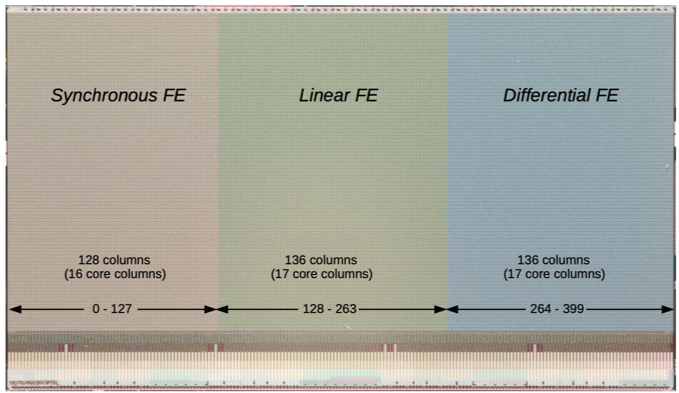
\includegraphics[width=10cm]{fechip_rd53a}
\caption[RD53A]{RD53A\cite{2-1}。ピクセル数は400列$\times$192行となっている。図のようにRD53Aは3つの領域が設けられており、それぞれSynchronous FE、Linear FE、Differential FEと呼ぶ。各領域のピクセルが持つアナログ回路、AD変換回路が異なる設計となっている。}
\label{fechip_rd53a}
\end{figure}

\subsection{フレキシブル基板}
フレキシブル基板は、基板上に電子部品が搭載されたものである。
FEチップからのデジタル信号を後段の回路へ転送する他、FEチップ、センサーへの電圧印加制御の役割も担う。

\subsection{信号伝達}
モジュールの信号伝達の様子を模式的に表したものを図\ref{module_electric_overview}に示す。

\begin{figure}[bpt]\centering
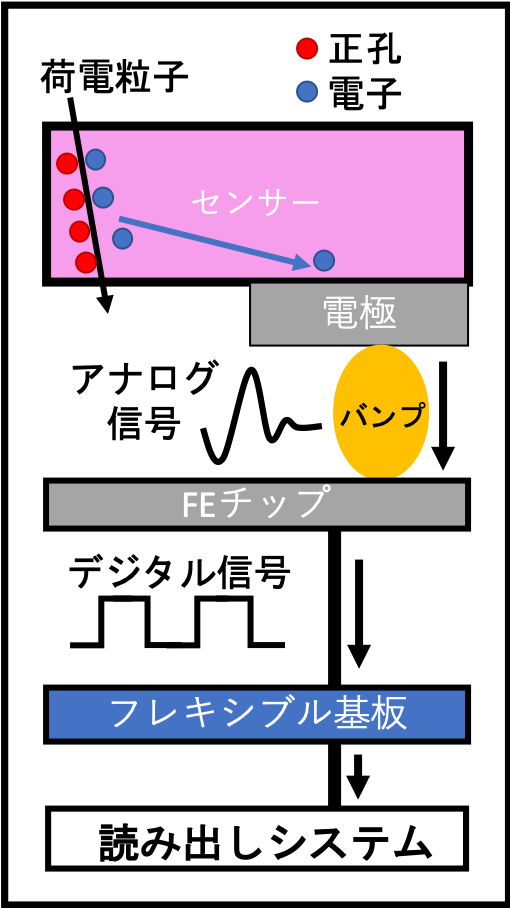
\includegraphics[width=6cm]{module_electric_overview}
\caption[ピクセルモジュールにおける信号伝達の様子]{ピクセルモジュールにおける信号伝達の様子。図はピクセルモジュールにおける信号伝達の様子を模式的に表したものである。初めに、荷電粒子がセンサー部を通過し、エネルギー損失に応じた電子・ホール対を生成する。電子は電極により収集され、バンプを通してアナログ信号としてFEチップに送られる。FEチップでは信号を整形、増幅後、デジタル信号に変換する。その後ワイヤーを通してフレキシブル基板に転送、そしてPCに転送されデータを取得する。}
\label{module_electric_overview}
\end{figure}

\section{新型モジュールの種類}
現在、ITkに搭載するモジュールとして以下の3つのモジュールを予定している。
\begin{itemize}
  \item ステーブ用Tripletモジュール
  \item リング用Tripletモジュール
  \item Quadモジュール
\end{itemize}

Triplet、QuadモジュールはそれぞれFEチップを3、4枚搭載するモジュールである。
それぞれのモジュールの図及び検出器上における位置の一例を図\ref{module_geom}に示す。


\chapter{モジュール組み立てと品質試験} \label{chap:qc_test}
ITkに搭載するピクセルモジュールは、世界中に存在する複数の組み立て機関で製造される。
またモジュールの組み立てともに性能確認のための品質試験を行う。

本研究の主題はこのモジュール品質試験のデータ管理を行うデータベースシステムの開発である。
本章ではデータ管理の対象となるモジュールの組み立て工程と品質試験の概要を説明する。
開発したデータベースシステムについては\ref{chap:dbsystem}章で説明する。

\section{組み立て工程}\label{sec:assembly}
モジュール組み立て機関は、初めにベアモジュールとフレキシブル基板をそれぞれの製造機関から受け取る。
組み立て工程として以下が設定されている。
\begin{enumerate}
  \item ベアモジュール・フレキシブル基板貼り付け.
  \begin{itemize}
    \item 受け取ったベアモジュールとフレキシブル基板を接着剤を用いて貼り付ける。
  \end{itemize}
  \item ワイヤー配線.
  \begin{itemize}
    \item ワイヤー配線を行い、FEチップとフレキシブル基板を電気的に接続する。
  \end{itemize}
  \item ワイヤー保護.
  \begin{itemize}
    \item ワイヤーが損傷があり断線が起きると、そのワイヤーに接続されているピクセルの読み出しができなくなる。これを防ぐため、モジュールに屋根型の構造を取り付け、ワイヤーを物理的に保護する。
  \end{itemize}
  \item パリレンコーティング.
  \begin{itemize}
    \item モジュール読み出し部以外での電通や放電を防ぐため、パリレン高分子を用いてモジュールを保護する。
  \end{itemize}
  \item 温度サイクル試験.
  \begin{itemize}
    \item ITk運転時の環境温度は$-45^\circ$Cから$40^\circ$Cまで変化しうる\cite{3-2}。この温度変化に耐えうるかを確認するため、温度サイクルを行う。
  \end{itemize}
  \item 低温耐久試験.
  \begin{itemize}
    \item ITk運転時の典型的な環境温度は$-15〜0^\circ$C付近である。これに耐えうる性能を持つかを確認するために、低温下にモジュールを長時間設置する耐久試験を行う。
  \end{itemize}
\end{enumerate}

流れと各組み立て工程のイメージを図\ref{assembly_flow}に示す。
\begin{figure}[bpt]\centering
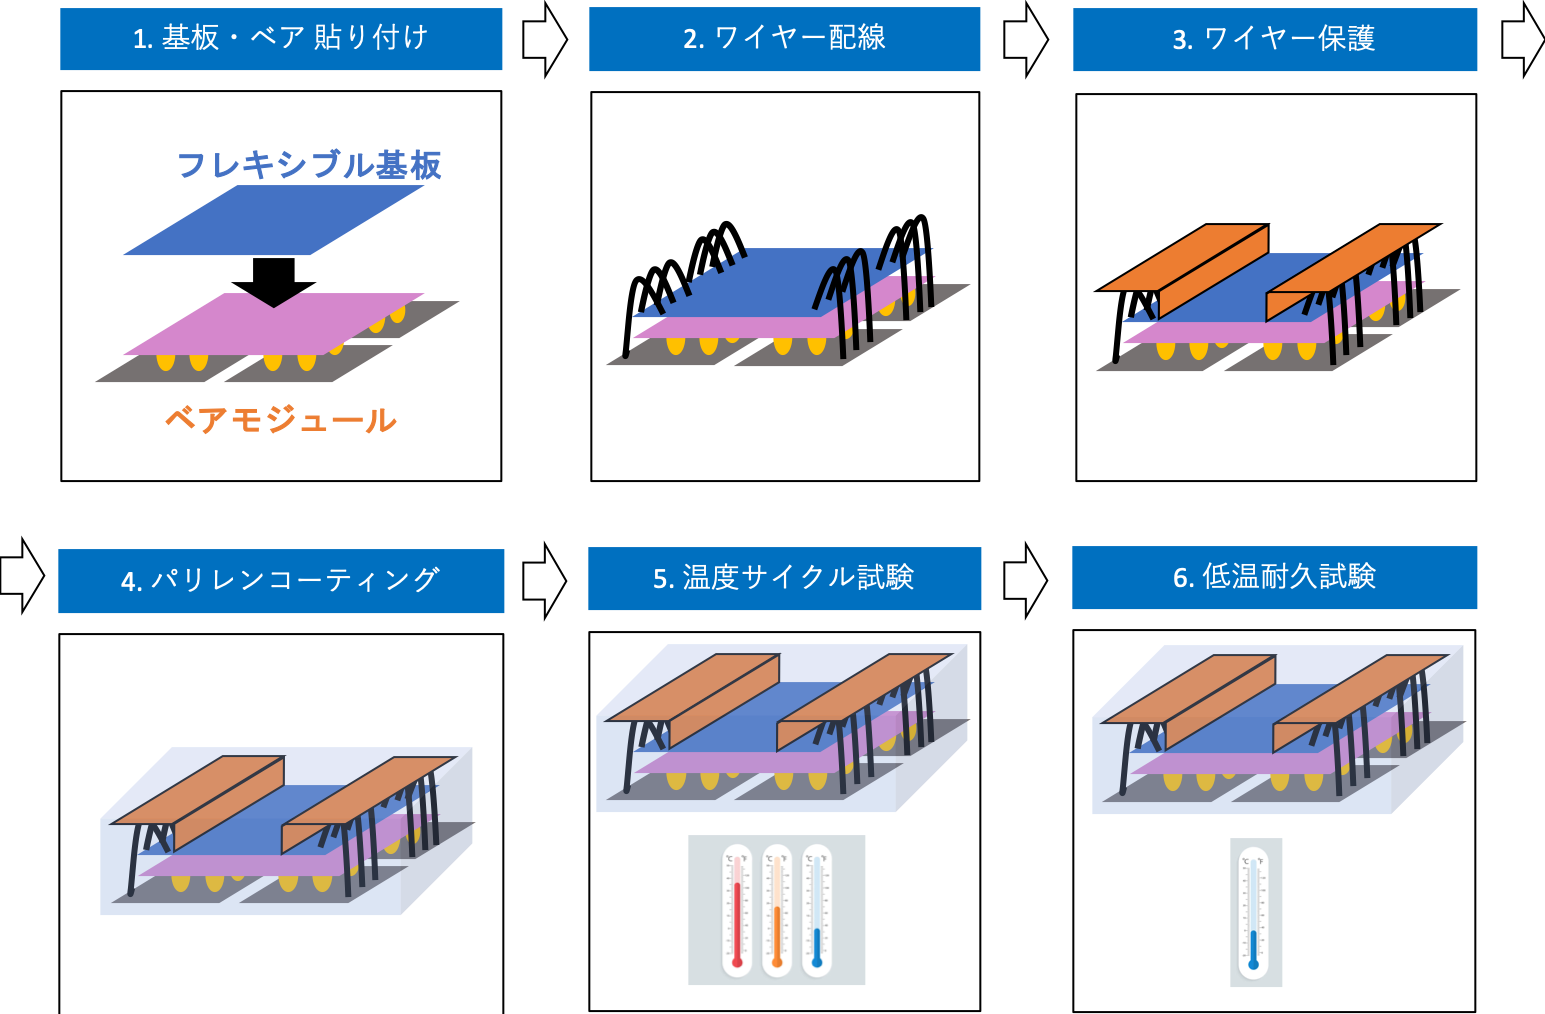
\includegraphics[width=12cm]{./assembly_flow.png}
\caption[組み立て工程のイメージ図]{組み立て工程のイメージ図。モジュール組み立て機関はベアモジュール、フレキシブル基板を受け取り、それらの貼り付け、ワイヤー配線、ワイヤー保護、パリレンコーティング、温度サイクル試験、低温耐久試験の順に組み立てを行う。}
\label{assembly_flow}
\end{figure}

\section{品質試験}
各組み立て工程に対して、いくつかの品質試験を行う。行う品質試験の代表的なものを以下に示す。

\subsection{外観検査}
モジュールの外観写真を撮り、モジュールに以下のような欠陥がないかを確認する。
また外観検査の様子を図\ref{VI_overview}に示す。
\begin{itemize}
  \item 抵抗等取り付け部品の損傷.
  \item ワイヤーの接着位置確認.
  \item 回路やワイヤーの断線.
  \item 付着汚れ.
\end{itemize}

\begin{figure}[bpt]\centering
  \begin{minipage}{0.4\hsize}
    \begin{center}
    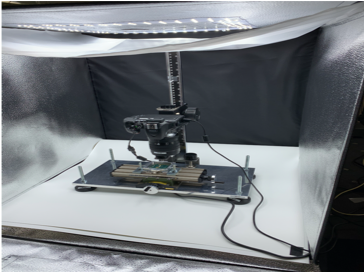
\includegraphics[width=60mm]{./VI_setup.png}
    \end{center}
  \end{minipage}
  \begin{minipage}{0.4\hsize}
    \begin{center}
    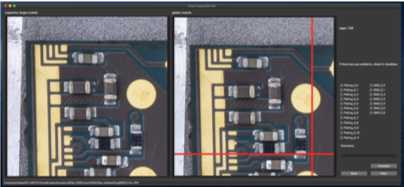
\includegraphics[width=65mm]{./VI_analysis.png}
    \end{center}
  \end{minipage}
  \caption[外観検査の様子]{外観検査の様子。図は日本で実際に行われた外観検査における写真撮影の様子(左図)と撮影写真の確認画面(右図)である。左図のように、写真撮影は光量を制御するため暗箱の中で行っている。写真撮影後、右図のように撮影した写真と良好なモジュールの写真を見比べ、電気部品の損傷、回路の断線などの何らかの所見があった場合には記録をする。}
  \label{VI_overview}
\end{figure}

\subsection{質量測定}
モジュールの質量を測定する試験である。

\subsection{平坦性測定}
モジュール上の位置座標を何点か測定し、モジュールの平坦度、厚さ、歪み具合等を測定する。
測定の様子と解析の例を図\ref{Metrology_overview}に示す。

\begin{figure}[bpt]\centering
  \begin{minipage}{0.4\hsize}
    \begin{center}
    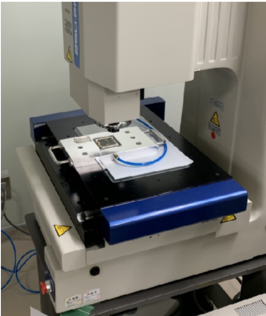
\includegraphics[width=60mm]{./Metrology_setup.png}
    \end{center}
  \end{minipage}
  \begin{minipage}{0.4\hsize}
    \begin{center}
    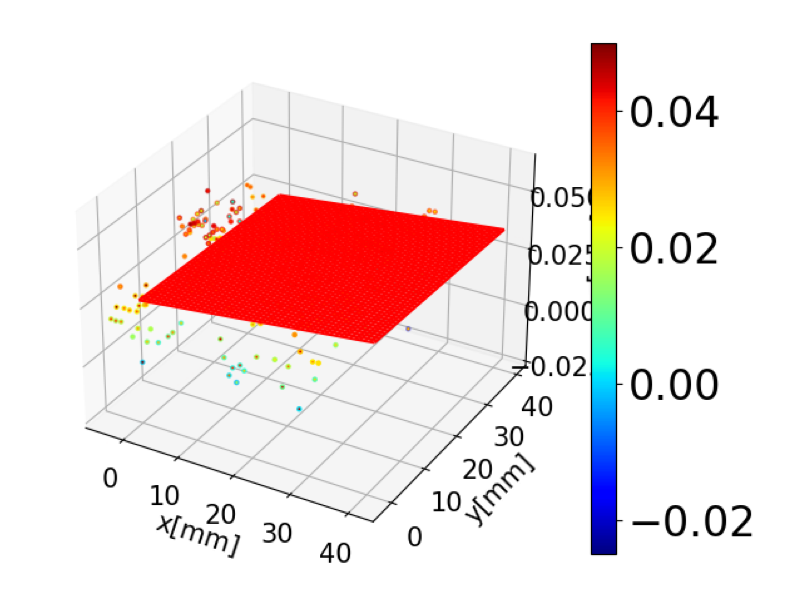
\includegraphics[width=65mm]{./Metrology_analysis.png}
    \end{center}
  \end{minipage}
  \caption[平坦性測定の様子。]{平坦性測定の様子。図は日本で実際に行われた平坦性測定における測定の様子(左図)と解析結果(右図)である。左図のように専用の装置を用いてモジュールの位置座標を何点か測定する。得られた測定点は右図のように図示し、平面でフィッティングを行う。フィット平面からのズレや、モジュールの厚みを計算する。}
  \label{Metrology_overview}
\end{figure}

\clearpage
\subsection{センサー電流-電圧特性確認}
モジュールのシリコンセンサーに逆バイアス電圧をかけ、電流-電圧特性をみる。
印加電圧を段階的に変化させながら電流値を記録し、電圧-電流間の関係を確認する。
この試験の結果の例を図\ref{sensor_IV_result}に示す。
逆方向電圧では電流はほとんど流れないが、降伏電圧に達すると急激に増大する。
これはpn接合の特性\cite{2-1}であり、正常であればこの振る舞いを確認することができる。

\begin{figure}[bpt]\centering
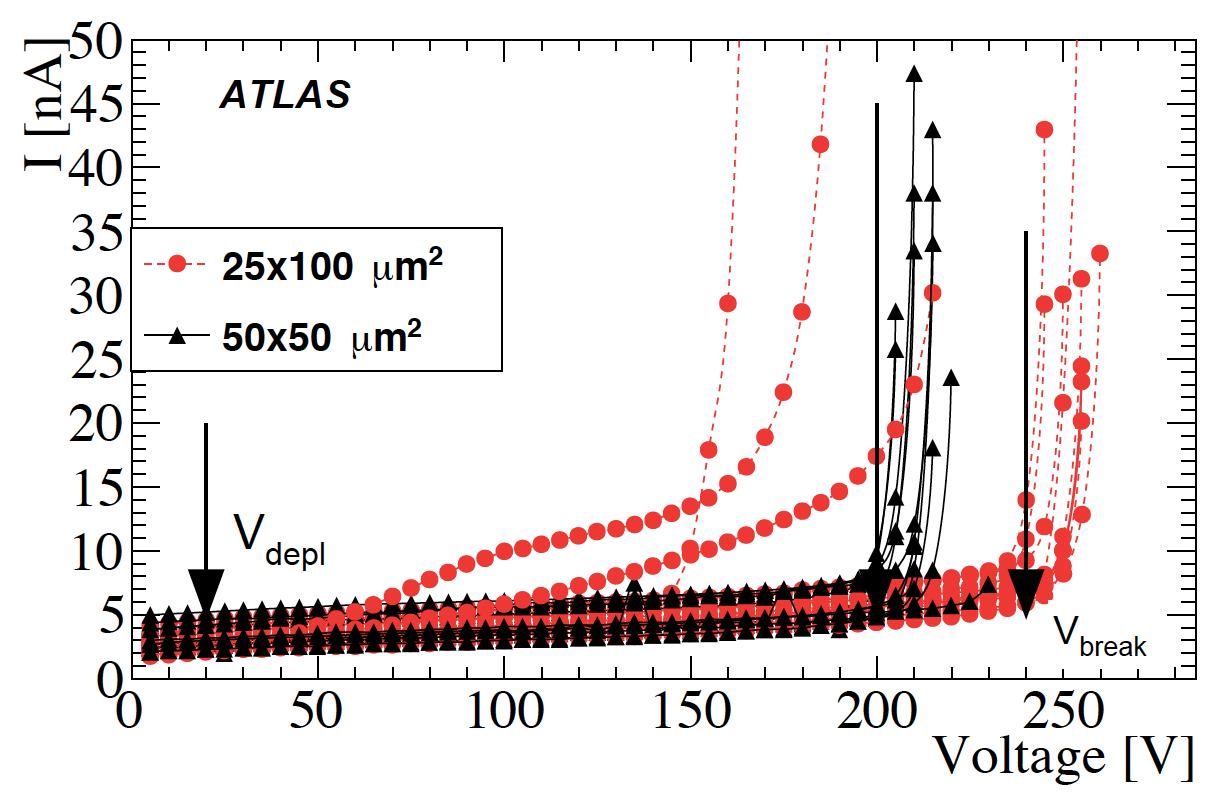
\includegraphics[width=8cm]{./sensor_IV_result.png}
\caption[センサー電流-電圧特性結果の例]{センサー電流-電圧特性結果の例\cite{1-1}。図は複数のセンサーに対する測定結果の例を表している。横軸にセンサーに対する印加電圧[V]、縦軸に電流[nA]を示す。逆バイアス電圧を印加しているため、電流がほとんど流れていないが、ある地点から電流が急激に増加していることが分かる。この降伏電圧はセンサーにより個体差があるが、どれも$150-250$~V付近となっていることが分かる。}
\label{sensor_IV_result}
\end{figure}

\subsection{FEチップ電流-電圧特性確認}
FEチップに対して電圧をかけ、電流-電圧特性をみる。
設定電流を段階的に変化させながら電圧値を記録し、電流-電圧間の関係を確認する。
この試験の結果の例を図\ref{SLDO_VI_result}に示す。
FEチップは抵抗として振る舞い、電流、電圧間の関係は線形性を持つ。

\begin{figure}[bpt]\centering
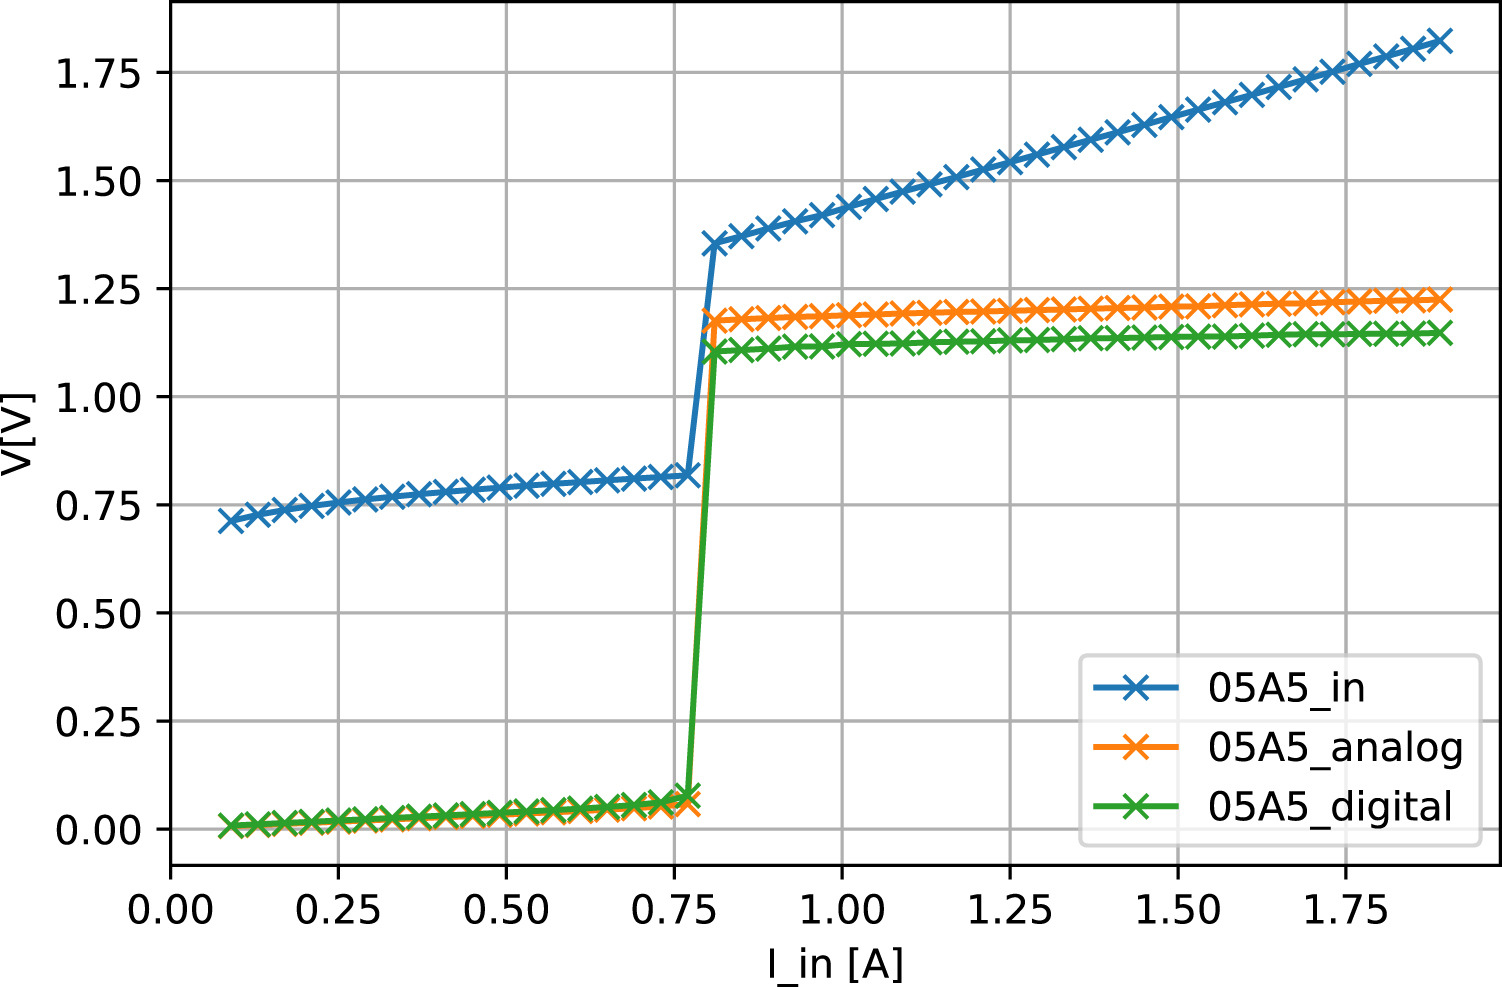
\includegraphics[width=8cm]{./SLDO_VI_result.jpg}
\caption[FEチップ電流-電圧特性試験結果の例。]{FEチップ電流-電圧特性試験結果の例\cite{3-7}。横軸にFEチップに対する設定電流、縦軸は測定した実際にFEチップにかかる電圧値を示している。青、橙、緑はそれぞれ回路全体、アナログ回路部、デジタル回路部に加わる電圧値である。0.75~V付近で急激に電圧が増大しており、この段階でFEチップが機能するようになる。それ以降は線形になっているのが分かる。}
\label{SLDO_VI_result}
\end{figure}

\clearpage
\subsection{読み出し試験}
読み出し試験では、読み出し回路が正常に機能するのかを確認する。
読み出し試験の様子を図\ref{readout_overview}に示す。モジュールに読み出しケーブルを配線し、PCと通信を行い、データを取得する。
また試験において温度、FEチップやセンサーに与える電圧、電流といった検出器の操作、環境関わる情報取得を同時に行い、異常がないかを確認する。これらの情報は「\textbf{Detector Control System, DCS}」と呼ぶ。

\begin{figure}[bpt]\centering
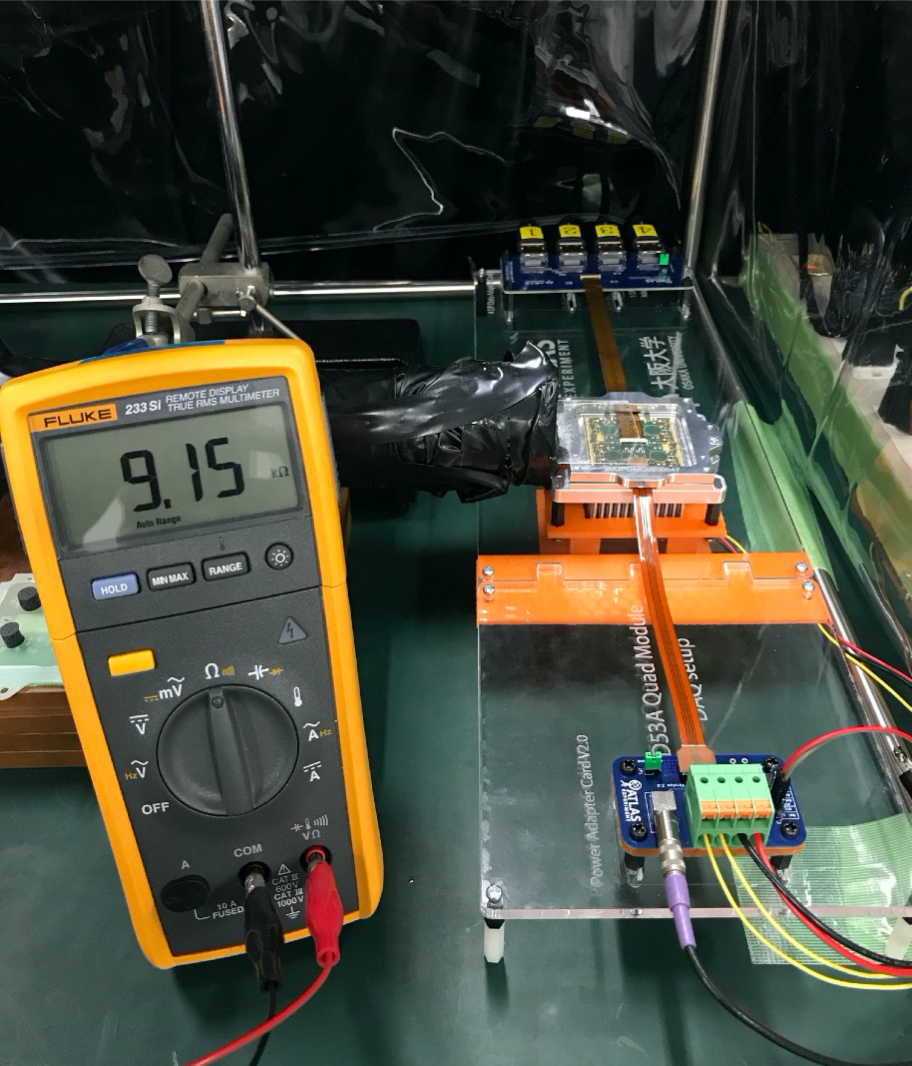
\includegraphics[width=7cm]{./readout_overview.png}
\caption[読み出し試験の様子]{読み出し試験の様子。図は日本で実際に行われた読み出し試験の様子である。図の右側に見えるように、モジュールにケーブルを配線し、PCとの通信を行うことでデータ取得をする。また図の左側では抵抗値を測定している。これはモジュールに付属しているサーミスタの抵抗値を確認することで、温度情報を取得するためのものである。}
\label{readout_overview}
\end{figure}

\subsubsection{汎用読み出しシステムYARR}
\textbf{YARR(Yet Another Rapid Readout)}システム\cite{3-3}は、ピクセルモジュール用に開発された、PCI Express(PCIe)接続を用いた読み出しシステムである。
ファームウェア、ソフトウェアから構成される。YARRではファームウェア上で行う処理はデータ通信やトリガー処理等の最低限に抑え、その他多くの処理をソフトウェアで担うという特徴がある。

\clearpage
\subsubsection{読み出し試験に使用するファイルと変数}
YARRで扱う全てのファイルは\textbf{JSON(JavaScript Object Notation)}と呼ばれる形式で記述される。

YARRを用いた読み出し試験では以下の設定ファイルが要求される。
\begin{itemize}
  \item 試験設定ファイル.
  \begin{itemize}
    \item 読み出し試験の初期設定や解析手法を記述する。
  \end{itemize}
  \item ハードウェア設定ファイル.
  \begin{itemize}
    \item 試験に用いるハードウェアの指定や設定を記述する。
  \end{itemize}
  \item 接続設定ファイル.
  \begin{itemize}
    \item 読み出しを行うFEチップの種類やチャンネルを記述する。
  \end{itemize}  
  \item FEチップ設定ファイル.
  \begin{itemize}
    \item 各FEチップ毎に出力され、全ピクセルに共通な試験の設定値、各ピクセル固有の設定値を記述する。
  \end{itemize}  
\end{itemize}

また試験1項目ごとに以下のファイルが、1つのディレクトリに生成される。
\begin{itemize}
  \item 試験結果ファイル.
  \begin{itemize}
    \item 読み出し試験の結果値を記述する。
  \end{itemize}
  \item 試験設定ファイル.
  \item FEチップ設定ファイル.
  \begin{itemize}
    \item 試験の中で変更が加えられるため、各FEチップにつき試験前後の2つのファイルが出力される。
  \end{itemize}
  \item 試験ログ.
  \begin{itemize}
    \item 試験情報を記録する。
  \end{itemize}
\end{itemize}

後述するローカルデータベースシステムにおいてはさらに以下の設定ファイルを用いる。
\begin{itemize}
  \item データベース設定ファイル.
  \item 試験者設定ファイル. 
  \item 試験場所設定ファイル.
\end{itemize}

読み出し試験項目において以下の$Occupancy$という量が定義される。
試験用電荷の入射数や発行トリガーの数等、発行した信号数を$n_i$回、取得信号数を$n_0$としたとき、
\bbb
\label{occupancy}
Occupancy = \frac{n_0}{n_i} \times 100~[\%]
\eee
と定義する。

読み出し試験では各FEチップに対して「\textbf{レジスタ}」と呼ばれる設定値が存在し、FEチップ上の全ピクセルに対して共通なものを「\textbf{グローバルレジスタ}」、各ピクセル固有のものを「\textbf{ピクセルレジスタ}」と呼ぶ。
レジスタの1つにThreshold用レジスタがある。読み出し試験ではこのレジスタの調整を行う。

\clearpage
\subsubsection{読み出し試験項目}
以下に読み出し試験項目の一覧を示す。
\begin{description}
  \item[レジスタの読み書き.]\mbox{}\\
グローバル及びピクセルレジスタの読み書きが正常にできるのかを確認する試験.
  \item[デジタル回路読み出し.]\mbox{} \\
各ピクセルのデジタル回路部に試験用電荷を入射し、信号の応答数を確認する試験. デジタル回路部の性能確認に用いる.
  \item[アナログ回路読み出し.]\mbox{}\\
各ピクセルのアナログ回路部に試験用電荷を入射し、信号の応答数を確認する試験. アナログ回路部の性能確認に用いる.
  \item[Threshold測定.]\mbox{}\\
各ピクセルのThreshold値を測定する試験.
  \item[Thresholdグローバルレジスタ調整.]\mbox{}\\
Thresholdグローバルレジスタの変更、基準となるThresholdに近づけるための調整.
  \item[Thresholdピクセルレジスタ調整、再調整、精密調整.]\mbox{}\\
Thresholdピクセルレジスタの変更、基準となるThresholdに近づけるための調整.
  \item[ToTグローバルレジスタ調整.]\mbox{}\\
ToTグローバルレジスタの変更、基準となるToTに近づけるための調整.
  \item[ノイズ占有率測定.]\mbox{}\\
各ピクセルのノイズの頻度を確認する試験.
  \item[スタックピクセル測定.]\mbox{}\\
入力電荷の有無にかかわらず、常に信号を出力するピクセルを確認する試験.
  \item[クロストーク測定.]\mbox{}\\
各ピクセルのクロストークの有無を確認する試験. 隣接するAnalog FEに試験用電荷を入射し、応答を確認する.
  \item[バンプ接続確認測定.]\mbox{}\\
各ピクセルのバンプ接合が正常かを確認する試験. 隣接するAnalog FEに大きめの試験用電荷を入射する. バンプが正常であればクロストークにより応答を確認できる.
\end{description}

各試験における試験用電荷入射の方法について、付録\ref{chap:rd53a_circit}に示す。

\clearpage
主な試験項目の詳細について以下で説明する。
\subsubsection{デジタル回路読み出し}
各ピクセルのデジタル回路部に試験用電荷を入射し、信号を取得する。
$Occupancy$(式\ref{occupancy})は、入射電荷数$n_i$と取得信号数$n_0$で定義される。
YARRのデフォルトでは$n_i=100$となっている。

デジタル回路読み出しにおける$Occupancy$の二次元分布の例を図\ref{dig_occ}に示す。
一般にこの試験において、$Occupancy$は100であることが望ましい。

\begin{figure}[bpt]\centering
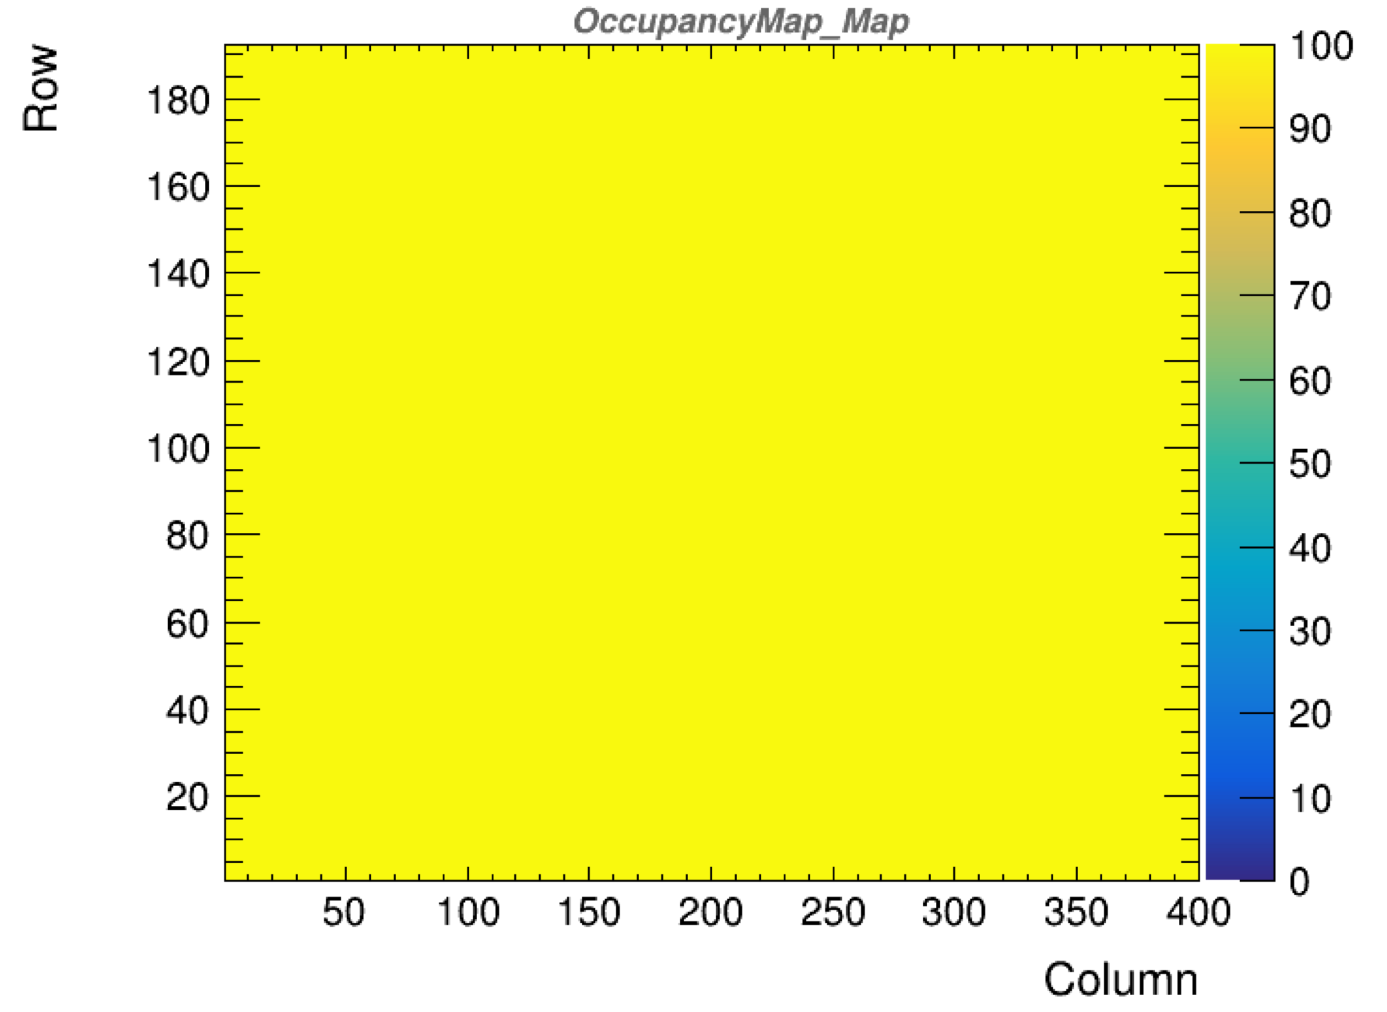
\includegraphics[width=8cm]{./dig_occ.png}
\caption[デジタル回路読み出しにおける$Occupancy$分布の例。]{デジタル回路読み出しにおける$Occupancy$分布の例。図はRD53Aを用いたデジタル回路読み出しの結果であり、横軸、縦軸はそれぞれピクセルの列(400)、行(192)に対応する。$z$軸は各ピクセルにおける$Occupancy$の値を示している。正常なピクセルは100付近になることが期待され、図では全てのピクセルで100であると分かる。}
\label{dig_occ}
\end{figure}

この試験の結果として出力されるファイルを表\ref{digital_result_files}に示す。

\begin{table}[tbp]
\begin{center}
\caption[デジタル回路読み出しにおける結果ファイル一覧]{デジタル回路読み出しにおける結果ファイル一覧。}
\label{digital_result_files}
  \small
  \begin{tabular}{|lll|} \hline
    ファイル名 & データ & ファイルサイズ \\ \hline
    OccupancyMap & 各ピクセルの$Occupancy$を記す.                           & 1.5~MB \\
    Enmask       & $Occupancy=100$のピクセルを1、それ以外を0とした値を持つ. & 1.3~MB \\ 
    L1Dist       & 信号取得タイミングの分布を持つ. & 0.53~kB \\\hline 
  \end{tabular}
\end{center}
\end{table}

\subsubsection{アナログ回路読み出し}
各ピクセルのアナログ回路部に試験用電荷を入射し、信号を取得する。
デジタル回路読み出しと同様、$Occupancy$(式\ref{occupancy})は、入射電荷数$n_i$と取得信号数$n_0$で定義され、$Occupancy$は100であることが望ましい。
試験結果として出力されるファイルはデジタル回路読み出しと同じ形式である。

\subsubsection{Threshold測定}
各ピクセルのアナログ回路部に試験用電荷を入射し、入射電荷数$n_i$と取得信号数$n_0$より$Occupancy$を測定する。
これを入射電荷量を増加させて繰り返し行う。
あるピクセルにおけるこの処理結果の例を図\ref{threshold_scurve}に示す。
\begin{figure}[bpt]\centering
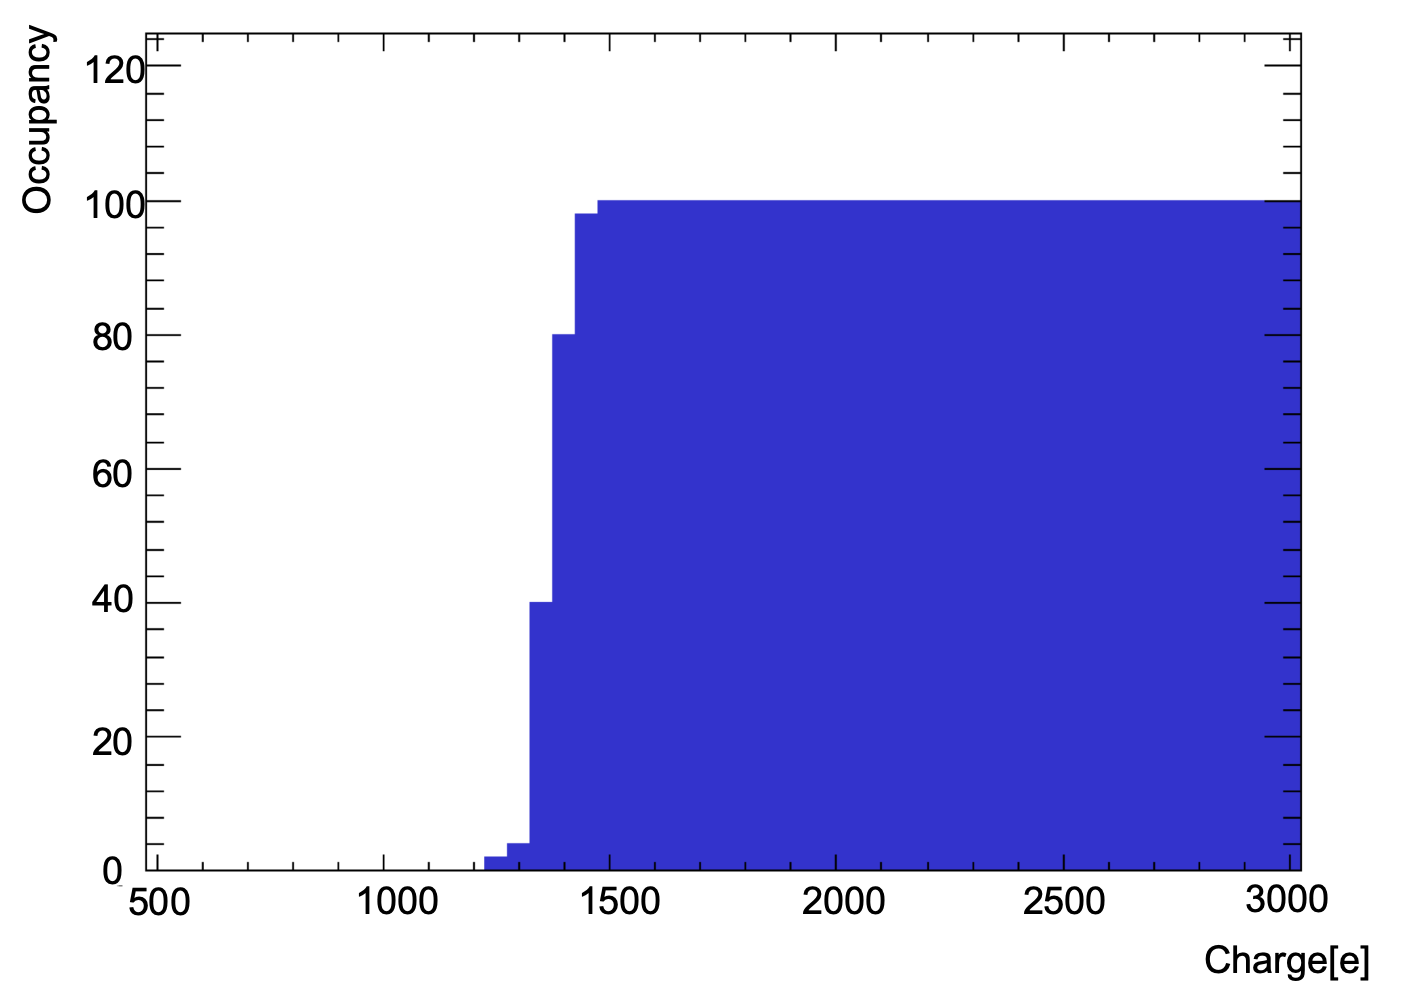
\includegraphics[width=8cm]{./threshold_scurve.png}
\caption[入射電荷量と$Occupancy$の関係]{入射電荷量と$Occupancy$の関係。横軸はピクセルに対する入射電荷量[$e$]、縦軸は$Occupancy$を示す。入射電荷量の単位$e$は、電荷量Cを素電荷$e=1.6\times 10^{-19}$[q]で割ったものである。Threshold測定の際にはこのように入射電荷量を増加させながら$Occupancy$の値を測定する。測定結果を後述する式(\ref{scurve_function})でフィットし、 Thresholdとノイズの値を得る。}
\label{threshold_scurve}
\end{figure}

この分布を以下の式でフィッティングする。フィッテングの形に由来し、これを「Sカーブフィッティング」と呼ぶ。
\bbb
\label{scurve_function}
f(x) &=& 0.5 \times \left[ 2-{\rm erfc}\left( \left\{ \frac{x-Q}{\sigma \times \sqrt{2}}  \right\} \right) \right] \times p\\
{\rm erfc}(x) &=& 1 - {\rm erf}(x)
%g(x) = \frac{2}{\sqrt{\pi}} \int_x^\infty {\rm exp}(-t^2) {\rm d}t
\eee
ここで${\rm erf}(x)$はガウスの誤差関数である\cite{3-5}。

得られた$Q$、$\sigma$がそれぞれピクセルのThreshold値、ノイズに相当する。
あるFEチップにおけるThreshold値、ノイズの分布の例を図\ref{threshold_mean_sigma}に示す。
この分布をガウス関数でフィットすることで、全ピクセルに対するThreshold、ノイズの平均値と幅が得られる。

\begin{figure}[bpt]\centering
  \begin{minipage}{0.45\hsize}
    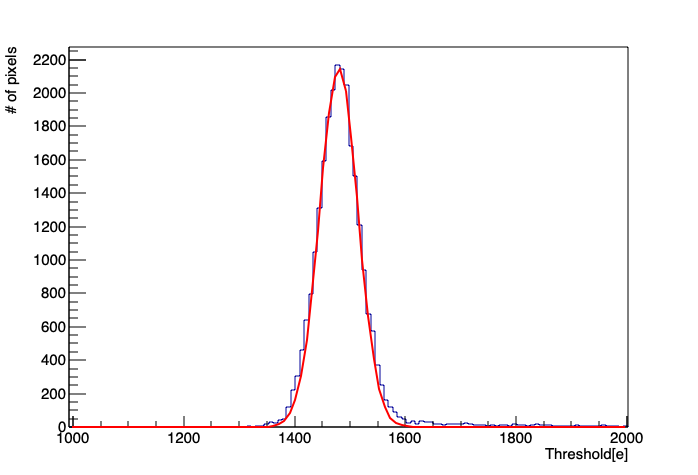
\includegraphics[width=7cm]{./data/analysis_result/Threshold_mean_dist.png}
  \end{minipage}
  \begin{minipage}{0.45\hsize}
    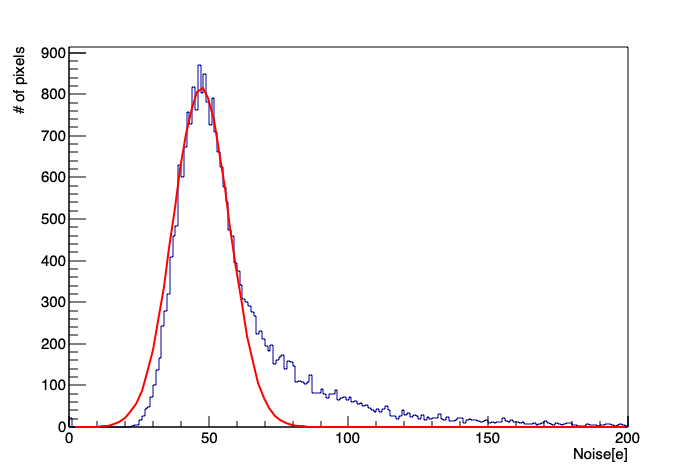
\includegraphics[width=7cm]{./data/analysis_result/Threshold_noise_dist.png}
  \end{minipage}
  \caption[Threshold値とノイズの分布。]{Threshold値とノイズの分布。図はあるFEチップ上のピクセルにおけるThreshold値(左図)とノイズ(右図)の分布を示している。また赤線はガウス関数によるフィット関数を示しており、これにより平均値と幅を取得する。}
  \label{threshold_mean_sigma}
\end{figure}

この試験において、出力される結果ファイルを表\ref{threshold_result_files}に示す。

\begin{table}[tbp]
\begin{center}
\caption[Threshold測定における結果ファイル一覧]{Threshold測定における結果ファイル一覧。}
\label{threshold_result_files}
  \small
  \begin{tabular}{|lll|} \hline
    ファイル名 & データ & ファイルサイズ \\ \hline
    ThresholdMap   & 各ピクセルのThreshold値を記す.                                                         & 2.2~MB \\
    ThresholdDist  & Thresholdの分布を記す.                                                                 & 4.6~kB \\ 
    NoiseMap       & 各ピクセルのノイズを記す.                                                              & 2.2~MB \\ 
    NoiseDist      & ノイズの分布を記す.                                                                    & 2.3~kB \\ 
    Chi2Map        & 各ピクセルのSカーブフィッティングにおける$\chi^2$の値を記す.                           & 2.3~MB \\ 
    Chi2Dist       & $\chi^2$の分布を記す.                                                                  & 1.1~kB \\ 
    StatusMap      & 各ピクセルのフィットの良さを0から5の6段階で記す.                                       & 1.3~MB \\ 
    StatusDist     & フィットの良さの分布を記す.                                                            & 0.49~kB \\ 
    TimePerFitDist & Sカーブフィットに要した時間を記す.                                                     & 3.1~kB \\ 
    Scurve         & あるピクセルの入射電荷量と$Occupancy$の関係を記す.                                     & 1.0~kB \\ 
                   & 複数のピクセルについて出力する.                                                        &        \\ 
    sCurve         & 全てのピクセルのScurveを重ね合わせた値を記す.                                          & 1.3~MB \\ \hline 
  \end{tabular}
\end{center}
\end{table}

\subsubsection{ToT測定}
各ピクセルのアナログ回路部に試験用電荷を入射し、ToTを測定する。
この操作を複数回(デフォルトでは100回)行い、平均値と幅を求める。
出力される結果ファイルを表\ref{tot_result_files}に示す。

\begin{table}[tbp]
\begin{center}
\caption[ToT測定における結果ファイル一覧]{ToT測定における結果ファイル一覧。}
\label{tot_result_files}
  \small
  \begin{tabular}{|lll|} \hline
    ファイル名 & データ & ファイルサイズ \\ \hline
    MeanToTMap   & 各ピクセルのToTの平均値を記す.   & 1.9~MB \\ 
    MeanToTDist  & ToT平均値の分布を記す.           & 0.59~kB \\ 
    SigmaToTMap  & 各ピクセルのToTの標準偏差を記す. & 2.2~MB \\ 
    SigmaToTDist & ToT標準偏差の分布を記す.         & 1.8~kB \\ 
    L1Dist       & 信号取得タイミングの分布を記す.  & 0.59~kB \\ \hline 
  \end{tabular}
\end{center}
\end{table}

\subsubsection{ノイズ占有率測定}
試験用電荷を入射せずに、周波数$f[{\rm Hz}]$、時間$t$[sec]のトリガーをかけ、取得信号数$n_0$を測定する。
YARRのデフォルトでは$f=5000、t=300$である。
$Occupancy$(式\ref{occupancy})は、発行したトリガー数$n_i=f \times t$と取得信号数$n_0$で定義される。

また$NoiseOccupancy$を以下で定義する。
$NoiseOccupancy$の分布の例を図\ref{noise_occ}に示す。
\bbb
NoiseOccupancy = \frac{n_0}{t} \times (25 \times 10^{-9})
\eee
$25 \times 10^{-9}[{\rm sec}]=25[{\rm nsec}]$は1~b.c.である。

あるピクセルにおいてノイズの量が大きいと$Occupancy$、$NoiseOccupancy$が値を持つ。
読み出しにおいてはノイズは小さいことが望まれ、これらの値は0に近いと正常なピクセルであると言える。

\begin{figure}[bpt]\centering
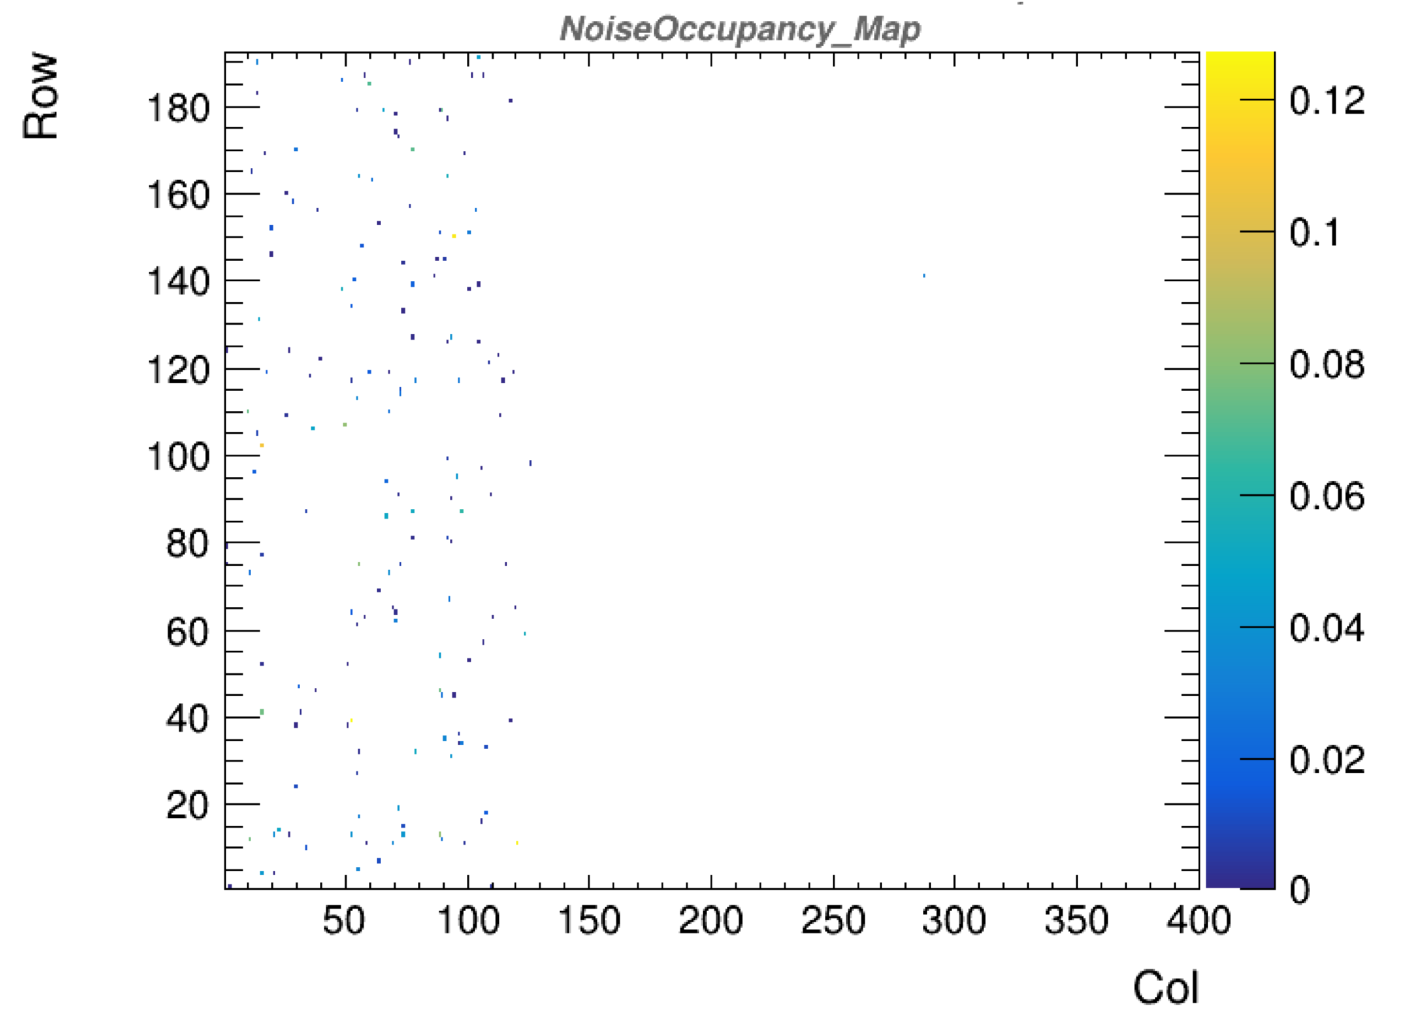
\includegraphics[width=8cm]{./noise_occ.png}
\caption[ノイズ占有率測定における$NoiseOccupancy$分布の例。]{ノイズ占有率測定における$NoiseOccupancy$分布の例。図はRD53Aを用いたデジタル回路読み出しの結果であり、横軸、縦軸はそれぞれピクセルの列(400)、行(192)に対応する。$z$軸は各ピクセルにおける$NoiseOccupancy$の値を示している。正常なピクセルでは限りなく0に近い値になることが期待され、図ではほとんどのピクセルが0となっているが、列番号が0から120付近の領域で値を大きく持つピクセルが存在する。}
\label{noise_occ}
\end{figure}

出力される結果ファイルを表\ref{noise_result_files}に示す。

\begin{table}[tbp]
\begin{center}
\caption[ノイズ占有率測定における結果ファイル一覧]{ノイズ占有率測定における結果ファイル一覧。}
\label{noise_result_files}
  \small
  \begin{tabular}{|lll|} \hline
    ファイル名 & データ & ファイルサイズ \\ \hline
    OccupancyMap      & 各ピクセルの$Occupancy$を記す. & 1.3~MB \\ 
    NoiseOccupancyMap & 各ピクセルの$NoiseOccupancy$を記す. & 1.3~MB \\ 
    NoiseMask         & $NoiseOccupancy < 10^{-6}$のピクセルを1、それ以外を0とした値を記す. & 1.3~MB \\ \hline 
  \end{tabular}
\end{center}
\end{table}

\clearpage
\subsubsection{Threshold調整とピクセル解析}\label{sec:pixel_analysis}
今後この論文では、この試験を読み出し試験と呼ぶ。
以下の流れで読み出しを行う。
\begin{itemize}
  \item デジタル回路読み出し.
  \item アナログ回路読み出し.
  \item Threshold測定.
  \item Thresholdグローバルレジスタ調整.
  \item Thresholdピクセルレジスタ調整.
  \item ToTグローバルレジスタ調整.
  \item Thresholdグローバルレジスタ再調整、精密調整.
  \item Threshold測定.
  \item ノイズ占有率測定.
  \item スタックピクセル測定.
  \item クロストーク測定.
\end{itemize}
この試験の中では読み出し回路の性能確認に加えて、各ピクセルが持つThreshold、ToTをある共通値に近づける調整を行う。

測定後、試験結果の解析を行い、モジュール上の各ピクセルが正常かどうかを判断する。
設定されている評価基準を表\ref{pixel_analysis_criteria}に示す。不良ピクセルには評価基準に応じた評価名が付けられる。

\begin{table}[tbp]
\begin{center}
\caption[ピクセル解析の評価基準一覧]{ピクセル解析の評価基準一覧\cite{3-1}。読み出し試験において各ピクセルが正常に機能しているかを判断するためにピクセル解析を行う必要があり、それの判断基準が表のように定義されている。この基準一覧は不良評価であり、全ての基準に当てはまらないピクセルが良好と判断される。不良ピクセルの数や分布は、モジュールの品質を決定する1つの要素となり、ITkに搭載するモジュールの選択や配置の決定に用いられる。}
\label{pixel_analysis_criteria}
  \small
  \begin{tabular}{|lll|} \hline
    評価名 & 読み出し項目 & 評価基準 \\ \hline
    Digital Dead      & Digital scan           & $Occupancy < 1$ \\ \hline
    Digital Bad       & Digital scan           & $Occupancy < 98 \: or \: Occupancy > 102$ \\\hline 
    Merged Bump       & Analog scan            & $Occupancy < 98 \: or \: Occupancy > 102$  \\ 
                      & Crosstalk scan         & High Crosstalk\\ \hline
    Analog Dead       & Analog scan            & $Occupancy < 1$ \\ \hline
    Analog Bad        & Analog scan            & $Occupancy < 98 \: or \: Occupancy > 102$ \\ \hline
    Tuning Failed     & Threshold scan         & Sカーブフィット失敗(YARRでは$\chi^2=0$となる) \\ \hline
    Tuning Bad        & Thresheld scan         & $|{\rm Threshold}-{\rm Threshold}_{\rm 平均}| > 5 \times {\rm Threshold}_{\rm 幅}$ \\ 
                      & ToT scan               & ToT $ = 0 \: or \: 15 $\\ \hline
    High ENC          & Threshold scan         & $|ノイズ-ノイズ_{\rm 平均}| > 3 \times ノイズ_{\rm 幅}$\\ \hline
    Noisy             & Noise scan             & $NoiseOccupancy > 10^{-6}$\\ \hline
    Disconnected Bump & Disconnected bump scan & 現段階では未決定 \\ 
                      & Source scan            & $Occupancy$がFEチップ全体平均の$1\%$ \\ \hline
    High Crosstalk    & Crosstalk scan         & $Occupancy>0 \: with \: 25{\rm ke}$ (sync FE)\\
                      &                        & $Occupancy>0 \: with \: 40{\rm ke}$ (lin and diff FE)\\ \hline 
  \end{tabular}
\end{center}
\end{table}

\clearpage
\subsubsection{簡易読み出し試験}
品質試験項目の1つに、以下の項目を扱う簡易読み出し試験がある。
\begin{itemize}
  \item レジスタの読み書き.
  \item デジタル回路読み出し.
  \item アナログ回路読み出し.
  \item Threshold測定.
  \item ToT測定.
  \item バンプ接続確認測定.
\end{itemize}

\subsection{各組み立て工程における品質試験}

各組み立て工程と品質試験項目を図\ref{stage_test_flow}に示す。
図より、1モジュールに対して行われる品質試験は30程度存在することが分かる。

\begin{figure}[bpt]\centering
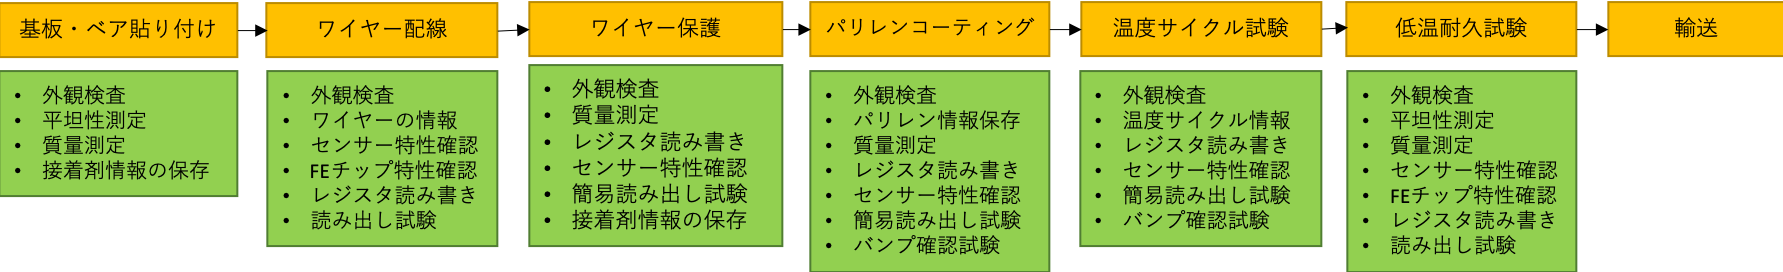
\includegraphics[width=15cm]{./stage_test_flow.png}
\caption[組み立て工程と対応する品質試験一覧]{組み立て工程と対応する品質試験一覧。節\ref{sec:assembly}で述べた各組み立て工程において、複数の品質試験を行う必要がある。図は各組み立て工程と対応する品質試験一覧を示している。試験数は30程度存在する。}
\label{stage_test_flow}
\end{figure}

\section{検出器量産におけるデータ管理}
各組み立て機関で$O(100)〜O(1,000)$のモジュールを作り、上述したように1モジュールに対して30程度の品質試験を行う。
1,000モジュール作る機関であれば3,000の試験結果が得られる。この数の品質試験結果を正確に管理することが必要となる。
特に読み出し試験については、1試験につき更に細かい項目に細分化され、項目、結果ファイルも多様である。
これらの情報は最終的に共通のデータベースに保存する必要があり、各組み立て機関で適切に管理する必要がある。

本研究では各組み立て機関におけるモジュール情報及び品質試験のデータ管理を簡易化することを目的として、データベースシステムの構築を行った。
このシステムについて\ref{chap:dbsystem}章で説明する。


\chapter{モジュール情報及び品質試験結果管理システム}\label{chap:dbsystem}
前章で述べたように、モジュール生産及び品質試験を世界中で行う。
これらの情報はデータベースシステムを用いて管理することが決定していて、現在この開発を行っている。
システムについては、ITkの全情報を保存する中央データベースと、各組み立て機関に設置し、データ管理を行うローカルデータベースである。
本章ではこれらのデータベースについて説明する。また、システム開発の中で私が開発を行った機能について詳細に説明する。

%%%%%%%%%%%%%%%%%%%%%%%%%%%%%%%%%%%%%%%%%%%%%%%%%
%%%%%%%%%%%%%%%%%%%%%%%%%%%%%%%%%%%%%%%%%%%%%%%%%
%%%%%%%%%%%%%%%%%%%%%%%%%%%%%%%%%%%%%%%%%%%%%%%%%
\section{中央データベース}
\subsection{中央データベースの概要}
\subsubsection{概要}
中央データベースは、ITkの製造に関する全ての情報の保存を目的として開発されたデータベースである。
ユニコーン大学が開発、運用を行っていて、チェコにデータベースサーバーが設けられている。
ITkは、ピクセル検出機とストリップ検出機にから構成される。
これらを生産するにあたって、シリコンセンサーやフレキシブル基板といった小さな部品から製造を行い、それらを用いたモジュールの組み立て、複数モジュールを搭載したステーブやリングの組み立てを経て検出器が完成する。
また各組み立て段階において、動作確認等を目的とした品質試験を行う。
これらの過程における全ての構成部品の情報、及び品質試験結果を中央データベースに保存する。

\subsubsection{意義}
中央データベースを扱う一番の目的は、ITkに用いるモジュールの選別とその配置の決定に用いることである。
品質試験結果を解析、品質のいいモジュールを10,000台の中から選別、ITkに搭載する。
また、モジュールの配置も品質を考慮して決定する。
例として以下の2つをあげる。
\begin{itemize}
  \item $|\eta|$が小さい領域には、不良ピクセルが少なく品質の良いモジュールを搭載する.
  \item 不良ピクセルの領域が固まらないようにする.
\end{itemize}

次に中央データベースに保存された情報は、検出器運転時の参考値として扱われる。
モジュールを例にだすと、品質試験で読み出し試験を行った際の最適な設定値を中央データベースに保存するため、実際の運転時に参照することができる。
また運転前の状態における検出器の性能、運転前後での性能比較を行うことができる。

\clearpage
%%%%%%%%%%%%%%%%%%%%%%%%%%%%%%%%%%%%%%%%%%%%%%%%%
%%%%%%%%%%%%%%%%%%%%%%%%%%%%%%%%%%%%%%%%%%%%%%%%%
%%%%%%%%%%%%%%%%%%%%%%%%%%%%%%%%%%%%%%%%%%%%%%%%%
\section{ローカルデータベース}
\subsection{ローカルデータベースの意義と概要}
中央データベースでは、前述したようにモジュールの情報のみならずITkに関わるすべての情報を管理する。データベースの機能としては汎用的に使えるようなものになっている。
モジュールの組み立て及びその品質試験に関しては3章で述べたように工程が複数に渡り、行う品質試験の数も多い。
1つの生産現場で多いところでは数千個のモジュールを作ることになるため、
データ管理が簡単にかつ円滑に進むようになっているのが好ましい。
このような理由から、生産現場での生産性、利便性に特化し、円滑な生産をサポートすることを目的としたデータベースシステム(ローカルデータベース)を開発している。
システムの概要図を図\ref{localdb_overview}に示す。オープンソースのサービスであるMongoDB\cite{4-1}と、
PythonのウェブフレームワークであるFlask\cite{4-3}を使用し、開発を行なっているローカルデータベース用ウェブアプリケーションを併用することで、データ管理や中央データベースとの同期を行うシステムとなっている。

ローカルデータベースシステムには以下のような利点を持ち得る。
これらの利点を持つシステムの開発、実装を行うことが開発課題となっている。

\begin{itemize}
  \item ローカルにデータベースサーバーを立てるためアクセス速度が早く、円滑にデータ管理を行うことができる。
  \item モジュールの組み立て工程を管理し、生産者の適切な処理を助ける。
  \item モジュールに特化したデータ管理、解析を行うことで異常をいち早く検知できる。
  \item 試験者の情報や試験時間など、品質試験結果以外の必要な情報を正確に管理できる。
\end{itemize}

\begin{figure}[bpt]\centering
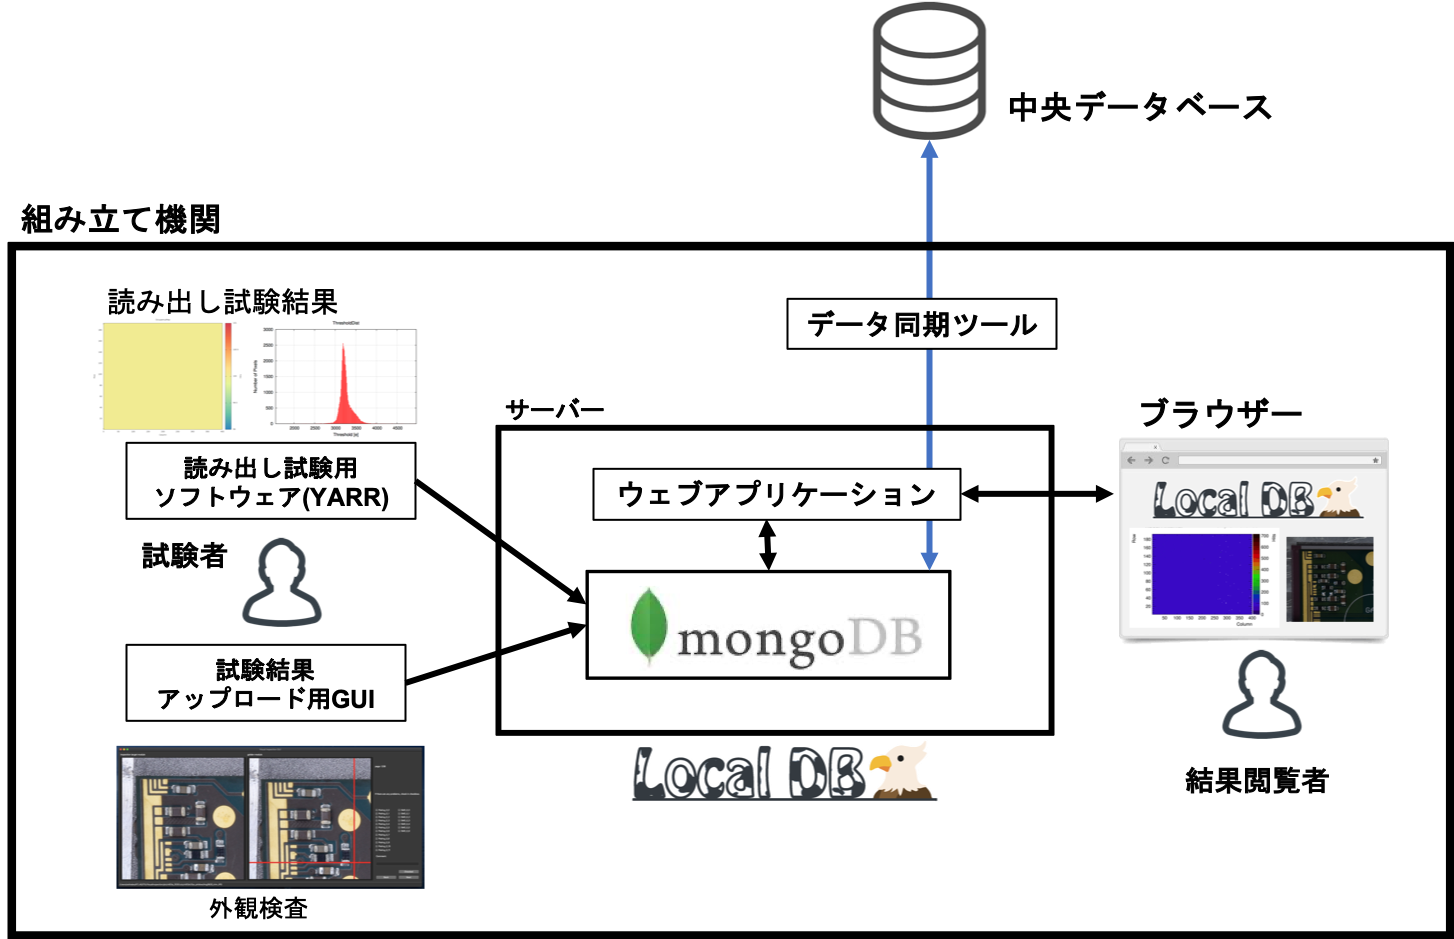
\includegraphics[width=12cm]{./localdb_overview.png}
\caption[ローカルデータベースシステムの概要]{ローカルデータベースシステムの概要。各組み立て機関でMongoDBとローカルデータベース用ウェブアプリケーションの立ち上げを行い、独自にデータ管理をするシステムとなっている。品質試験者は図のようにいくつかのソフトウェアを用いて試験結果をMongoDBに保存する。保存された結果はウェブアプリケーションによって閲覧することができる。また結果は中央データベースに集める必要があるため、同期ツールを用いて試験結果の共有を行う。}
\label{localdb_overview}
\end{figure}

\subsection{先行研究と開発課題}
先行研究で開発された領域と、本研究で取り組んだ開発課題を以下に示す。

\subsubsection{先行研究}
先行研究\cite{4-6}においてデータベースシステムの設計と開発がなされ、図\ref{localdb_overview}におけるいくつかの項目が開発された。
以下に実装項目を記す。
\begin{enumerate}
  \item 読み出し試験結果保存のためのMongoDB内部構造の設計.
  \item 1の構造を用いてYARRからMongoDBへの読み出し試験結果アップロード機能.
  \item 試験結果のソート及び閲覧が可能な、Flaskを用いたウェブアプリケーション. 
\end{enumerate}

モジュールの生産、品質試験に向けたデータ管理、そしてローカルデータベースが上述した利点を持つことを達成するには以下のような開発課題が残されていた。
\begin{itemize}
  \item 中央データベースの内部構造の実装.
  \item 中央データベースとローカルデータベース間の同期ツールの開発.
  \item ローカルデータベースにおける品質試験に特化したデータ管理と機能提供.
  \item 量産時におけるデータベース操作の流れの確立.
\end{itemize}

これらの開発課題に対して、本研究で取り組んだ項目を以下に挙げる。
なお先行研究で開発したデータ構造やアプリケーションといった項目は既に複数の機関で試験運用されていたため、本研究ではその構造やソフトウェアを大きく変更せずに、拡張する形で開発を行なった。

\subsubsection{中央データベースの内部構造の実装}
モジュール及び品質試験の結果を中央データベースに登録するために、モジュールの種類や品質試験項目など中央データベースにおける内部構造の実装する必要がある。本研究ではこういった量産時において必要となるデータ構造の実装を行なった。

\subsubsection{中央データベースとローカルデータベース間の同期ツールの開発}
ローカルデータベースを各組み立て機関に設置し、データ管理を行う。
中央データベースに必要な情報が全て保存されるためにはデータベース間の同期が必要である。
これを達成するために中央データベースとローカルデータベースの同期を行うツール開発を行なった。

\subsubsection{ローカルデータベースにおける品質試験に特化したデータ管理と機能提供}
ローカルデータベースにおける利点の1つである「品質試験に特化したデータ管理と機能提供」を達成するために以下の機能を実装した。
\begin{itemize}
  \item 品質試験者及びシステムユーザ管理機能及びコメント付加等の各種機能.
  \item 品質試験結果の登録と組み立て工程の自動更新.
  \item 読み出し試験におけるピクセル解析ツールの開発.
  \item 読み出し試験結果の検索機能.
\end{itemize}

\subsubsection{量産時におけるデータベース操作の流れの確立}
先行研究では品質試験の際に、登録、同期といったデータベース操作の流れが確立されていなかった。
本研究では上述した機能開発と併せて、品質試験におけるデータ管理の流れを確立した。

%%%%%%%%%%%%%%%%%%%%%%%%%%%%%%%%%%%%%%%%%%%%%%%%%
%%%%%%%%%%%%%%%%%%%%%%%%%%%%%%%%%%%%%%%%%%%%%%%%%
%%%%%%%%%%%%%%%%%%%%%%%%%%%%%%%%%%%%%%%%%%%%%%%%%
\subsection{MongoDBと内部構造\cite{4-2}}
MongoDBとはNoSQLに分類されるデータベースである。
MongoDBの構造について簡単に表したものを図\ref{mongodb_schema}に示す。
一般的なSQLDBのようにテーブル形式ではなく、JSON形式で情報を格納する。
情報を保持している一枚のJSONインスタンスを「\textbf{ドキュメント}」と呼び、「\textbf{コレクション}」と呼ばれる枠に複数のドキュメントが格納されている。
各ドキュメントは「\textbf{ID}」と呼ばれるハッシュ値を持っていて、異なるコレクションにおけるドキュメント間の紐付けはこのIDを用いて行う。

\begin{figure}[bpt]\centering
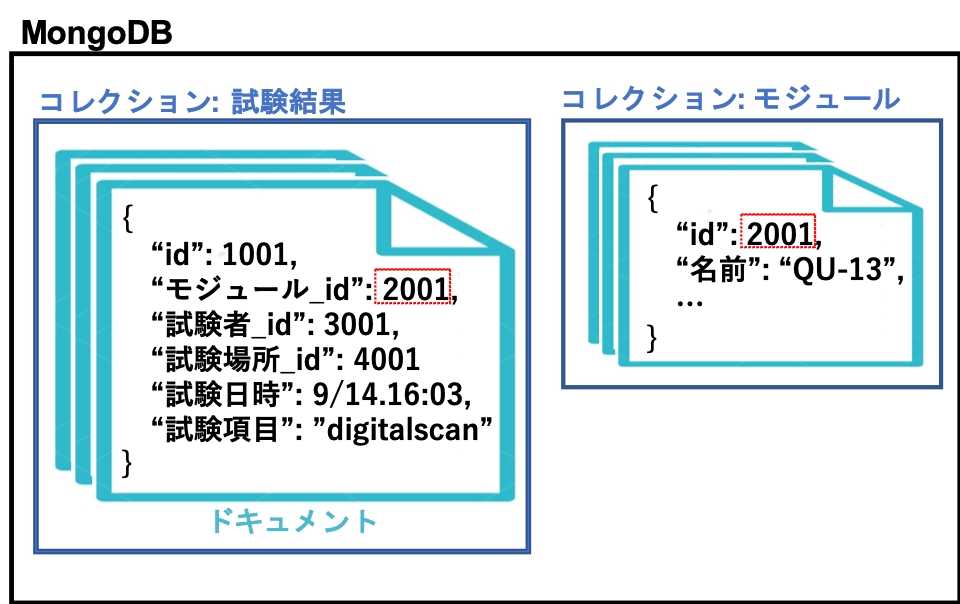
\includegraphics[width=12cm]{./mongodb_schema.png}
\caption[MongoDBの構造の例\cite{4-2}]{MongoDBの構造の例\cite{4-2}。図のようにMongoDBではJSON形式でデータを格納する。1枚のJSONインスタンスをドキュメントと呼び、複数のドキュメントが格納されている枠組みをコレクションと呼ぶ。ドキュメントの構造及びコレクション間の関係等を決めることでデータベースの構造を定義する。ドキュメント間の紐付けは、各ドキュメント内部にIDを持つことで可能となる。図の例では試験結果のドキュメントが$\{$``モジュール$\_$id":2001$\}$の情報を持っており、これがモジュールに保存されているドキュメントの1枚目のIDに対応する。}
\label{mongodb_schema}
\end{figure}


ローカルデータベースシステムにおいて、MongoDBを使用する主な利点を以下に示す。

\begin{itemize}
  \item 各コレクションに格納するドキュメントの構造が動的であるため、開発を柔軟に行うことができる。
  \item JSON形式でデータを保持するため情報取得の際の整形処理をが容易であり、ウェブアプリケーションとの親和性が高い。
  \item データのキャッシュをメモリ上に置き処理を実行するため、高速な読み書きが可能。
\end{itemize}

モジュール及び品質試験に用いる主なコレクションを表\ref{localdb_structure}に示す。
また先行研究で設計された読み出し試験に関する内部構造の詳細と関係性を図\ref{localdb_structure_detail}に示す。

%%%%%%%%%%%%%%%%%%%%%%%%%%%%%%%%%%%%%%%%%%%%%%%%%
%%%%%%%%%%%%%%%%%%%%%%%%%%%%%%%%%%%%%%%%%%%%%%%%%
%%%%%%%%%%%%%%%%%%%%%%%%%%%%%%%%%%%%%%%%%%%%%%%%%
\begin{table}[btp]
\begin{center}
\caption[品質試験に用いる主なコレクション]{品質試験に用いる主なコレクション。ローカルデータベースシステムにおいて、MongoDB内に2つのデータベースを設置し、使用する。}
\label{localdb_structure}
  \small
  \begin{tabular}{|lll|} \hline
    データベース名 & コレクション名 & 情報 \\ \hline
    localdb      & component & モジュール情報、FEチップ情報 \\ 
                 & childParentRelation & FEチップとモジュールの関係性 \\ 
                 & QC.module.status & 各モジュールに対する組み立て工程及び選択された試験結果 \\ 
                 & QC.result & 品質試験結果 \\ 
                 & testRun & 読み出し試験結果 \\ 
                 & user & 読み出し試験実施者 \\
                 & institute & 読み出し試験実施場所 \\
                 & componentTestRun & componentとtestRunの関係性 \\
                 & comments & コメント情報 \\ \hline
    localdbtools & QC.status & 組み立て工程及び試験項目\\
                 & viewer.user & 登録ユーザの情報 \\
                 & viewer.query & 読み出し結果キーワード、検索機能実行時に使用 \\ 
                 & viewer.tag.docs & モジュールや試験結果に付けるタグの情報 \\ \hline
  \end{tabular}
\end{center}
\end{table}

\begin{figure}[bpt]\centering
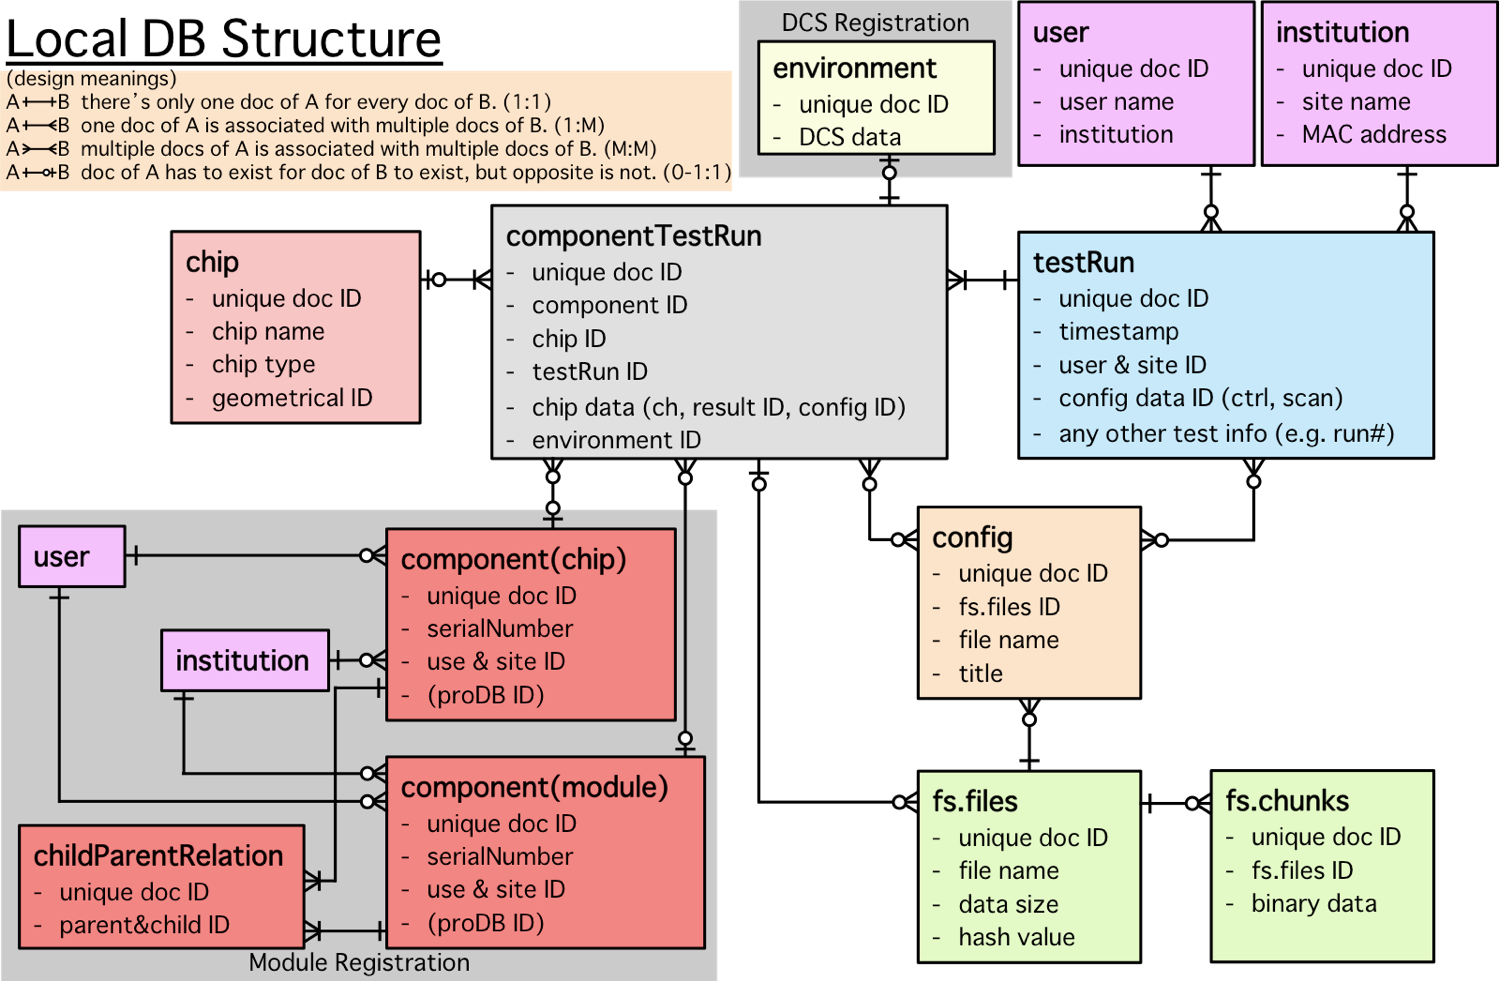
\includegraphics[width=12cm]{./localdb_structure_detail.png}
\caption[先行研究により設計された読み出し試験結果のMongoDB内部構造]{先行研究により設計された読み出し試験結果のMongoDB内部構造\cite{4-6}。それぞれの四角はコレクション、直線はIDによるドキュメント間のリンクを示している。直線が十字になっている場合はドキュメント間が一対一対応であることを示し、分岐しているものは複数のドキュメントと対応していることを示す。また直線状の白丸は対応するドキュメントが存在しない場合があることを示している。}
\label{localdb_structure_detail}
\end{figure}

\clearpage
%%%%%%%%%%%%%%%%%%%%%%%%%%%%%%%%%%%%%%%%%%%%%%%%%
%%%%%%%%%%%%%%%%%%%%%%%%%%%%%%%%%%%%%%%%%%%%%%%%%
%%%%%%%%%%%%%%%%%%%%%%%%%%%%%%%%%%%%%%%%%%%%%%%%%
\subsection{ウェブアプリケーション} \label{sec:web_app}

各組み立て機関において、試験者が品質試験結果を閲覧、管理するツールとして、ウェブアプリケーションを提供している。
アプリケーション開発には、PythonのウェブフレームワークであるFlaskを使用している。
またアプリーケーションにおいてMongoDBとの通信に用いるAPIとして、PythonライブラリであるPyMongo\cite{4-4}を用いている。
ローカルデータベースとアプリケーション間の処理に特化したイメージを図\ref{webapp_process}に示す。
このようにアプリケーションはデータベースとブラウザー、データベース間のインターフェースとなっている。

試験結果を迅速に分かりやすく見るシステムを作り、円滑な生産の補助や異常結果の早期発見を目的としている。
またデータベースの情報管理のみならず、同期ツールや、後述する試験結果解析ツールなどの外部スクリプトの実行、結果取得等、生産時における多くのデータベース操作はこのアプリケーションを用いて行う。

ウェブアプリケーションでは、現在以下の機能を使用することができる。ある品質試験の結果ページを図\ref{viewer_result}に示す。
\begin{itemize}
  \item 登録モジュール情報及び品質試験結果の閲覧、解析
  \item ローカルデータベースにおけるユーザ管理機能
  \item データベース同期実行機能
\end{itemize}

\begin{figure}[bpt]\centering
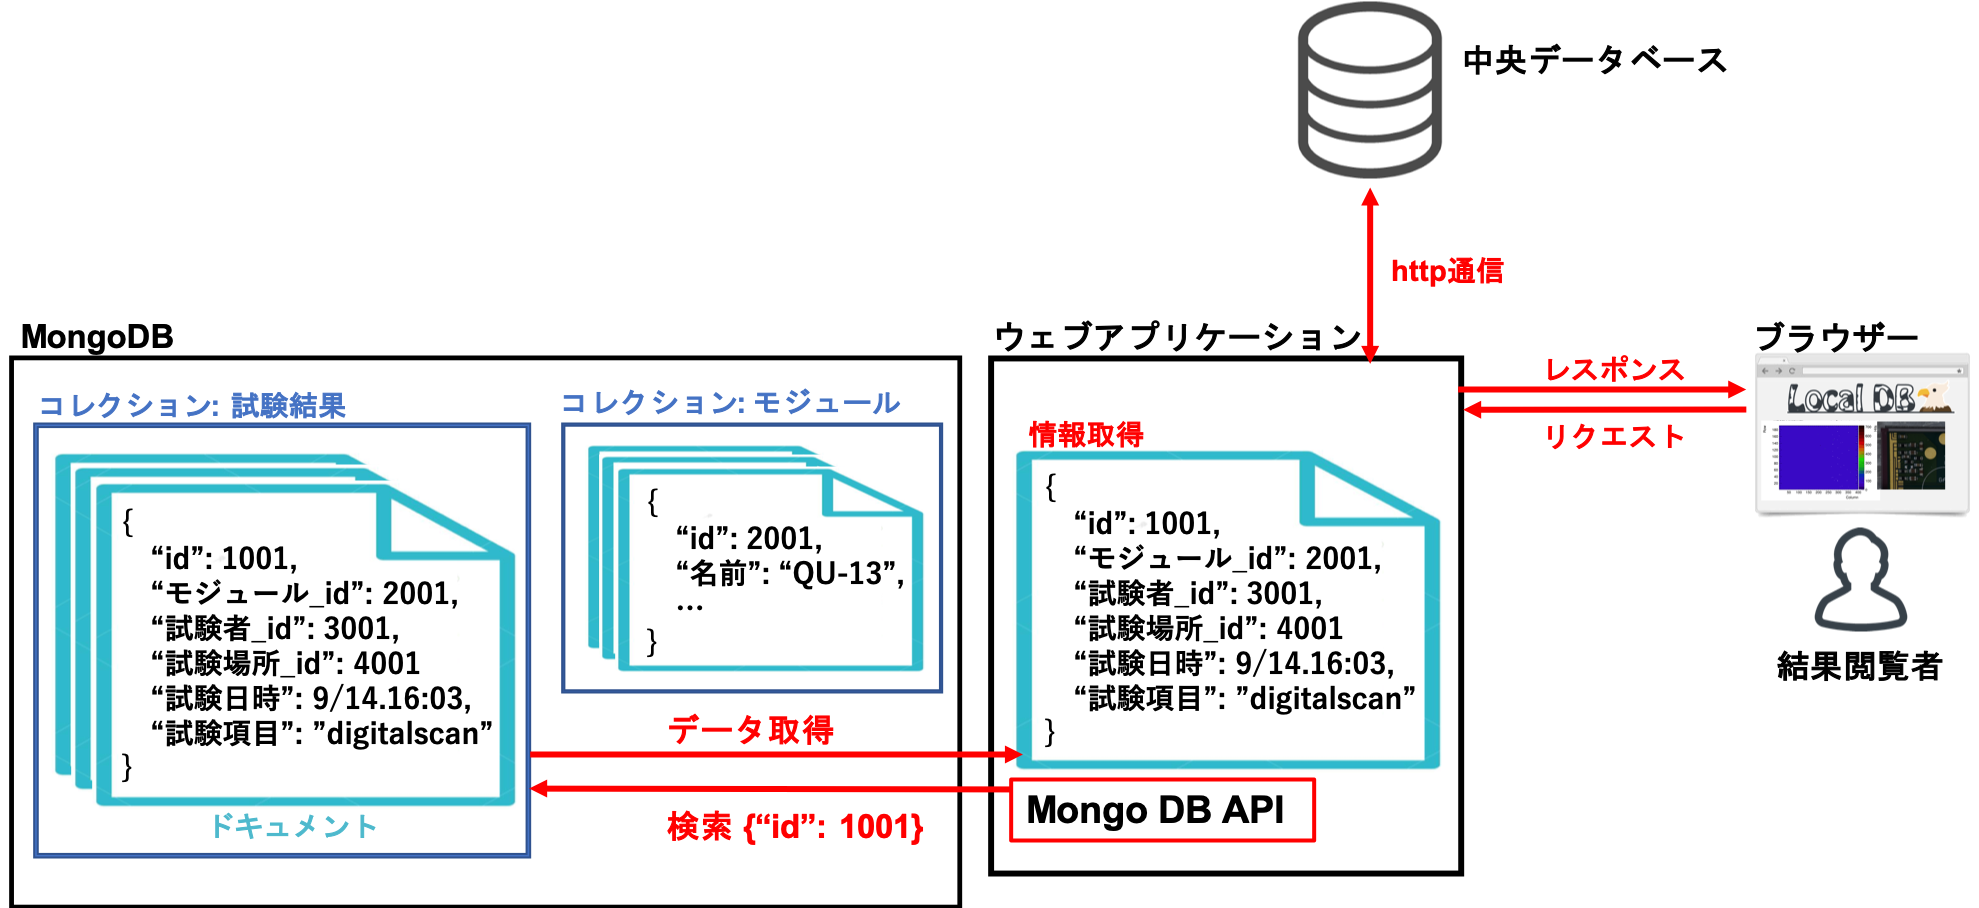
\includegraphics[width=16cm]{./webapp_process.png}
\caption[ウェブアプリケーション処理のイメージ]{ウェブアプリケーション処理のイメージ。ウェブアプリケーションではMongoDB通信API(PyMongo)を用いて、データベースのコレクションに検索をかけることで情報を取得する。取得した情報は整形されたのちブラウザに送信、中央データベースとの同期等の処理に用いられる。}
\label{webapp_process}
\end{figure}

\begin{figure}[bpt]\centering
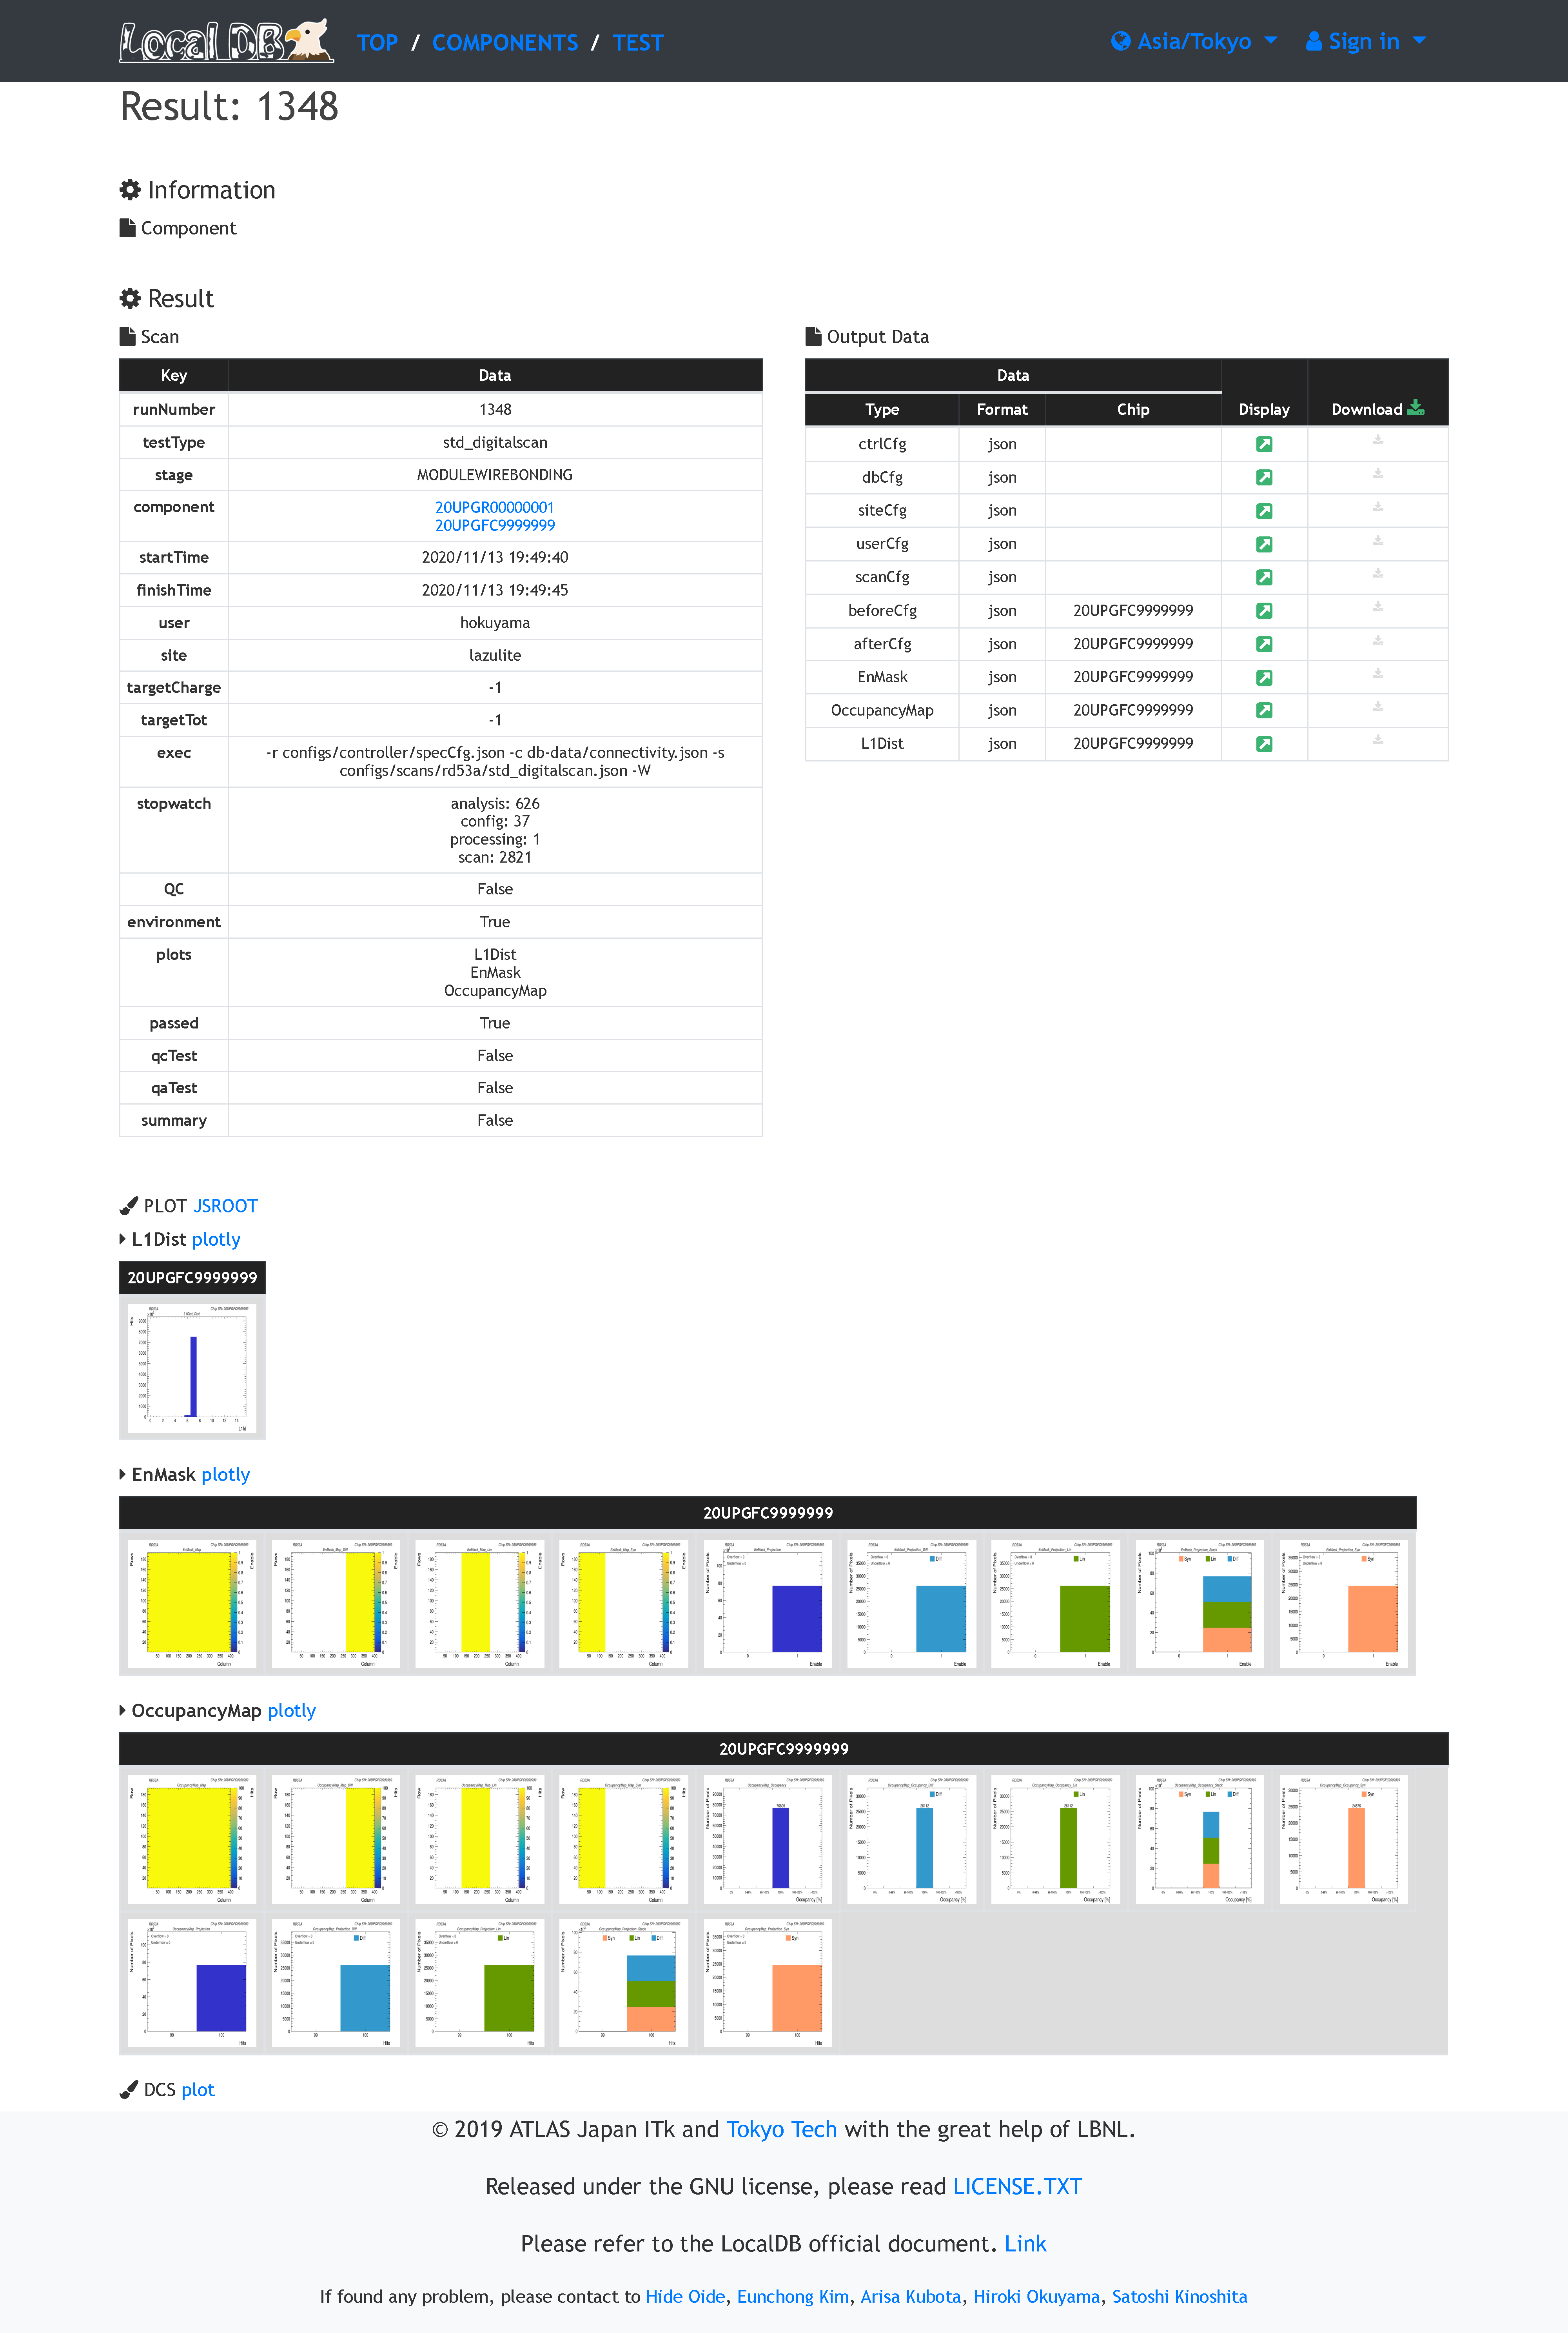
\includegraphics[width=15cm]{./demo_view_scan_result.pdf}
\caption[品質試験結果ページの例]{品質試験結果ページの例。図は品質試験項目であるデジタル回路読み出しの結果を表している。図の上部に試験情報や設定値、下部に結果のグラフが表示されているのを確認できる。}
\label{viewer_result}
\end{figure}


\clearpage
%%%%%%%%%%%%%%%%%%%%%%%%%%%%%%%%%%%%%%%%%%%%%%%%%%%
%%%%%%%%%%%%%%%%%%%%%%%%%%%%%%%%%%%%%%%%%%%%%%%%%%%
%%%%%%%%%%%%%%%%%%%%%%%%%%%%%%%%%%%%%%%%%%%%%%%%%%%
\section{本研究における開発項目の詳細}
以下は本研究で開発した項目である。

%%%%%%%%%%%%%%%%%%%%%%%%%%%%%%%%%%%%%%%%%%%%%%%%%%%
%%%%%%%%%%%%%%%%%%%%%%%%%%%%%%%%%%%%%%%%%%%%%%%%%%%
%%%%%%%%%%%%%%%%%%%%%%%%%%%%%%%%%%%%%%%%%%%%%%%%%%%
\subsection{中央データベースの内部データ構造の実装}

モジュール及びその品質試験に関する情報を中央データベースに情報を保存するために、情報構造の定義、実装を行う必要がある。
以下の項目について、中央データベースが提供しているAPIを用いて内部データ構造の定義を行った。
\begin{enumerate}
  \item モジュールの種類とその構成部品(図\ref{pd_module_structure}).
  \item モジュール組み立て工程と付随する品質試験(表\ref{pd_stage_structure}).
\end{enumerate}

また項目1に関して、Quadモジュールに関する例を図\ref{example_module_structure}に示す。

%\begin{table}[b]
%\begin{center}
%\caption[中央データベースにおけるモジュールの種類と構造一覧]{中央データベースにおけるモジュールの種類と構造一覧。中央データベースにモジュールを登録するときの情報として、モジュールの種類、構成部品を表のように実装した。Triplet、Quadというように、モジュールの種類ごとに登録できるシステムとなっており、PCB(フレキシブル基板)などの対応する構成部品の紐付けも同時に行うことができる。}
%\label{pd_module_structure}
%  \scriptsize
%  \begin{tabular}{|ll|} \hline
%    種類 & 構成する部品(数) \\ \hline
%    Triplet L0 stave module   &  Single bare module(3) \\
%                              &  Triplet stave PCB(1) \\\hline
%    Triplet L0 Ring0 module   &  Single bare module(3) \\
%                              &  Triplet R0 PCB(1) \\\hline
%    Triplet L0 Ring0.5 module &  Single bare module(3) \\
%                              &  Triplet R0.5 PCB(1) \\\hline
%    L1 quad module            &  Quad bare module(1) \\
%                              &  Quad PCB(1) \\\hline
%    Outer system quad moudle  &  Quad bare module(1) \\
%                              &  Quad PCB(1) \\\hline
%    Outer system quad moudle  &  Dual bare module(1) \\
%                              &  Dual PCB(1) \\\hline
%    Digital triplet L0 stave module   &  Digital single bare module(3) \\
%                                      &  Triplet stave PCB(1) \\\hline
%    Digital triplet L0 Ring0 module   &  Digital single bare module(3) \\
%                                      &  Triplet R0 PCB(1) \\\hline
%    Digital triplet L0 Ring0.5 module &  Digital single bare module(3) \\
%                                      &  Triplet R0.5 PCB(1) \\\hline
%    Digital quad module       &  Digital quad bare module(1) \\
%                              &  Quad PCB(1) \\\hline
%    Digital L1 quad moudle    &  Digital quad bare module(1) \\
%                              &  Quad PCB(1) \\\hline
%    Dummy triplet L0 stave module   &  Dummy single bare module(3) \\
%                                    &  Triplet stave PCB(1) \\\hline
%    Dummy triplet L0 Ring0 module   &  Dummy single bare module(3) \\
%                                    &  Triplet R0 PCB(1) \\\hline
%    Dummy triplet L0 Ring0.5 module &  Dummy single bare module(3) \\
%                                    &  Triplet R0.5 PCB(1) \\\hline
%    Dummy quad module       &  Dummy quad bare module(1) \\
%                            &  Quad PCB(1) \\\hline
%    Dummy L1 quad moudle    &  Dummyl quad bare module(1) \\
%                            &  Quad PCB(1) \\ \hline
%  \end{tabular}
%\end{center}
%\end{table}

\begin{figure}[b]\centering
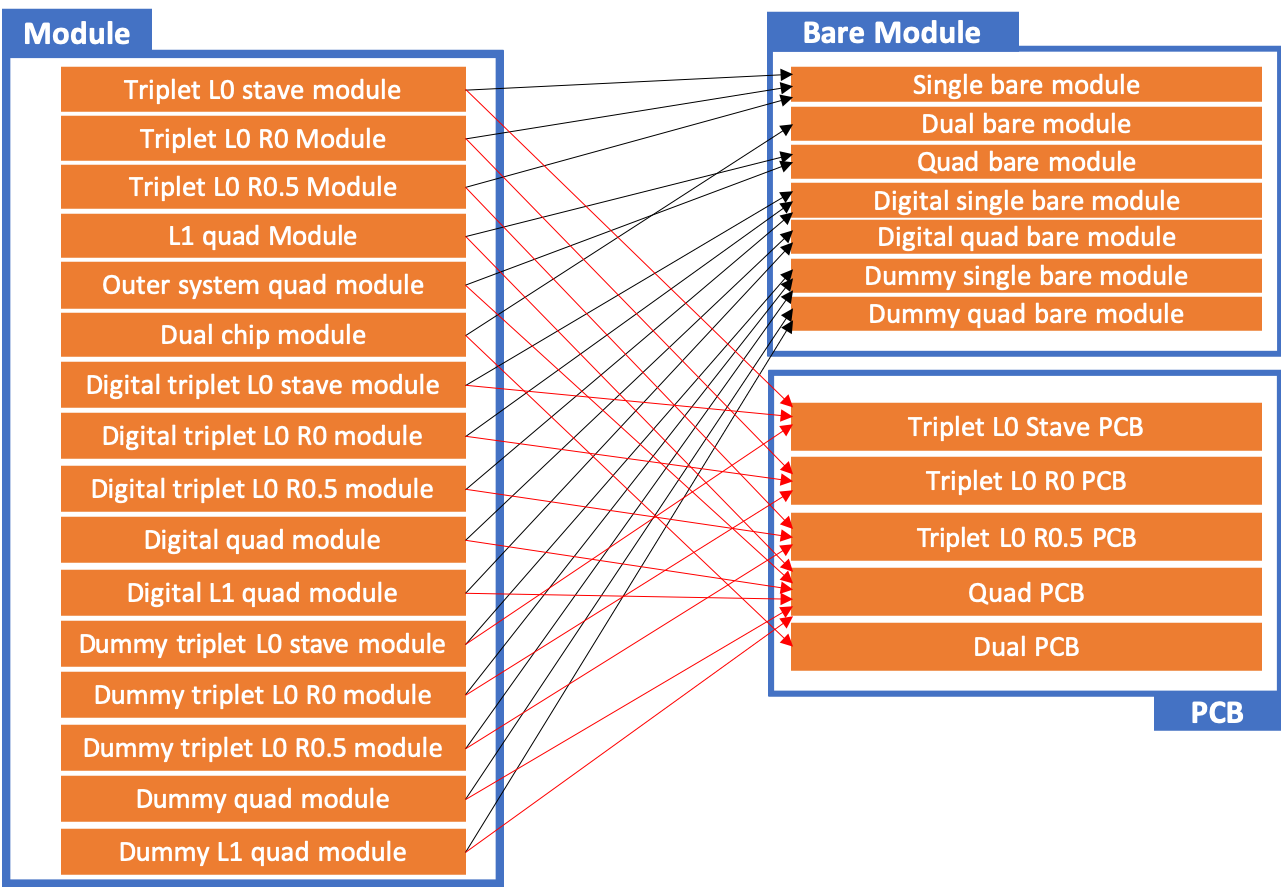
\includegraphics[width=12cm]{./pd_module_structure.png}
\caption[中央データベースにおけるモジュールの種類と構造]{中央データベースにおけるモジュールの種類と構造。中央データベースにモジュールを登録するときの情報として、モジュールの種類、構成部品を図のように実装した。図の左側に実装したモジュールの種類を示しており、Triplet、Quadというように、モジュールの種類ごとに登録できるシステムとなっている。また矢印は構成部品を指しており、各モジュールは対応するBare Module(ベアモジュール)とPCB(フレキシブル基板)を持つ。DBの中でモジュールと構成部品の紐付けも同時に行うことができる。}
\label{pd_module_structure}
\end{figure}

\begin{figure}[bpt]\centering
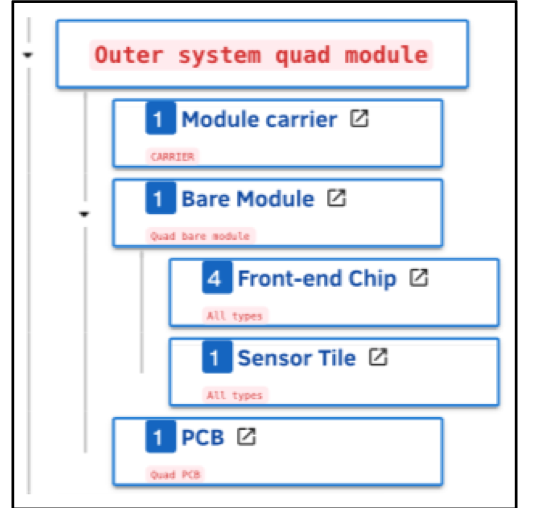
\includegraphics[width=6cm]{./example_module_structure.png}
\caption[中央データベース内におけるモジュール構造の一例(Quadモジュール)]{中央データベース内におけるモジュール構造の一例(Quadモジュール)。例としてOuter system quad moduleの中央データベース内の構造を示している。この種類では構成要素としてそれぞれ対応する種類のModule carrier、Bare Module、PCBを持つことがわかる。さらにBare ModuleはFE chipを4、Sensorを1持つことが分かり、Quadモジュールの構造が正しく実装されていることが分かる。}
\label{example_module_structure}
\end{figure}

\begin{table}[btp]
\begin{center}
\caption[中央データベースにおける組み立て工程と付随するテスト項目]{中央データベースにおける組み立て工程と付随するテスト項目。モジュールの組み立て工程及び品質試験を登録するため、表のような構造を実装した。データベース内でこの表に沿った組み立て工程の登録、更新、試験結果のアップロードができるようになった。}
\label{pd_stage_structure}
  \scriptsize
  \begin{tabular}{|ll|} \hline
    組み立て項目 & 付随する組み立て情報及び品質試験項目 \\ \hline
    1. Bare to PCB assembly & Visual Inspection \\ 
                            & Metrology \\
                            & Mass measurement \\
                            & Glue information \\\hline
    2. Wirebonding          & Visual Inspection \\ 
                            & Wirebond information \\
                            & (Wirebond pull test)\\
                            & First power up\\
                            & Sensor IV\\
                            & SLDO VI\\
                            & Chip configuration\\
                            & Pixel failure test\\\hline

    3. Wirebond Protection  & Visual Inspection \\ 
                            & Potting information \\
                            & Sensor IV \\
                            & Register test\\
                            & Readout for basic electrical \\\hline

    4. Parylene Coating     & Visual Inspection \\ 
                            & Palylene information \\
                            & Mass measurement \\
                            & Sensor IV \\
                            & Register test\\
                            & Readout for basic electrical \\
                            & Bump bond quality \\\hline

    5. Thermal Cycling      & Visual Inspection \\ 
                            & Thermal cycling info \\
                            & Sensor IV \\
                            & Register test\\
                            & Readout for basic electrical \\
                            & Bump bond quality \\\hline

    6. Burn-in              & Visual Inspection \\ 
                            & Metrology \\
                            & Mass Measurement \\
                            & First power up\\
                            & Sensor IV\\
                            & SLDO VI\\
                            & Chip configuration\\
                            & Pixel failure test\\\hline

    7. Reception            & \\\hline 
  \end{tabular}
\end{center}
\end{table}


\clearpage
%%%%%%%%%%%%%%%%%%%%%%%%%%%%%%%%%%%%%%%%%%%%%%%%%%%
%%%%%%%%%%%%%%%%%%%%%%%%%%%%%%%%%%%%%%%%%%%%%%%%%%%
%%%%%%%%%%%%%%%%%%%%%%%%%%%%%%%%%%%%%%%%%%%%%%%%%%%

\subsection{データベース同期ツールの開発} \label{sec:interfacing_tool}
モジュールや品質試験の結果のデータ共有のために、中央データベースとローカルデータベースの間で同期が行われる必要がある。
これを行うツールを設計、開発を行った。

ツールの中では中央データベースが開発、提供している中央データベース通信用APIと、節\ref{sec_web_app}で述べたローカルMongoDBと通信するAPIの2つを用いることで情報共有を行っている。

同期ツールのデータ通信のイメージを図\ref{interfacing_tools_system}に示す。
\begin{figure}[bpt]\centering
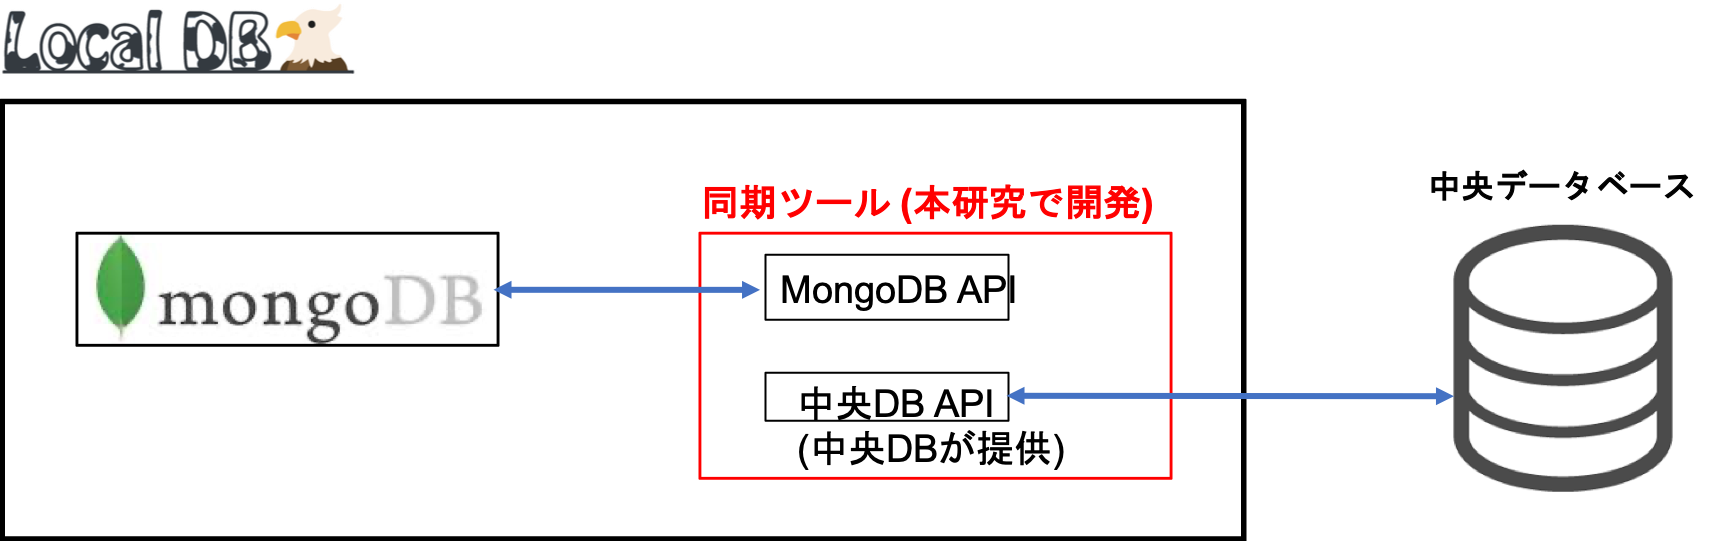
\includegraphics[width=13cm]{./interfacing_tools_system.png}
\caption[同期ツールのデータ通信のイメージ]{同期ツールのデータ通信のイメージ。本研究で開発を行っているのは図の赤線の領域に対応する同期ツールである。このツールはPythonを用いて開発しており、処理の中でローカルのMongoDBと通信するAPIと、中央データベースが開発、提供をしているAPIを用いることで、2つのデータベース間の同期を行っている。このとき、中央データベースとの通信はhttp通信で行われる。}
\label{interfacing_tools_system}
\end{figure}

特に本研究ではツールの枠組み設計に加えて、以下の機能を実装した。
\begin{itemize}
  \item モジュール及び構成するFEチップ情報のダウンロード機能
  \item 読み出し試験結果のアップロード機能
\end{itemize}

これらの機能のイメージを図\ref{interface_overview}に示す。
実装の詳細及び処理時間測定について8章で述べる。

\begin{figure}[bpt]\centering
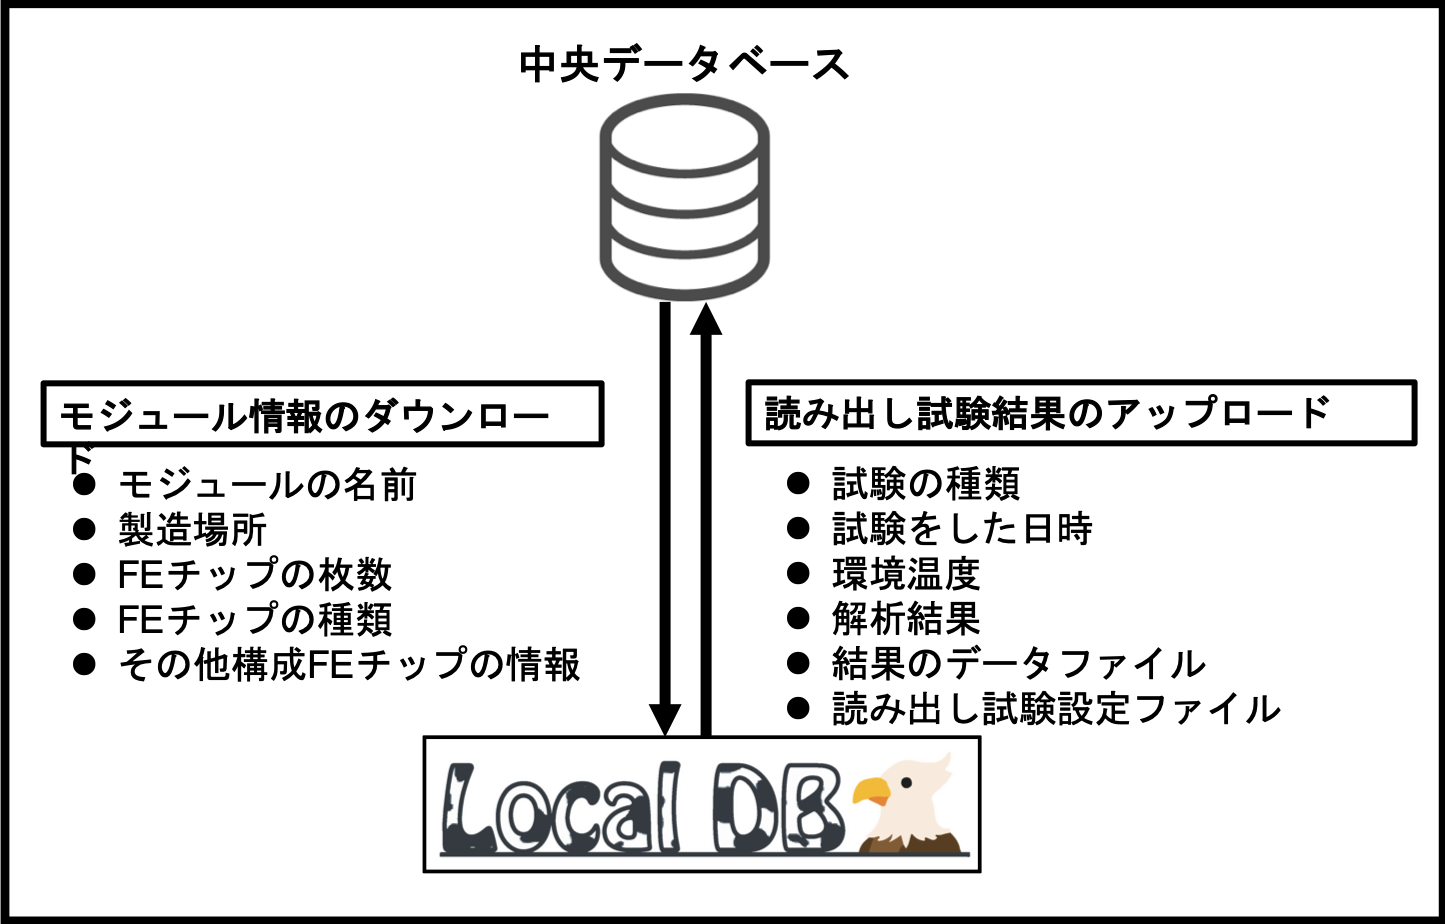
\includegraphics[width=11cm]{./interface_overview.png}
\caption[同期機能の概要]{同期機能の概要。本研究ではモジュール情報のダウンロードと読み出し試験結果のアップロード機能を実装した。図に示している情報を同期する機能となっている。}
\label{interface_overview}
\end{figure}

\clearpage
%%%%%%%%%%%%%%%%%%%%%%%%%%%%%%%%%%%%%%%%%%%%%%%%%%%
%%%%%%%%%%%%%%%%%%%%%%%%%%%%%%%%%%%%%%%%%%%%%%%%%%%
%%%%%%%%%%%%%%%%%%%%%%%%%%%%%%%%%%%%%%%%%%%%%%%%%%%

\subsection{ユーザ管理機能及び各種機能}

異常があった際に確認することを目的として、誰が試験を行ったかを記録することが必要である。
また、モジュールの登録や中央データベースとの同期など、データベースの機能使用を制限することも必要である。
これらを目的として、試験者及びデータベース使用者情報の管理システムを開発、実装した。
この詳細について以下に述べる。

\subsubsection{機能概要}
データベース権限の段階として、管理者、権限付きユーザ、一般ユーザの3段階を設けた。
各ユーザが使うことのできる機能を表\ref{user_functions_summary}に示す。

権限付きユーザの機能としてモジュール及び試験結果にコメント、タグをつける機能を実装した。使用したときの様子を図\ref{webapp_comment}、\ref{webapp_tag}に示す。

\subsubsection{ユーザ登録操作}
表\ref{user_functions_summary}において管理者と権限付ユーザの登録について説明する。

データベースシステム導入時に管理者のアカウントを作成する。
コマンドプロンプト上で開発したスクリプトを用いて実行することで管理者登録がなされ、この際ユーザ名とパスワードを入力する。

権限付ユーザについて、全ての品質試験者及びデータベースユーザ機能使用者は管理者によってユーザ登録される必要がある。
登録はウェブアプリケーションを用いて行い、以下の情報を入力する。
\begin{itemize}
  \item ユーザ名 
  \item 氏名
  \item 所属機関
  \item メールアドレス 
\end{itemize}

管理者が登録を完了すると、登録されたメールアドレスに登録完了メールと仮パスワードが届く。
このメールに従い、ウェブアプリケーション上でユーザがパスワード登録を完了する。

このようにメール機能を用いることでパスワード漏洩の防止、管理者操作の削減を目的としている。

\clearpage
%%%%%%%%%%%%%%%%%%%%%%%%%%%%%%%%%%%%%%%%%%%%%%%%%%%
%%%%%%%%%%%%%%%%%%%%%%%%%%%%%%%%%%%%%%%%%%%%%%%%%%%
%%%%%%%%%%%%%%%%%%%%%%%%%%%%%%%%%%%%%%%%%%%%%%%%%%%
\begin{table}[btp]
\begin{center}
\caption[ローカルデータベースユーザ権限及び使用機能一覧]{ローカルデータベースユーザ権限及び使用機能一覧。ローカルデータシステムにおけるユーザとして、管理者、権限付きユーザ、一般ユーザの3つを設けた。全てのユーザがウェブアプリケーションの閲覧をすることができる。管理者、権限付きユーザにはデータベース読み書き権限とウェブアプリケーションログイン権限が与えられ、試験結果のアップロード、アプリケーション上のユーザ機能の実行ができる。また管理者は権限付きユーザを登録することができる。}
\label{user_functions_summary}
  \small
  \begin{tabular}{|lll|} \hline
    ユーザ       & 付加される権限                               & 使用できる機能 \\ \hline
    管理者       & ユーザ管理権限                     & 権限付きユーザ登録機能\\ 
                 & データベース読み書き権限           & \\ 
                 & ウェブアプリケーションログイン権限 & \\ \hline
    権限付ユーザ & データベース読み書き権限           & 試験結果のアップロード\\ 
                 & ウェブアプリケーションログイン権限 & 中央データベースとのデータ同期機能\\ 
                 &                                    & その他ウェブアプリケーションの機能(コメント、タグ)\\ \hline
    一般ユーザ   &                                    & モジュール情報及び試験結果の閲覧 \\ \hline
  \end{tabular}
\end{center}
\end{table}

\begin{figure}[btp]\centering
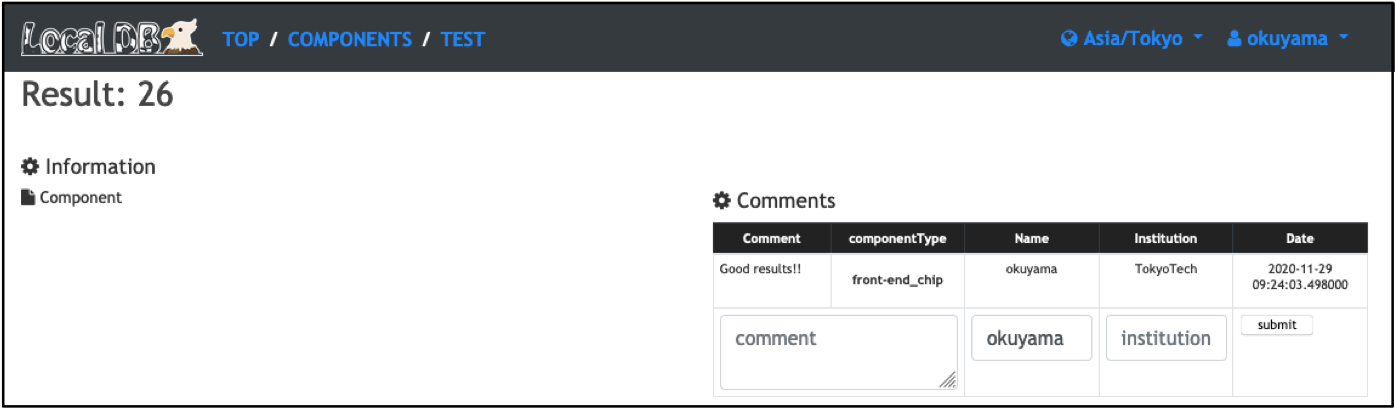
\includegraphics[width=12cm]{./viewer_comment.png}
\caption[ウェブアプリケーションにおけるコメント機能]{ウェブアプリケーションにおけるコメント機能。権限付きユーザ及び管理者はモジュールや試験結果に対してコメントをすることができる。図のようにページの右側にコメント欄があり、コメントをテキスト形式で記述することができる。}
\label{webapp_comment}
\end{figure}

\begin{figure}[bpt]\centering
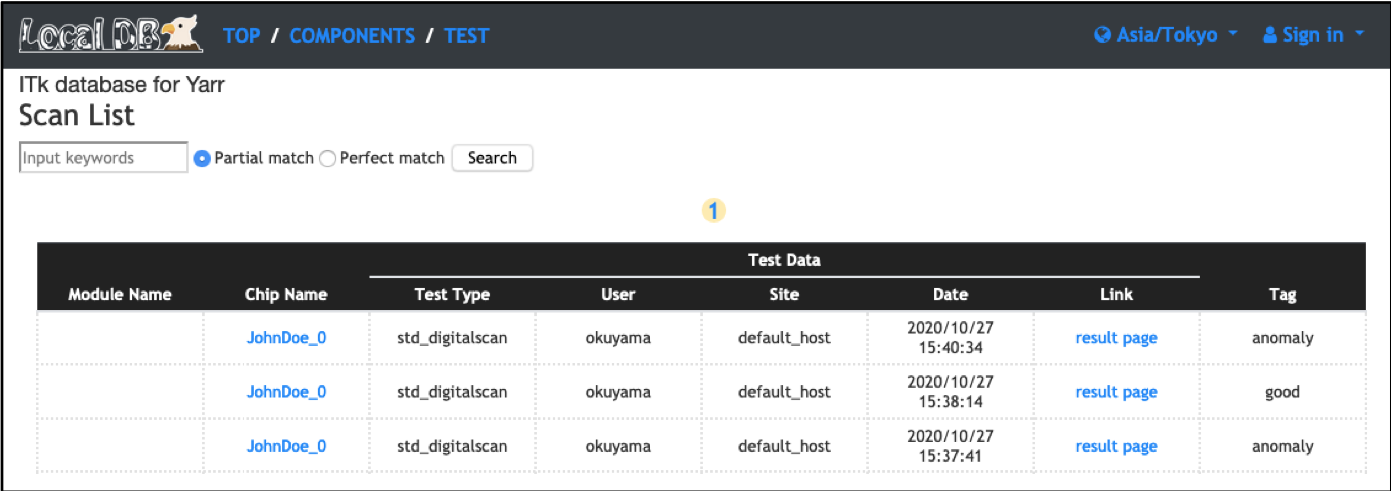
\includegraphics[width=12cm]{./viewer_tag.png}
\caption[ウェブアプリケーションにおけるタグ機能]{ウェブアプリケーションにおけるタグ機能。権限付きユーザ及び管理者はモジュールや試験結果に対してタグをつけることができる。図は試験結果の一覧ページであり、図の表において一番右の列がつけられたタグを示しており、図ではanomalyやgoodといったタグが付けられていることが分かる。}
\label{webapp_tag}
\end{figure}

\clearpage
%%%%%%%%%%%%%%%%%%%%%%%%%%%%%%%%%%%%%%%%%%%%%%%%%%%
%%%%%%%%%%%%%%%%%%%%%%%%%%%%%%%%%%%%%%%%%%%%%%%%%%%
%%%%%%%%%%%%%%%%%%%%%%%%%%%%%%%%%%%%%%%%%%%%%%%%%%%

\subsubsection{機能の仕組み}
ユーザ登録の際には内部で以下の2つの処理が行われるように実装した。

\begin{enumerate}
  \item MongoDBアカウントの作成、読み書き権限の付与
  \item ウェブアプリケーションで用いるユーザ情報ドキュメントの作成
\end{enumerate}

1の処理を行う理由は、登録ユーザが試験結果をmongoDBにアップロードできるようにするためである。
2の情報は、ウェブアプリケーション内でのログイン判断、ユーザの情報保持に使う。
この情報は表\ref{localdb_structure}のviewer.userに保存される。
2つの処理について、実際に保存されるドキュメントの例をリスト\ref{user_doc_1}、\ref{user_doc_2}以下に示す。

\begin{lstlisting}[basicstyle=\scriptsize,caption=MongoDBアカウント情報を持つドキュメントの例。リスト中の"roles"より、localdbとlocaldbtoolsの読み書き権限が付加されていることが分かる。,label=user_doc_1]
{
	"_id" : "localdb.hokuyama",
	"userId" : UUID("fee321eb-83b8-434a-a4a0-fff638b5db36"),
	"user" : "hokuyama",
	"db" : "localdb",
	"credentials" : {
    ...
	},
	"roles" : [
		{
			"role" : "readWrite",
			"db" : "localdb"
		},
		{
			"role" : "readWrite",
			"db" : "localdbtools"
		}
	]
}
\end{lstlisting}

\begin{lstlisting}[basicstyle=\scriptsize,caption=ウェブアプリケーションで扱うユーザ情報を持つドキュメントの例。リスト\ref{user_doc_1}で示したものとは別に、ウェブアプリケーション内でユーザ情報を扱うためにこのドキュメントを保持する必要がある。ウェブにおいてログインはこのドキュメントの存在確認をもってなされる。パスワードはhash化して保存している。,label=user_doc_2]
{
	"_id" : ObjectId("5f0bbe84ef87af2628865de7"),
	"sys" : {
		"rev" : 0,
		"cts" : ISODate("2020-07-13T10:53:07.943Z"),
		"mts" : ISODate("2020-07-13T10:53:07.943Z")
	},
	"username" : "hokuyama",
	"name" : "Hiroki Okuyama",
	"auth" : "readWrite",
	"institution" : "Tokyo Institute of Technology",
	"Email" : "okuyama@hep.phys.titech.ac.jp",
	"password" : "5f4dcc3b5aa765d61d8327deb882cf99"
}
\end{lstlisting}

\clearpage
%%%%%%%%%%%%%%%%%%%%%%%%%%%%%%%%%%%%%%%%%%%%%%%%%%%%%%%
%%%%%%%%%%%%%%%%%%%%%%%%%%%%%%%%%%%%%%%%%%%%%%%%%%%
%%%%%%%%%%%%%%%%%%%%%%%%%%%%%%%%%%%%%%%%%%%%%%%%%%%%%%%
\newpage
\subsection{品質試験結果の登録と組み立て工程の自動更新}
ローカルデータベースへアップロードした品質試験結果の中から、本結果として中央データベースへアップロードする結果を選択する機能を開発した。
品質試験は各モジュール、各組み立て工程に対して行うものであるため、結果選択も同様に工程毎に行うことを想定している。
結果選択後、データベースにおける組み立て工程の情報は次のものへ自動的に更新する機能となっている。

\subsubsection{概要}
あるモジュール、組み立て工程に対して結果を選択する様子を図\ref{webapp_sign_off}に示す。組み立て工程も自動更新されていることがわかる。

\subsubsection{仕組み}
リスト\ref{qc_status}、\ref{qc_module_status}のようなドキュメントを作成、保存する。
リスト\ref{qc_status}は全てのモジュールに対して共通のドキュメントであり、組み立て工程と各工程における品質試験項目を記録する。
これらの情報は中央データベースより取得される。
この情報を参照することでローカルデータベース内部での組み立て工程の管理が可能となっている。

リスト\ref{qc_module_status}は各モジュールに対して1つ存在し、以下のような情報を保持する。
\begin{itemize}
  \item 現在工程
  \item 各工程における品質試験結果のID
\end{itemize}


\begin{lstlisting}[basicstyle=\scriptsize,caption=組み立て工程及び品質試験一覧情報ドキュメント。このようなドキュメントを作成、保持しておくことで組み立て工程及び品質試験の情報を扱う。ローカルデータベース内に1つこのドキュメントを保持し、品質試験結果選択、組み立て工程の更新時にこのドキュメントを参照する。このドキュメントは中央データベースよりデータ取得して作成する。,label=qc_status]
{
	"_id" : ObjectId("5fc89aa232d56b29091fd64d"),
	"sys" : {
		"mts" : ISODate("2020-12-03T07:58:26.310Z"),
		"cts" : ISODate("2020-12-03T07:58:26.310Z"),
		"rev" : 0
	},
	"dbVersion" : 1.01,
	"proddbVersion" : 1.01,
	"stage_flow" : [
		"MODULETOPCB",
		"MODULEWIREBONDING",
		"MODULEWIREBONDPROTECTION",
		"MODULEPARYLENECOATING",
		"MODULETHERMALCYCLING",
		"MODULEBURNIN",
		"MODULERECEPTION"
	],
	"stage_test" : {
		"MODULETOPCB" : [
			"OPTICAL",
			"GLUE_MODULE_FLEX_ATTACH",
			"MASS",
			"METROLOGY"
		],
		"MODULEWIREBONDING" : [
			"WIREBONDING",
			"OPTICAL",
			"SENSOR_IV",
			"PIXEL_FAILURE_TEST",
			"SLDO_VI",
			"WIREBOND",
			"CHIP_CONFIGURATION"
		],
		"MODULEWIREBONDPROTECTION" : [
			"OPTICAL",
			"POTTING",
			"MASS",
			"READOUT_IN_BASIC_ELECTRICAL_TEST",
			"SENSOR_IV",
			"REGISTER_TEST"
		],
    ...
	},
...
}
\end{lstlisting}

\begin{lstlisting}[basicstyle=\scriptsize,caption=モジュールの組み立て工程及び品質試験結果管理のためのドキュメント例。各モジュールにおいて現在の組み立て工程及び選択された品質試験結果がこのドキュメントに保存される。ドキュメント内の"currentStage"に現工程を保持する。また選択した試験結果のIDを"QC$\_$results"に各組み立て工程ごとに持つようになっている。,label=qc_module_status]
{
	"_id" : ObjectId("5fc4be4c12a45922a91b0e75"),
	"sys" : {
		"mts" : ISODate("2020-11-30T09:41:32.411Z"),
		"cts" : ISODate("2020-11-30T09:41:32.411Z"),
		"rev" : 0
	},
	"dbVersion" : 1.01,
	"proddbVersion" : 1.01,
	"component" : "5fa79114e615fa000a1a5976",
	"currentStage" : "MODULEWIREBONDPROTECTION",
	"latestSyncedStage" : "MODULEWIREBONDING",
	"status" : "created",
	"rework_stage" : [ ],
	"QC_results" : {
		"MODULETOPCB" : {
			"OPTICAL" : "5fc4c2cfb6c93d451e2c9ac1",
			"GLUE_MODULE_FLEX_ATTACH" : "-1",
			"MASS" : "5fc4c2da27766dc6e89c024f",
			"METROLOGY" : "5fc4c2eaf1f19d9cb5859f00"
		},
		"MODULEWIREBONDING" : {
			"WIREBONDING" : "-1",
			"OPTICAL" : "5fc4c4c8b7d0c86912b4958f",
			"SENSOR_IV" : "5fc4c59e9e283a57ccaa1088",
			"PIXEL_FAILURE_TEST" : "5fca342f6e9f1f5eafedfb92",
			"SLDO_VI" : "-1",
			"WIREBOND" : "-1",
			"CHIP_CONFIGURATION" : "-1"
		},
		"MODULEWIREBONDPROTECTION" : {
			"OPTICAL" : "-1",
			"POTTING" : "-1",
			"MASS" : "-1",
			"READOUT_IN_BASIC_ELECTRICAL_TEST" : "-1",
			"SENSOR_IV" : "-1",
			"REGISTER_TEST" : "-1"
		},
    ...
	}
}
\end{lstlisting}

\begin{figure}[bpt]\centering
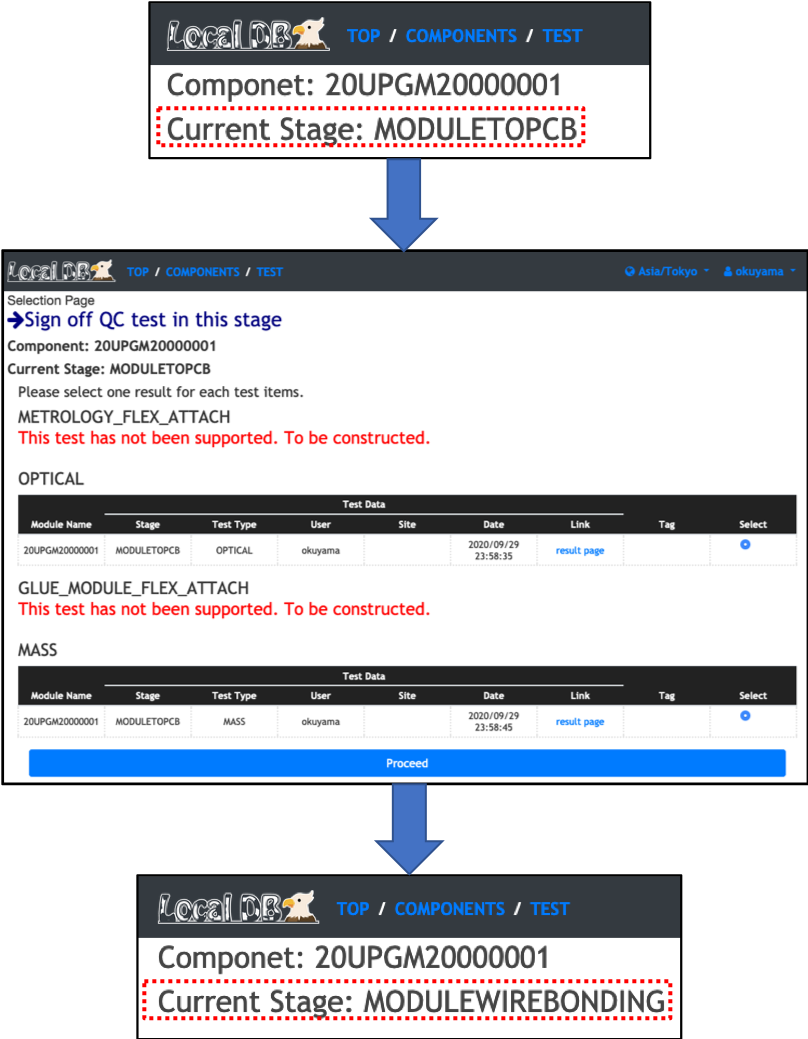
\includegraphics[width=14cm]{./webapp_sign_off.png}
\caption[結果選択画面及び組み立て工程表示の例]{結果選択画面及び組み立て工程表示の例。図の上部で組み立て工程が"MODULETOPCB"である。この段階において結果を選択する処理を行うとローカルデータベース内で選択された結果にタグ付けがなされる。図の中部においてその処理を行なっており、この図では"OPTICAL"と"MASS"の結果を選択している。選択した結果は中央データベースと同期される。また結果選択後は組み立て工程が自動的に更新される。図の下部では"MODULEWIREBONDING"になっていることが分かる。}
\label{webapp_sign_off}
\end{figure}

\clearpage
%%%%%%%%%%%%%%%%%%%%%%%%%%%%%%%%%%%%%%%%%%%%%%%%%%%%%%%
%%%%%%%%%%%%%%%%%%%%%%%%%%%%%%%%%%%%%%%%%%%%%%%%%%%%%%%

\newpage
\subsection{読み出し試験結果におけるピクセル解析ツール}
節\ref{sec:pixel_analysis}で述べたように、読み出し試験ではピクセル解析を行う。
これを円滑に行うために、ピクセル解析ツールを開発した。また開発した解析ツールをローカルデータベースシステムに組み込んだ。
このツールについての詳細を以下に示す。

\subsubsection{概要}
YARRで読み出し試験を行った場合、結果ファイル及びディレクトリは各試験項目ごとにわかれて生成される。
また各結果ファイルにはモジュール上の全ピクセル結果がJSONの形で保存されている。

一方、ピクセル解析において、いくつかの試験結果を統一的に扱い、各ピクセルごとに解析を行う必要がある。
そこで、開発した解析ツールでは複数の結果ファイルを1つに統合し、ピクセルごとの解析処理を単純化する役割を担っている。
開発にはPythonとC++を用いた。またCERNが提供している解析フレームワークであるROOT\cite{4-5}を使用し、いくつかの試験データの統一ファイルとして、ROOT内部機能であるTreeを使用した。
このファイル統合処理のイメージを図\ref{analysis_tool_motivation}に示す。

\begin{figure}[bpt]\centering
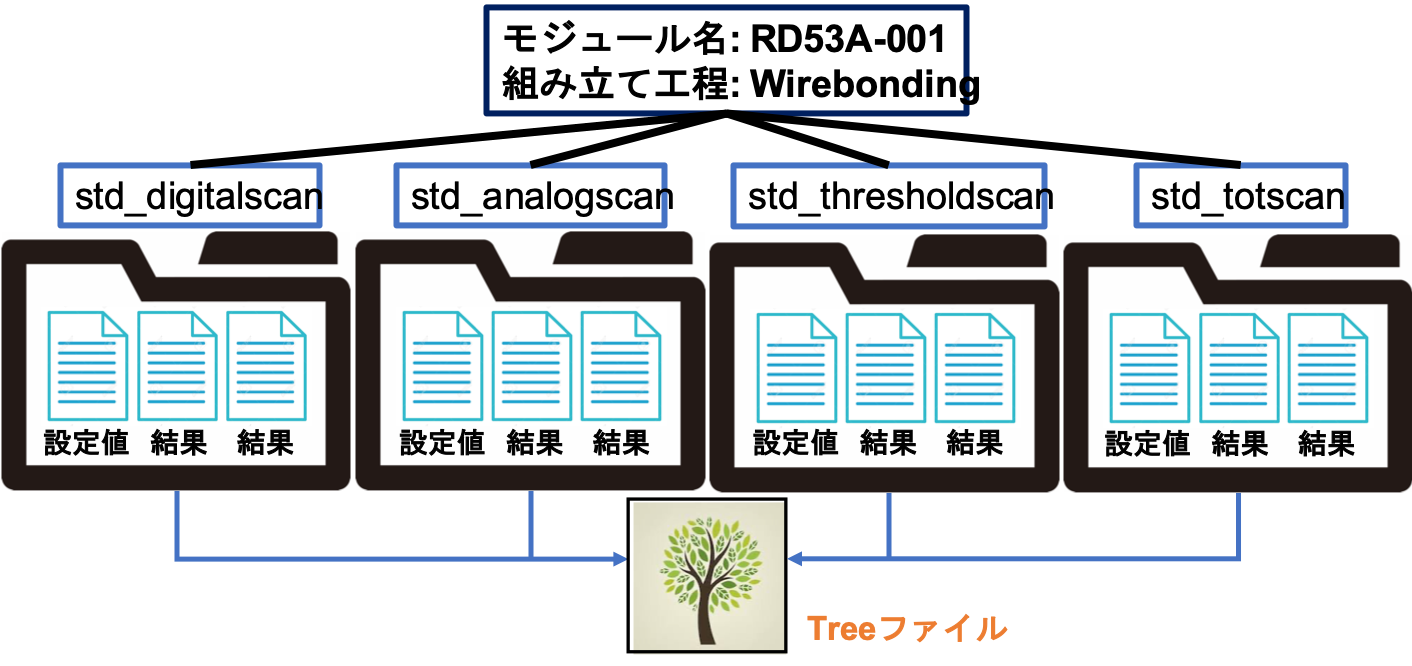
\includegraphics[width=12cm]{./analysis_tool_motivation.png}
\caption[ピクセル解析ツールにおけるファイル統合処理のイメージ]{ピクセル解析ツールにおけるファイル統合処理のイメージ。YARRの出力ファイル及びディレクトリは\texttt{std$\_$digitalscan}や\texttt{std$\_$thresholdscan}というように読み出し項目ごとである。ピクセル解析ツールでは、図のようにあるモジュールに関連する結果ファイルを統合し、ピクセルごとに行う解析処理を簡易化する狙いがある。}
\label{analysis_tool_motivation}
\end{figure}

実際に作ったTreeファイルと、データ構造のイメージを図\ref{analysis_tool_tree}に示す。

\begin{figure}[bpt]
  \begin{minipage}{0.4\hsize}
    \begin{center}
    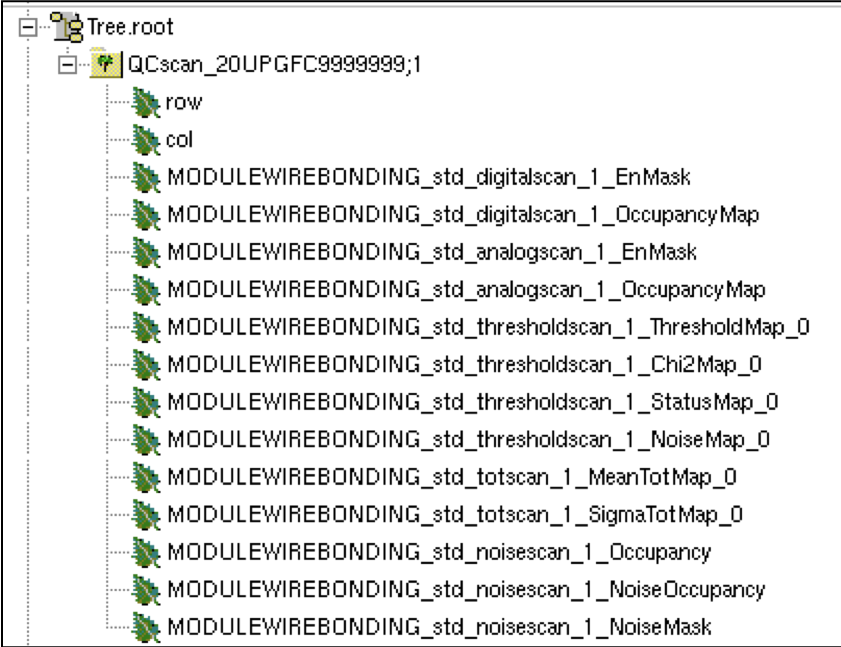
\includegraphics[width=6cm]{./analysis_tool_tree_file.png}
    \end{center}
  \end{minipage}
  \begin{minipage}{0.4\hsize}
    \begin{center}
    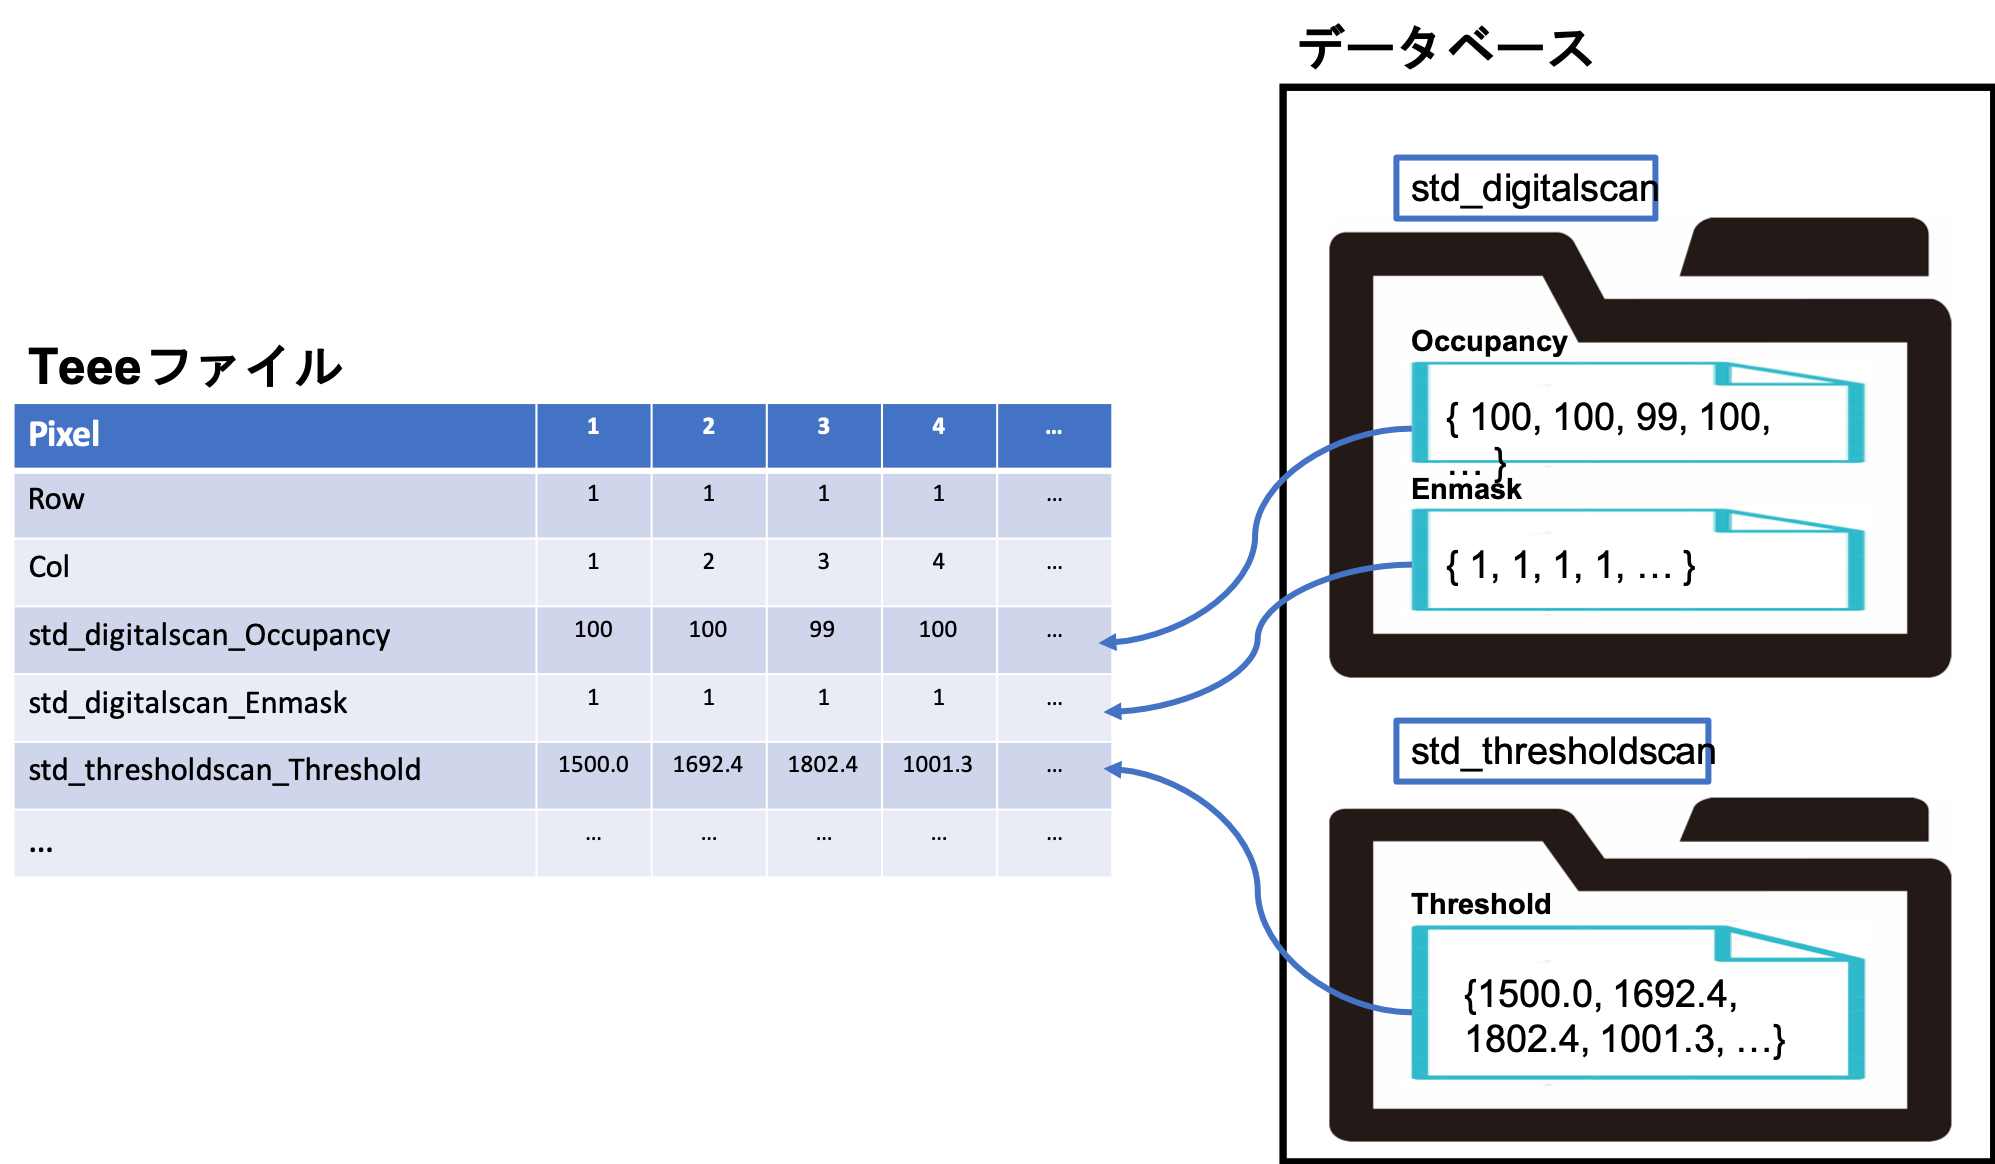
\includegraphics[width=8cm]{./analysis_tool_tree_image.png}
    \end{center}
  \end{minipage}
  \caption[Treeファイルとそのデータ保持]{Treeファイルとそのデータ保持。実際にこのツールを用いて作ったTreeファイルの内部構造の様子(左)とそのデータ保持のイメージ(右図)を示す。Treeファイルでは、右図のように1つの表に試験結果をまとめている。各行が\texttt{std$\_$digitalscan}といった各読み出し項目に対応し、各列が1ピクセルに対応する。モジュール上の行列(Row、Col)の番号を表の上部に持っておくことで、モジュール上におけるピクセルの位置情報を保持する。}
  \label{analysis_tool_tree}
\end{figure}

\subsubsection{ツールの内部構造と処理の流れ}
開発したツールは、主に以下で説明する3つの実行ファイルで構成される。それぞれの役割について説明する。

\begin{description}
  \item[getData.py (Python)]\mbox{}\\ 
    データベースから対象となるデータファイルを取得、キャッシュファイルとしてサーバー上の一時ディレクトリに保存.
  \item[makeTree (C++)]\mbox{}\\ 
    getData.pyを用いて生成されたキャッシュファイルを読み込み、Treeファイルを作成.
  \item[analysis (C++)]\mbox{}\\ 
  作成したTreeファイルを読み込みピクセル解析を実行、結果値やプロットを出力.
\end{description}

処理の流れのイメージを図\ref{analysis_tool_flow}に示す。
データベースとの通信に関してはMongoDBや現システムとの親和性を考慮し、Pythonを使用した。
Treeファイル作成やその後の解析処理のスクリプトは、ROOTを使用する観点からC++を使用した。
またピクセル解析以外の解析に対しても適応可能とするため、Tree作成部と解析処理部のファイルは分割した。

\begin{figure}[bpt]\centering
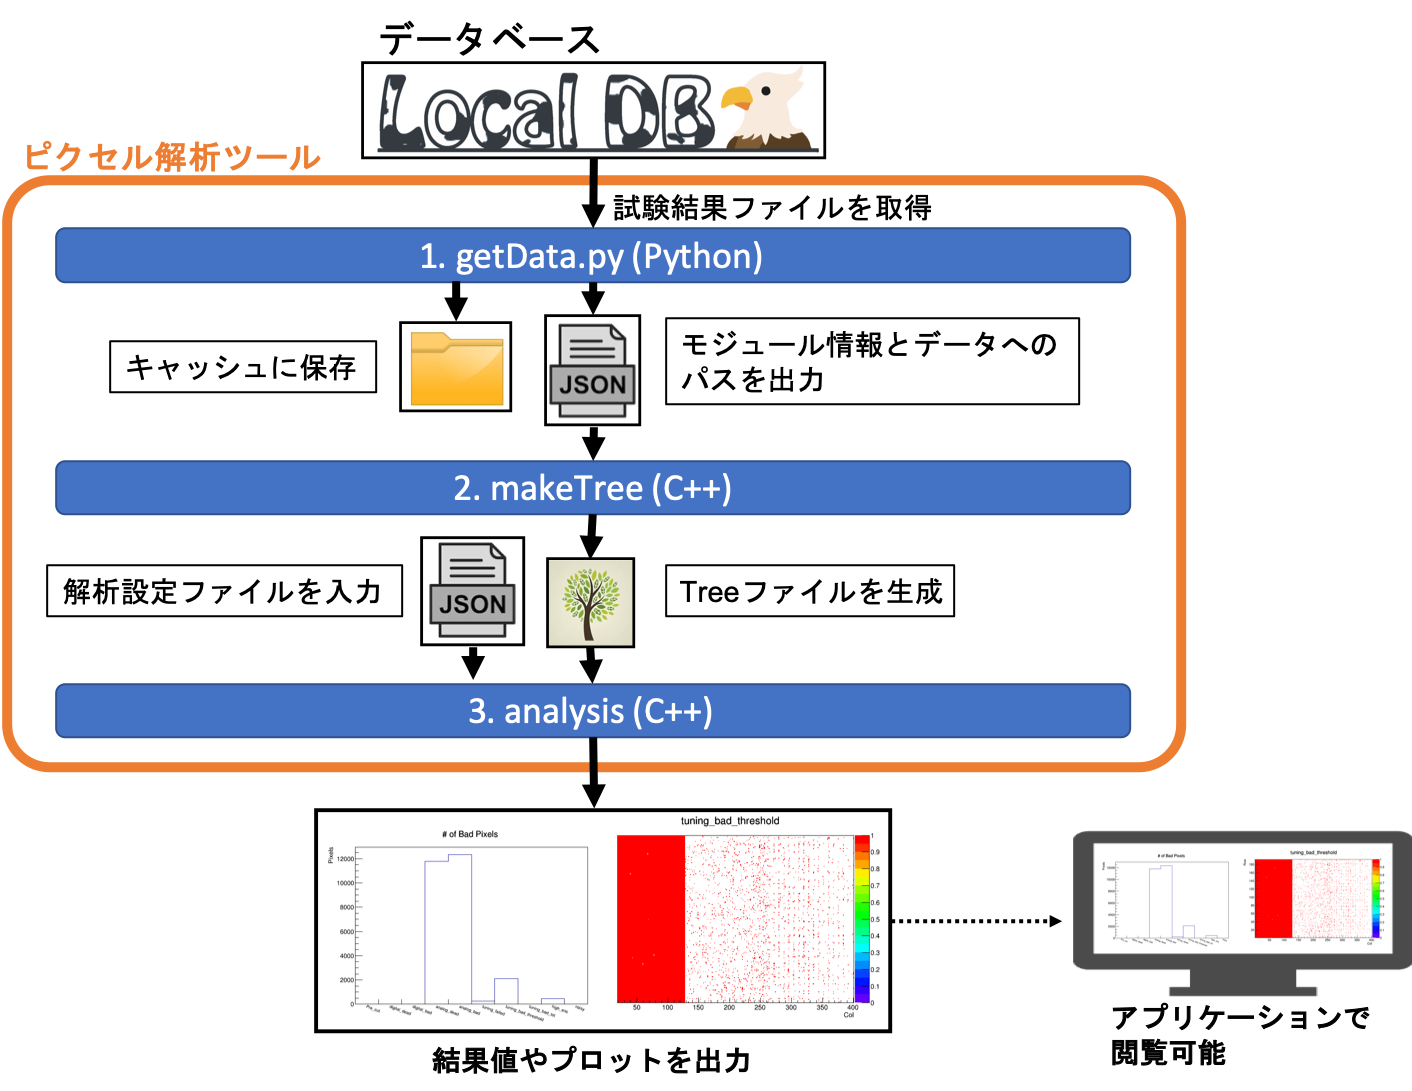
\includegraphics[width=10cm]{./analysis_tool_flow.png}
\caption[ピクセル解析ツールの処理の流れ]{ピクセル解析ツールの処理の流れ。ピクセル解析ツールは、図のように3つの実行ファイルにより構成される。getData.py(Python)にてデータベースから結果の取得を行い、makeTree(C++)にてTreeファイルの作成、analysis(C++)にてピクセル解析及び結果のプロットが出力される。}
\label{analysis_tool_flow}
\end{figure}

\clearpage
%%%%%%%%%%%%%%%%%%%%%%%%%%%%%%%%%%%%%%%%%%%%%%%%%%%%%%%
%%%%%%%%%%%%%%%%%%%%%%%%%%%%%%%%%%%%%%%%%%%%%%%%%%%%%%%
%%%%%%%%%%%%%%%%%%%%%%%%%%%%%%%%%%%%%%%%%%%%%%%%%%%
\subsection{読み出し試験結果の検索機能}
登録モジュールや品質試験結果の一覧ページに検索機能を実装した。
確認したいモジュール情報や試験結果を迅速に取得し、閲覧できることを目的としている。検索機能を使用している様子を図\ref{webapp_search_function}に示す。

キーワードを入力し、検索することができる仕組みとなっていて、一般的なウェブページの検索エンジンのように扱うことができる。
生産に向けて、検索にかかる処理時間測定を行った。検索機能実装方法の詳細と処理時間についての詳細は、6章で述べる。
現在は単一キーワード検索の他に、以下の機能を実装している。
\begin{itemize}
  \item 完全一致、部分一致検索
  \item AND、OR検索
\end{itemize}

\begin{figure}[bpt]\centering
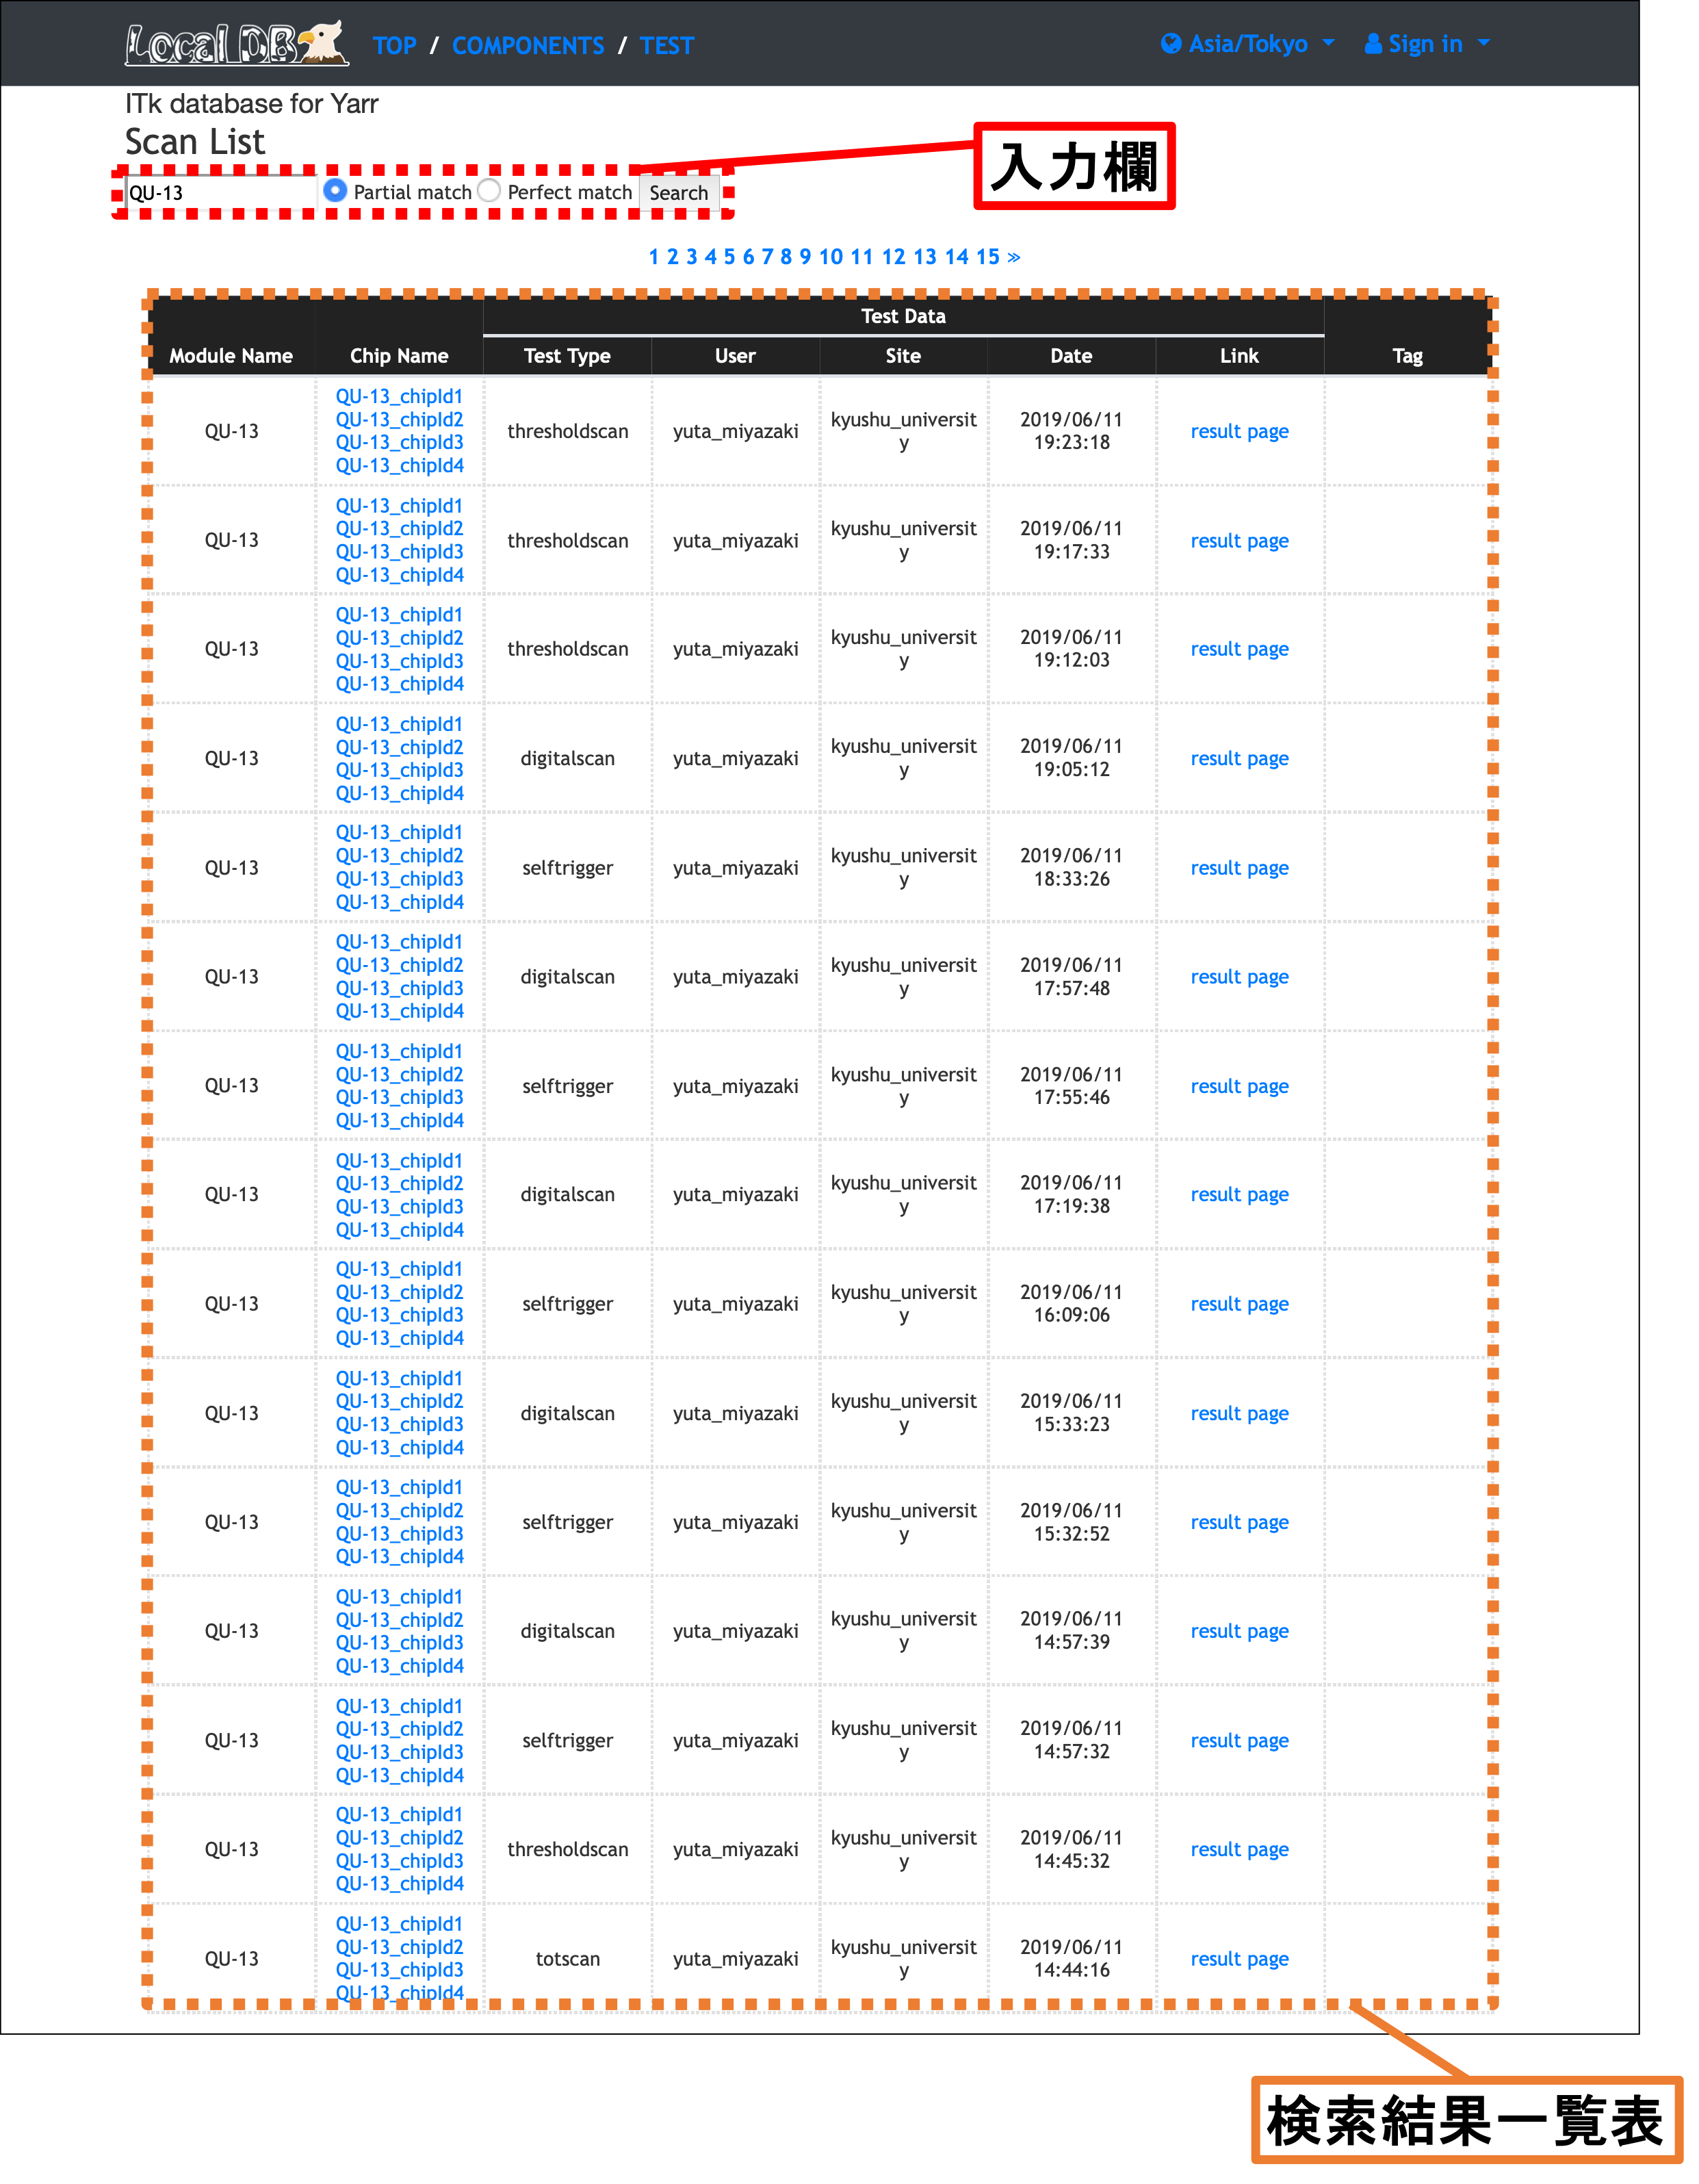
\includegraphics[width=10.5cm]{./webapp_search_function.png}
\caption[ウェブアプリケーションにおける検索機能の様子]{ウェブアプリケーションにおける検索機能の様子。図は検索結果一覧表示のページである。図の上部に入力欄があり(赤破線)、ここにキーワードを入力し検索を実行する。図の例では"QU-13"と入力しており、検索結果にはモジュール名QU-13の試験結果が一覧表示されていることが分かる。}
\label{webapp_search_function}
\end{figure}


\clearpage
%%%%%%%%%%%%%%%%%%%%%%%%%%%%%%%%%%%%%%%%%%%%%%%%%%%%%%%
%%%%%%%%%%%%%%%%%%%%%%%%%%%%%%%%%%%%%%%%%%%%%%%%%%%%%%%
%%%%%%%%%%%%%%%%%%%%%%%%%%%%%%%%%%%%%%%%%%%%%%%%%%%%%%%
\subsection{量産時におけるデータベース操作の流れの確立}
量産時におけるデータベース操作の流れを確立した。
以下に従い、モジュール組み立て時におけるデータ管理がなされる。
\begin{enumerate}
  \item 中央データベースへモジュール登録及び登録情報のダウンロード
  \item 1で登録したモジュールに対して品質試験結果のローカルデータベースへのアップロード
  \item ステージ毎に品質試験結果の登録と中央データベースへアップロード
\end{enumerate}

流れのイメージを図\ref{dbsystem_flow}に示す。
品質試験結果のアップロードは各組み立て工程毎に行う。ローカルデータベースで品質試験結果を組み立て工程毎にまとめて扱い、各モジュールの現組み立て工程を正確に管理する目的がある。
\begin{figure}[bpt]\centering
  \begin{minipage}{0.5\hsize}
    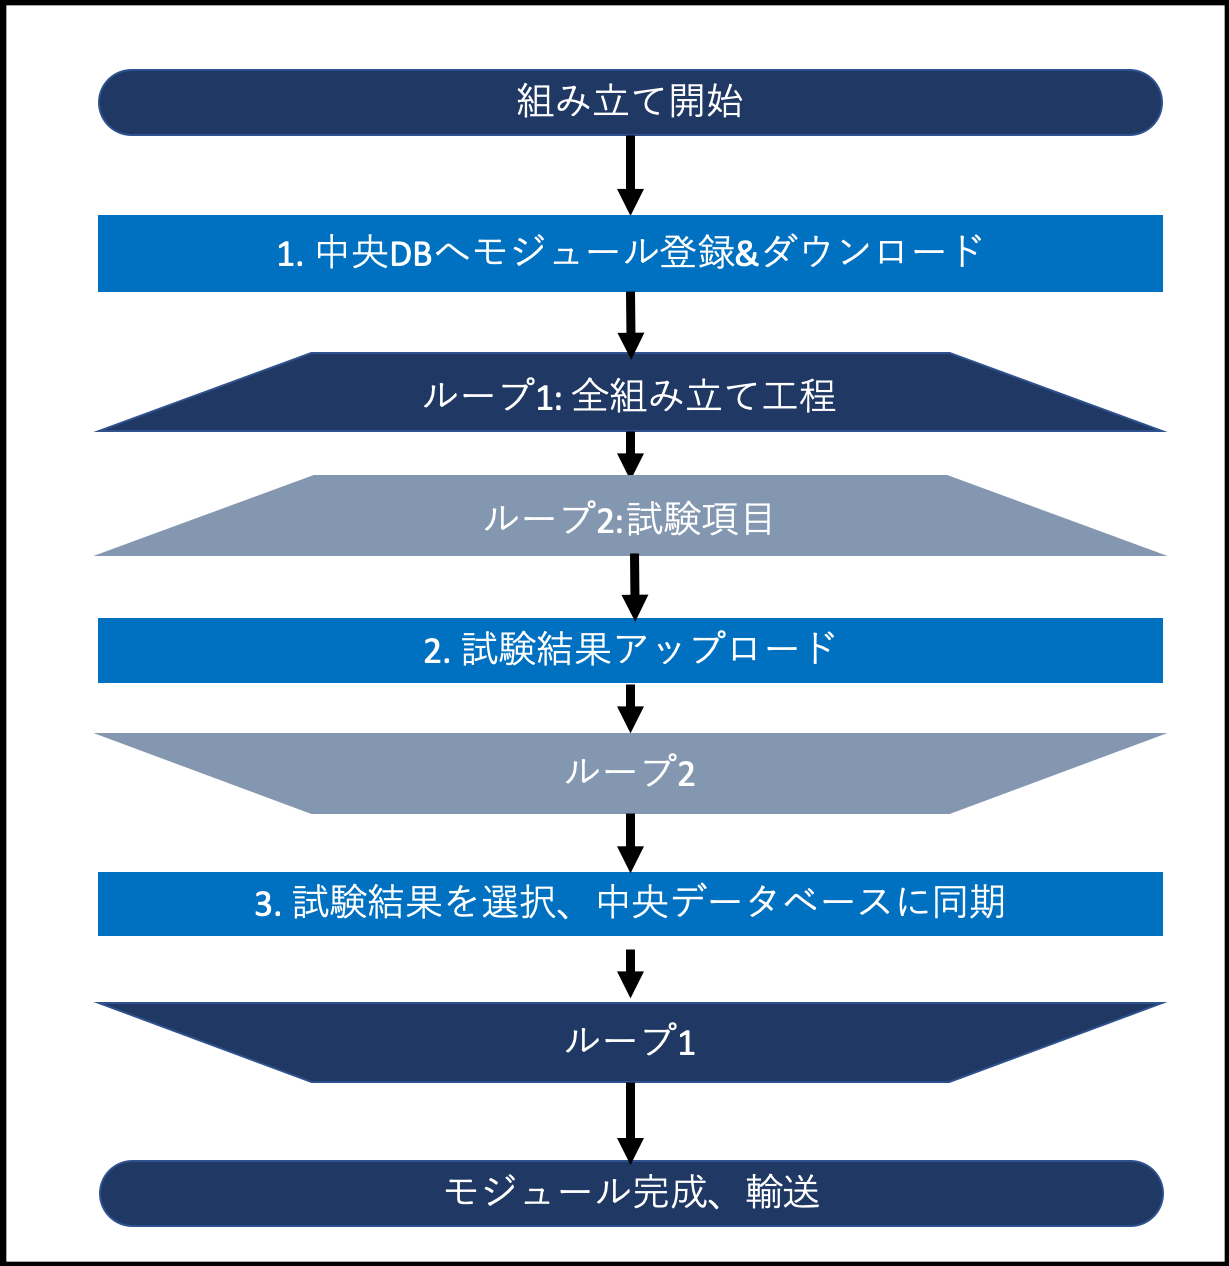
\includegraphics[width=7cm]{./dbsystem_flowchart.png}
  \end{minipage}
  \begin{minipage}{0.4\hsize}
    \includegraphics[width=5cm]{./dbsystem_flow_image.png}
  \end{minipage}
\caption[各モジュールにおけるデータベースシステム操作の流れ]{各モジュールにおけるデータベースシステム操作の流れ。モジュール組み立てにおけるデータベース操作の初めに、中央データベースにモジュール登録及びローカルデータベースへモジュール情報のダウンロードを行う(処理1)。その後、ダウンロードしたモジュールに対して組み立て工程に応じた試験結果を生成、ローカルデータベースに保存する(処理2)。各組み立て工程の終わりに試験結果の選択を行い、中央データベースに試験結果を同期する(処理3)。}
\label{dbsystem_flow}
\end{figure}

全組み立て工程が終了すると、モジュールの情報及び品質試験結果が全て中央データベースへ同期されている状態となる。


この品質試験におけるデータベース操作の流れの確立に向けて、2月にCERNに行なったシステムチュートリアルで操作の流れを試験した。ユーザに対する操作の流れの周知と機能確認を行うことができた。チュートリアルの概要は付録\ref{cap:appA}に記す。
またシステムのドキュメント\cite{4-7}を作成し、その中に具体的なデータベース操作の流れを記述している。量産時に各機関が適切な流れでデータ管理をできるようにした。


データベース操作の流れの試験として、実際に品質試験のデモンストレーションを行い、各機能が正常に動作するのかの確認を行なった。
詳細を5章で述べる。


\chapter{品質試験項目:読み出し試験に用いるソフトウェアと学内実験室におけるデモンストレーション}

\section{読み出し試験に用いるソフトウェアの概要}

\section{読み出し試験結果解析ツールの開発}

\section{学内実験室におけるデモンストレーション}
学内実験室で開発しているソフトウェアを用いて読み出し試験を行い、実際の生産時における流れのデモンストレーションを局所的に行なった。
その詳細について以下に示す。

\subsection{デモンストレーションの流れ}

今回のデモンストレーションで確認した機能を以下に示す。
\begin{itemize}
  \item 中央データベースとローカルデータベースのデータ同期機能(モジュールIDのダウンロード、試験結果のアップロード)
  \item 読み出し試験に使う各種機能(設定ファイル生成、温度、電圧、電流モニタリング、試験結果閲覧)
  \item 結果選択とピクセル解析機能
\end{itemize}

またデモンストレーションにおける流れの概要を図\ref{demo_flow}に示す。

\begin{figure}[bpt]\centering
\includegraphics[width=1cm]{figure}
\caption[デモンストレーションの流れ]{デモンストレーションの流れ}
\label{demo_flow}
\end{figure}

\subsection{読み出し試験セットアップ}
読み出し試験に用いるハードウェアのセットアップを表\ref{readout_setup_table}、概要を図\ref{readout_setup_overview}、各ハードウェアの写真を\ref{readout_setup_picture}に示す。
各装置の詳細については付録Bに示す。

\begin{table}[tbp]
\begin{center}
\caption[各ハードウェアの性能]{各ハードウェアの性能}
\label{readout_setup_table}
  \begin{tabular}{|ll|} \hline
    1 & 2 \\ \hline
    result 1 & result 2 \\ \hline 
  \end{tabular}
\end{center}
\end{table}

\begin{figure}[bpt]\centering
\includegraphics[width=1cm]{figure}
\caption[ハードウェアセットアップの概要]{ハードウェアセットアップの概要}
\label{readout_setup_overview}
\end{figure}

\begin{figure}[bpt]\centering
\includegraphics[width=1cm]{figure}
\caption[各ハードウェアの写真]{各ハードウェアの写真}
\label{readout_setup_picture}
\end{figure}

\subsection{読み出し試験内容}
読み出し試験を通して、モジュールに与える電圧値、電流値、チップ横についているNTCから読み取れる温度を記録した。
以下の流れに沿って読み出しを行なった。

\subsection{機能確認}
\subsubsection{モジュールIDのダウンロード}
登録したモジュールのIDを機能を使ってダウンロードし、ウェブアプリケーションで確認した。
確認した画面を図\ref{download_SCC}に示す。

\begin{figure}[bpt]\centering
\includegraphics[width=1cm]{figure}
\caption[ダウンロードしたモジュールID確認画面]{ダウンロードしたモジュールID確認画面}
\label{download_SCC}
\end{figure}

\subsubsection{読み出し試験}
以下の流れで読み出し試験を行なった。読み出し試験はサーバーのシェルを用いて行う。

・設定ファイル生成

ダウンロードしたモジュールのIDを用いて、読み出しに用いる設定ファイルを生成した。
イメージを図\ref{config_retriever}、実際に生成したファイルを確認した画面を図\ref{create_config}に示す。

\begin{figure}[bpt]\centering
\includegraphics[width=1cm]{figure}
\caption[設定ファイル生成のイメージ]{設定ファイル生成のイメージ}
\label{config_retriever}
\end{figure}

\begin{figure}[bpt]\centering
\includegraphics[width=1cm]{figure}
\caption[生成ファイル確認画面]{生成ファイル確認画面}
\label{create_config}
\end{figure}

・試験実施とアップロード

上述した流れに沿って読み出し試験を実施した。試験結果は各試験の終わりに自動的にアップロードされるようなシステムとなっている。

・電圧値、電流値、温度のモニタリング

記録した値をGrafanaを使ってモニタリングをした。その様子を図\ref{monitoring_dcs}に示す。

\begin{figure}[bpt]\centering
\includegraphics[width=1cm]{figure}
\caption[DCSのモニタリング]{DCSのモニタリング}
\label{monitoring_dcs}
\end{figure}

・試験結果の閲覧

ウェブアプリケーションを用いて、試験結果を閲覧した。その様子を図\ref{view_scan_result}、\ref{view_dcs}に示す。

\begin{figure}[bpt]\centering
\includegraphics[width=1cm]{figure}
\caption[試験結果の閲覧]{試験結果の閲覧}
\label{view_scan_result}
\end{figure}

\begin{figure}[bpt]\centering
\includegraphics[width=1cm]{figure}
\caption[各測定値の閲覧]{各測定値の閲覧}
\label{view_dcs}
\end{figure}

各scanの結果を\ref{scan_result}に示す。

\begin{figure}[bpt]\centering
\includegraphics[width=1cm]{figure}
\caption[各scan結果]{各scan結果}
\label{scan_result}
\end{figure}

\subsubsection{結果選択とピクセル解析}
読み出し結果を選択し、ピクセル解析を行なった。結果選択の様子を図\ref{select_scans}、解析結果を表\ref{pixel_analysis_result}に示す。

\begin{figure}[bpt]\centering
\includegraphics[width=1cm]{figure}
\caption[scan結果選択の様子]{scan結果選択の様子}
\label{select_scans}
\end{figure}

\begin{table}[tbp]
\begin{center}
\caption[ピクセル解析結果]{ピクセル解析結果}
\label{pixel_analysis_result}
  \begin{tabular}{|ll|} \hline
    1 & 2 \\ \hline
    result 1 & result 2 \\ \hline 
  \end{tabular}
\end{center}
\end{table}

\subsubsection{試験結果アップロード}
選択した結果を中央データベースにアップロードし、各ファイルが正しくアップロードされていることを確認した。
各ファイルの存在を確認した結果を表\ref{scan_upload_pd}に示す。

\begin{table}[tbp]
\begin{center}
\caption[scan fileの存在確認]{scan fileの存在確認}
\label{pixel_analysis_result}
  \begin{tabular}{|ll|} \hline
    1 & 2 \\ \hline
    result 1 & result 2 \\ \hline 
  \end{tabular}
\end{center}
\end{table}

\subsubsection{今後の開発方針}

生産の本番に向けて、中央データベースにあげるデータを再検討する必要がある。
現在のシステムでは5つの試験に対して結果ファイルだけをあげるものとなっている。
情報としては不十分であり、以下のような項目を検討しアップロード情報として付け加えることが必要であり、今後の課題となっている。

\begin{itemize}
  \item DCSの情報
  \item 適切な読み出し試験項目
  \item ピクセル解析の結果
\end{itemize}


\chapter{ローカルデータベースにおける読み出し試験結果検索機能の詳細と処理時間測定}

生産時には、読み出し試験の結果は一つの機関で大量に生じるものである。
4章で述べたように、任意のタイミングで必要な結果を取得できる検索機能を実装した。詳細について以下に示す。


\section{実装方法}
今回の実装では、一般的にウェブで用いられているフリーワードの検索エンジンのような機能を実装しようと考えた。
ユーザの操作を最小限にし、柔軟な検索ができるようにするためである。

読み出し試験において、対象とする検索キーワードを以下の項目に絞った。
システムにおいて、アップロードされた試験結果に関わるデータベース内の情報は固定されていて、試験結果情報の変更はしないことを前提としている。
そのため、ユーザが対象としたい検索キーワードは以下の項目に限られ、検索キーワードとして以下の項目をサポートすれば十分であると考えた。

\begin{itemize}
  \item モジュール及びFEチップのID
  \item 読み出し試験項目(例:std$\_$digitalscan)
  \item 読み出し試験者
  \item 読み出し試験場所
  \item 試験日時(将来的に範囲指定を用いた検索機能を検討)
  \item タグ機能を用いてつけられたタグ
\end{itemize}

そこで実装方法として、以下の2つを考えた。

\begin{enumerate}
  \item 各試験に関する情報をPythonリスト集め、検索キーワードが含まれるかを確認する方法
  \item 各試験に関する情報を持つドキュメント、コレクションを予め作成、それを参照し検索を行う方法
\end{enumerate}

これらについて以下で詳細を説明する。

\subsection{方法1: Pythonリストを用いた一致確認}
Pythonリストを使う実装の場合、以下のような流れで検索処理を行う。
\begin{enumerate}
  \item ユーザが検索ワードを入力し、処理を実行
  \item 読み出し試験に関する情報を全て取得
  \item Pythonリストに保持、検索ワード一致を確認、試験を選別
  \item ブラウザーに送信
\end{enumerate}

アルゴリズムのイメージを図\ref{search_python_list}に示す。
この方法では、データベース内の試験結果とアプリケーションの関数内だけで全ての処理を行うことが可能なため、シンプルな実装方法である。

\begin{figure}[bpt]
  \begin{center}
    \includegraphics[width=14cm]{search_python_list}
    \includegraphics[width=14cm]{search_python_list_flow}
  \caption[検索機能実装方法1:Pythonリストを用いた場合]{検索機能実装方法1:Pythonリストを用いた場合}
  \label{search_python_list}
  \end{center}
\end{figure}

ユーザが処理を実行した際にデータベース内で情報を取得し、Pythonリストにつめる処理を行う。
\\

しかしこの方法を試験実装したところ、データベース内の構造は複雑であり複数のコレクションを跨いで情報を保持しているため、試験結果全てに対してリアルタイムでこの処理を行うと、時間を大きく要してしまう問題が発生した。
イメージを図\ref{search_python_list_problem}に示す。

このシステムにおいては試験結果数を$n$とすると、試験結果情報を保存しているtestRun、componentとtestRunの関係を保存するcomponentTestRunがぞれぞれ$O(n)$のドキュメント数を持つことになる。
各componentの情報を取得し、一致確認を行うと$O(n^2)$の時間がかかる。イメージを図\ref{search_python_testRun}に示す。


\begin{figure}[bpt]
  \begin{center}
    \includegraphics[width=14cm]{search_python_list_problem}
  \caption[検索機能実装方法1の問題点]{検索機能実装方法1の問題点}
  \label{search_python_list_problem}
  \end{center}
\end{figure}

\begin{figure}[bpt]
  \begin{center}
    \includegraphics[width=14cm]{search_python_testRun}
  \caption[検索機能実装方法1の問題点詳細]{検索機能実装方法1の問題点詳細}
  \label{search_python_testRun}
  \end{center}
\end{figure}

\subsection{方法2: 検索情報を持つドキュメントを作成、使用}
検索機能を改善するため方法2を考案し、実装を行った。アルゴリズムのイメージを図\ref{search_mongo_collection}に示す。
検索キーワードを別のドキュメントに予め保持しておき、処理実行時にはそれを参照することで検索を行う。
検索情報コレクションに入るドキュメント数は、試験結果数と同じであるため$O(n)$であり、検索コストを削減できると考えた。

\begin{figure}[bpt]
  \begin{center}
    \includegraphics[width=14cm]{search_mongo_collection}
    \includegraphics[width=14cm]{search_mongo_collection_flow}
  \caption[検索機能実装方法2:検索キーワード専用コレクションを用いた場合]{検索機能実装方法2:検索キーワード専用コレクションを用いた場合}
  \label{search_mongo_collection}
  \end{center}
\end{figure}

\section{処理時間測定} \label{sec:search_process_time_mes}
先述した方法1と2において、検索処理時間の測定を行った。詳細を以下に示す。


\subsubsection{使用したデバイス}

測定には個人で使用しているノートPC(MacBookAir(13-inch,2017))を用いた。性能を表\ref{laptop_spec}に示す。

\begin{table}[tbp]
\caption[ノートPCの性能]{ノートPCの性能}
\label{laptop_spec}
\scalebox{0.9}{
  \begin{tabular}{|l|llll|l|l|} \hline
    PC名 & CPU & & & & Memory & Disk \\
     & Type & Core & Thread & Clock speed[GHz]& [GB] & [GB] \\ \hline 
    MacBookAir(13-inch,2017) & Intel Core i5 & 2 & 4 & 1.8 & 8 & 256\\ \hline
  \end{tabular}
}
\end{table}


\subsubsection{測定内容}

コマンドプロンプトから以下を使用し、リクエストに対するアプリケーションのレスポンス時間を測定した。
実際にアプリケーションを使用する際には、ブラウザーに一覧表示をする時間が今回の測定時間に加算されることになる。

\begin{lstlisting}
curl "http://127.0.0.1:5000/localdb/scan?keywords=okuyama&match=partial" 
-o /dev/null -w "$\%${time$\_$total}\n" 2> /dev/null -s
\end{lstlisting}

上記のコマンドを用いて、試験結果数に対するレスポンス時間の測定を行った。
測定に関する詳細を表\ref{searching_measurement_details}に示す。

\begin{table}[tbp]
\begin{center}
\caption[検索機能処理時間測定の詳細]{検索機能処理時間測定の詳細}
\label{searching_measurement_details}
\scalebox{0.9}{
  \begin{tabular}{|l|l|} \hline
    試験結果数 & 1, 5000, 10000, 15000, 20000\\
    測定回数 & 各測定点に対して20回\\
    検索キーワード & okuyama\\
    検索モード & 部分一致\\
    各試験結果が持つ検索情報 & 全試験結果に対して同じ、以下に詳細\\\hline
    検索情報一覧             & モジュール名: 20UPGR10000005\\
		                         & FEチップ名:   20UPGTU9000000\\
		                         & 試験項目:     std$\_$digitalscan\\
		                         & 試験者:       okuyama\\
		                         & 試験場所:     default$\_$host\\
		                         & 試験日時:     2020/12/06\\\hline
  \end{tabular}
}
\end{center}
\end{table}


各測定点に対して平均値、標準偏差を算出し、フィッティングを行った。


\subsubsection{測定結果}

結果を図\ref{searching_time}に示す。
また得られた近似関数をそれぞれ式\ref{function_python_list}、\ref{function_mongo_collection}に示す。
方法1に対して、方法2の処理時間は改善されていることが分かる。

\begin{figure}[bpt]
  \begin{center}
  \begin{minipage}{0.4\hsize}
    \includegraphics[width=4cm,angle=270]{result_python_list_search.pdf}
  \end{minipage}
  \begin{minipage}{0.4\hsize}
    \includegraphics[width=4cm,angle=270]{result_mongo_collection_search.pdf}
  \end{minipage}

  \caption[検索処理速度測定]{検索処理速度測定}
  \label{searching_time}
  \end{center}
\end{figure}

\bbb
y =  \{(1.4\pm0.0)\times10^{-6}\}x^2 + (13\pm 0)
\label{function_python_list}
\eee
\bbb
y = \{(3.0\pm0.1)\times10^{-5}\}x + \{(8.9\pm 0.8)\times10^{-2}\}
\label{function_mongo_collection}
\eee

現在は方法2で検索機能を実装し、サービスの1つとして提供している。

\subsubsection{生産時における検索時間の見積もり}
各方法について、生産時における処理時間の見積もりを行う。簡単のため今回使用したデバイスと生産時に使うサーバーの性能差は無視する。
ここでデータベースで管理するモジュール数は日本が最多とし、その数を予定している2,000とする。
保存する読み出し試験数は3章で述べたように、1つのモジュールあたり42とする。全ての生産が終了した際の検索処理時間を見積もる。
上で得られた関係式を用いて検索処理実行時間は方法1、2に対して式\ref{estimated_python_list}、\ref{estimated_mongo_collection}のように見積もることができる。

\bbb
\{(1.4\pm0.0)\times10^{-6}\}\times(2000\times42)^2 + (13\pm 0) = (9.8\pm0)\times10^{3} [\rm{sec}]
\label{estimated_python_list}
\eee
\bbb
\{(3.0\pm0.1)\times10^{-5}\}\times(2000\times42) + \{(8.9\pm 0.8)\times10^{-2}\} = 2.6\pm0.1 [\rm{sec}]
\label{estimated_mongo_collection}
\eee

方法1では約9800秒の処理時間が見積もられ、生産時には何台ものモジュール結果の保存、管理をすることから運用不可能である。
方法2では終了時点においても数秒で処理を終えることができるため、生産を通して十分に運用可能であると考えれる。
 
\newpage
\section{処理時間の改善方法の考案と実装}

更なる処理時間の改善を目的として、新たな処理アルゴリズムの考案と測定を行った。詳細について以下に示す。

\subsection{方法2における検索処理時間の内訳}
先述したように、方法2では処理時間が改善した。
この方法2について、処理時間の内訳を知るために追加で測定を行った。
アプリケーション層での各処理について、以下のように番号をつける。
\begin{enumerate}
  \item キーワードを受け取り、検索情報コレクションに検索をかけるまでの処理
  \item 検索情報コレクションに検索をかけ、情報を受け取る処理
  \item ドキュメントを受け取り該当する試験結果のIdをまとめ、検索をかけるまでの処理
  \item 試験結果コレクションに検索をかけ、情報を受け取る処理
  \item ドキュメントを受け取りデータを整形、ブラウザにレスポンスを返すまでの処理
\end{enumerate}

イメージを図\ref{search_mongo_collection_details}に示す。

\begin{figure}[bpt]
  \begin{center}
    \includegraphics[width=14cm]{search_mongo_collection_details}
  \caption[方法2における検索処理詳細]{方法2における検索処理詳細}
  \label{search_mongo_collection_details}
  \end{center}
\end{figure}

ボトルネックとなっている処理を測定するために、各処理にかかる時間の測定を行った。
測定に関しての詳細を表\ref{search_mongo_collection_details_measurement}に示す。

\begin{table}[tbp]
\begin{center}
\caption[検索機能処理時間測定の詳細]{検索機能処理時間測定の詳細}
\label{search_mongo_collection_details_measurement}
\scalebox{0.9}{
  \begin{tabular}{|l|l|} \hline
    試験結果数 & 10000\\
    測定回数 & 20回\\\hline
  \end{tabular}
}
\end{center}
\end{table}

結果を図\ref{search_mongo_collection_details_result}に示す。

\begin{figure}[bpt]
  \begin{center}
    \includegraphics[width=14cm]{search_mongo_collection_details_result}
  \caption[方法2における検索処理詳細結果]{方法2における検索処理詳細結果}
  \label{search_mongo_collection_details_result}
  \end{center}
\end{figure}

処理3,5の割合が大きいことがわかる。
これらについてさらに内訳を調べたところ、以下の処理の割合が大きいことがわかった。
\bbb
\begin{split}
&取得した複数ドキュメントを\rm{Python}リストに変換する処理&
\label{dominated_process}
\end{split}
\eee

上述した方法2における処理3,5において、処理\ref{dominated_process}の割合を表\ref{ratio_dominated_process}まとめた

\begin{table}[tbp]
\begin{center}
\caption[処理3,5における処理\ref{dominated_process}の割合]{処理3,5における処理\ref{dominated_process}の割合}
\label{ratio_dominated_process}
\scalebox{1.0}{
  \begin{tabular}{|llll|} \hline
    処理 & 全体[sec] & 処理\ref{dominated_process}[sec] & 割合[$\%$]\\\hline
    3    & 0.091 & 0.089 & 97 \\
    5    & 0.21 & 0.18 &  86 \\\hline
  \end{tabular}
}
\end{center}
\end{table}

またある検索時におけるコレクション内部の全ドキュメント数と処理\ref{dominated_process}に要する時間の関係を図\ref{dominated_process_relation}に示す。
全ドキュメント数に対して線形性を示していることがわかる。
\begin{figure}[bpt]
  \begin{center}
    \includegraphics[width=10cm,angle=270]{dominated_process_relation.pdf}
  \caption[ドキュメント数に対するリスト変換処理時間の関係]{ドキュメント数に対するリスト変換処理時間の関係}
  \label{dominated_process_relation}
  \end{center}
\end{figure}

\subsection{改善点}
上記の測定を踏まえ、改善方法として以下の項目を検討した。
\begin{itemize}
  \item 検索処理の回数を減らす
  \item 検索対象コレクションのドキュメント数を減らす
\end{itemize}

上述した2つを目的として、以下の2つの方法を新しく考え処理時間測定を行った。

\begin{enumerate}
  \setcounter{enumi}{2}
  \item 検索情報のコレクションに一覧表示に必要な情報を保持、参照 
  \item 方法3に付け加えて、検索情報のドキュメントを複数コレクションに分散、マルチスレッド
\end{enumerate}

方法3については処理の数を減らし、データベースに対する検索の回数を減らすことを目的としている。
方法4については処理の数を減らすことに加えて、ドキュメントの数を分散し並列処理をすることで処理時間の改善を図っている。
イメージをそれぞれ図\ref{search_summary_hash}、\ref{search_multi_thread}に示す。

\begin{figure}[bpt]
  \begin{center}
    \includegraphics[width=14cm]{search_summary_hash}
  \caption[検索機能実装方法3:検索情報と共に一覧表示に必要な情報を保持]{検索機能実装方法3:検索情報と共に一覧表示に必要な情報を保持}
  \label{search_summary_hash}
  \end{center}
\end{figure}

\begin{figure}[bpt]
  \begin{center}
    \includegraphics[width=14cm]{search_multi_thread}
  \caption[検索機能実装方法4:検索情報コレクションを分散、マルチスレッドを用いる]{検索機能実装方法4:検索情報コレクションを分散、マルチスレッドを用いる}
  \label{search_multi_thread}
  \end{center}
\end{figure}

方法3,4について、章\ref{sec:search_process_time_mes}と同じ内容の測定を行った。
方法2のものと合わせた結果を\ref{searching_time_2}に示す。
処理時間の改善に成功した。
得られた方法3,4に関する関係を式\ref{function_summary_hash}、\ref{function_multi_thread}に示す。

\begin{figure}[bpt]
  \begin{center}
    \includegraphics[width=10cm,angle=270]{searching_time_2.pdf}
  \caption[検索機能実装方法3,4に対する測定]{検索機能実装方法3,4に対する測定}
  \label{searching_time_2}
  \end{center}
\end{figure}

\bbb
y = \{(2.9\pm0.1)\times10^{-5}\}x + \{(5.0\pm 11)\times10^{-3}\}
\label{function_summary_hash}
\eee

\bbb
y = \{(2.7\pm0.1)\times10^{-5}\}x + \{(2.2\pm 1.0)\times10^{-2}\}
\label{function_multi_thread}
\eee



\chapter{中央データベースとローカルデータベースの同期}

この章では中央データベースとローカルデータベースのデータ同期機能に関しての調査と各ツールにおける改善策の考案、処理時間測定を行った。
詳細について以下で説明する。

\section{サーバーの設置場所による処理時間の違い}
4章で述べたように、中央データベースはチェコに設置されている。
そのため試験結果のアップロードに関して、各組み立て機関から接続しデータ送信する処理時間は、機関の場所に大きく依存すると考えられる。
世界的にデータ同期ツールが不自由なく動くことに向けた開発、改善に役立てることを目的として、データベース間の情報通信にかかる処理時間を、以下の3つの場所に置かれているサーバーを用いて測定した。
組み立て機関及びローカルデータベースの設置場所はヨーロッパ、アメリカ、日本の3つの地域に分布している(付録\ref{cap:appA})。
それぞれにおける代表機関として以下の3つに設置されたサーバーを用いて調査を行った。

\begin{itemize}
  \item 日本、高エネルギー加速器研究所(KEK) 
  \item アメリカ、バークレー研究所(LBL)
  \item スイス、欧州原子核研究機構(CERN)
\end{itemize}

各サーバーの性能を表\ref{server_spec}に示す。また各サーバーが置かれている場所の位置関係を図\ref{server_geometry}に示す。

\begin{table}[tbp]
\caption[各ローカルデータベースサーバーの性能一覧]{各ローカルデータベースサーバーの性能一覧。今回の調査に利用したサーバーの性能を示す。KEK(日本)、LBL(アメリカ)、CERN(スイス)に設置されたサーバーを用いた。}
\label{server_spec}
\scalebox{0.9}{
  \begin{tabular}{|l|llll|l|l|} \hline
    設置機関 & CPU & & & & Memory & Disk \\
     & Type & Core & Thread & Clock speed[GHz]& [GB] & [GB] \\ \hline 
    KEK(日本) & Intel(R) Core(TM) i7-9700K & 8 & 16 & 3.6 & 32,66 & 1800 + 1800\\
    LBL(アメリカ) & Intel(R) Core(TM) i7-8700 & 6 & 12 & 3.7 & 32,63 & 233\\
    CERN(スイス) & Intel(R) Core(TM) i7-4790 & 4 & 8 & 3.6 & 32,69 & 238.5 + 3700 + 3700\\ \hline
  \end{tabular}
}
\end{table}

\begin{figure}[bpt]\centering
\includegraphics[width=10cm]{server_geometry}
\caption[各サーバーの設置場所]{各サーバーの設置場所。赤点で示しているのがそれぞれローカルデータベースサーバーの設置位置であり、オレンジで示しているのが中央データベースである。距離としてはCERNが一番近く、LBL、KEKの順番となっている。}
\label{server_geometry}
\end{figure}

これらのサーバーは実際に生産の際に使用するものと同程度の性能を持ち、サーバーが置かれているネットワーク環境も生産時と同じであると仮定している。

\subsection{データ同期ツールに使用するAPI}
中央データベースのデータ取得には、開発されたAPIをいくつか使用している。
ローカルデータベースとのデータ同期ツールの中で主に使用しているAPIを表\ref{pd_API}に示す。

\begin{table}[tbp]
  \begin{center}
  \caption[データ同期ツールの中で使用する中央データベースの主なAPI一覧]{データ同期ツールの中で使用する中央データベースの主なAPI一覧。データ同期ツールにおいて、中央データベースの情報取得には提供されているいくつかのAPIを用いており代表的なものをいかに示す。このAPIをPythonを用いて実行することで、情報取得や試験結果のアップロードをすることができる。}
  \label{pd_API}
  \scalebox{0.7}{
    \begin{tabular}{|lll|} \hline
      関数名 & 処理の内容 & 本ツールでの使用用途\\ \hline
      getComponent            & 
      登録した部品情報の取得 & 主にダウンロード時におけるモジュールやチップの情報取得に用いる。\\
      listComponents            & 
      登録した部品情報一覧の取得 & 主にダウンロード時におけるモジュール情報一覧取得に用いる。\\
      uploadTestRunResults    & 
      テスト結果生成 & 読み出し試験結果生成の際に用いる。 \\
      createTestRunAttachment & 
      あるテスト結果に対するバイナリファイルの添付 & 読み出し試験結果生成後にファイルを添付する際に用いる。\\ \hline
    \end{tabular}
  }
  \end{center}
\end{table}

\subsection{API使用にかかる時間}
上述したAPI使用時の処理時間を各サーバーで測定した。
以下の3つの測定を行なった。
\begin{itemize}
  \item getComponentを用いた、登録モジュール情報1つの取得時間測定.
  \item createTestRunAttachmentを用いて、ある試験結果ページに1Byteのデータファイルを添付する時間測定.
  \item createTestRunAttachmentを用いて、ある試験結果ページに容量の異なるデータファイルを添付、容量に対する時間依存性を測定.
\end{itemize}

最初の2項目に関して、まとめたものを表\ref{use_prodDB_API}に示す。
ファイル容量と処理時間の関係を図\ref{datasize_vs_time}に示す
ここで、どの場合においてもKEKにおける処理時間が最も長いことがわかる。
そのため、KEKにおける処理時間を測定し、ツールの開発、改善について考えることとした。

\begin{table}[tbp]
  \caption[中央データベースAPI実行時の処理時間測定結果。]{中央データベースAPI実行時の処理時間測定結果。左の結果は表\ref{pd_API}における"getComponent"を用いてモジュール1つの情報を取得するのにかかった時間、右は"createTestRunAttachment"を用いて1Byteのファイル送信にかかった時間である。どのサーバーにおいても0.3秒以上の処理時間がかかっていることがわかり、データベースへの接続、情報取得にかかる時間が読み取れる。3つのサーバーを比べると、どちらの場合もKEKサーバーでの処理時間が一番大きいことが分かる。}
  \label{use_prodDB_API}
  \begin{minipage}[t]{.45\textwidth}
  \begin{center}
    \begin{tabular}{|ll|} \hline
      サーバー & 処理時間[秒] \\ \hline
      KEK & 0.49 $\pm$ 0.02 \\ 
      LBL & 0.37 $\pm$ 0.02 \\ 
      CERN & 0.30 $\pm$ 0.04 \\ \hline 
    \end{tabular}
  \end{center}
  \end{minipage}
  \hfill 
  \begin{minipage}[t]{.45\textwidth}
  \begin{center}
    \begin{tabular}{|ll|} \hline
      サーバー & 処理時間[秒] \\ \hline
      KEK & 0.54 $\pm$ 0.04 \\ 
      LBL & 0.34 $\pm$ 0.03 \\ 
      CERN & 0.39 $\pm$ 0.02 \\ \hline 
    \end{tabular}
  \end{center}
  \end{minipage}
\end{table}

\begin{figure}[bpt]\centering
  \begin{center}
    \includegraphics[width=8cm,angle=270]{datasize_vs_time_new.pdf}
  \caption["createTestRunAttachment"を用いた添付処理におけるファイル容量と処理時間の関係]{"createTestRunAttachment"を用いた添付処理におけるファイル容量と処理時間の関係。それぞれのサーバーで1、3、10、30、100、300KB、1、4MBのファイル送信にかかる時間を測定した。どの点においてもKEKサーバーが最も処理時間を要していることが分かる。またこのグラフについての詳しい考察を付録Cに記す。}
  \label{datasize_vs_time}
  \end{center}
\end{figure}

%%%%%%%%%%%%%%%%%%%%%%%%%%%%%%%%%%%%%%%%%%%%%%%%
\newpage
\section{モジュールIDのダウンロード機能確認と処理時間測定}
\subsection{ダウンロードする情報と構造}
中央データベースから、モジュール及びFEチップの情報をダウンロードする機能を開発、実装した。
ダウンロードする情報の詳細について表\ref{download_information}に示す。

\begin{table}[tbp]
\begin{center}
\caption[ダウンロード機能を用いて保存する情報一覧。]{ダウンロード機能を用いて保存する情報一覧。ダウンロード機能を用いて中央データベースからローカルデータベースに保存する情報の一覧を示している。保存の際にはモジュール、FEチップにそれぞれ分かれたドキュメントに保存される。}
\label{download_information}
  \begin{tabular}{|ll|} \hline
    部品 & 情報 \\ \hline
    モジュール & シリアルナンバー \\ 
     & 搭載FEチップの種類  \\ 
     & 登録機関  \\ 
     & 搭載FEチップの枚数  \\ \hline 
    FEチップ & シリアルナンバー \\
     & FEチップID(モジュール上の位置を表す情報) \\  
     & 登録機関 \\ \hline 
  \end{tabular}
\end{center}
\end{table}

ダウンロードされたモジュール、FEチップのドキュメントの例をリスト\ref{download_module_document}、\ref{download_fechip_document}に示す。
\begin{lstlisting}[basicstyle=\scriptsize,caption=ダウンロードしたモジュール情報のドキュメントの例。ドキュメントが表\ref{download_information}の情報を持つことが分かる。,label=download_module_document]
{
	"_id" : ObjectId("5fa79114e615fa000a1a5976"),
	"name" : "20UPGR00000001",
	"chipType" : "RD53A",
	"serialNumber" : "20UPGR00000001",
	"chipId" : -1,
	"componentType" : "module",
	"address" : "5fd597fdf7339bbf26b87fb2",
	"children" : 1,
	"sys" : {
		"mts" : ISODate("2020-12-13T04:26:37.989Z"),
		"cts" : ISODate("2020-12-13T04:26:37.989Z"),
		"rev" : 0
	},
	"dbVersion" : 1.01,
	"user_id" : -1,
	"proDB" : true
}
\end{lstlisting}
\begin{lstlisting}[basicstyle=\scriptsize,caption=ダウンロードしたFEチップ情報のドキュメントの例。ドキュメントが表\ref{download_information}の情報を持つことが分かる。,label=download_fechip_document]
{
	"_id" : ObjectId("5fa79560e615fa000a1a5a16"),
	"name" : "20UPGFC9999999",
	"chipType" : "RD53A",
	"serialNumber" : "20UPGFC9999999",
	"chipId" : 0,
	"componentType" : "front-end_chip",
	"address" : "5fd597fdf7339bbf26b87fb2",
	"children" : -1,
	"sys" : {
		"mts" : ISODate("2020-12-13T04:26:37.984Z"),
		"cts" : ISODate("2020-12-13T04:26:37.984Z"),
		"rev" : 0
	},
	"dbVersion" : 1.01,
	"user_id" : -1,
	"proDB" : true
}
\end{lstlisting}

\subsection{処理の流れ}

ダウンロード機能における処理の流れのイメージを図\ref{download_algorithm}に示す。

\begin{figure}[bpt]\centering
  \begin{center}
  \includegraphics[width=11cm]{download_tool_flow_whole.png}
  \includegraphics[width=11cm]{download_tool_flow_detail.png}
  \caption[ダウンロード処理における流れのイメージ図]{ダウンロード処理における流れのイメージ図。上図が処理全体の流れを表すものであり、下図は各モジュール情報のダウンロードにおける処理の流れを示している。上図中のループ構造の1処理が下図に対応している。流れの中で複数回中央データベースに接続し、モジュールやFEチップの情報取得をしていることが分かる。}
  \label{download_algorithm}
  \end{center}
\end{figure}

\subsection{機能確認}
KEKで組み立てられた6台のQuadモジュールを中央データベースに登録し、ダウンロードを行った。
登録したモジュールを表\ref{registered_kek_module}、ダウンロードをしてアプリケーションで確認した様子を図\ref{registered_kek_module_viewer}に示す。

\begin{figure}[bpt]\centering
\includegraphics[width=12cm]{registered_kek_module}
\caption[登録したQuadモジュールと構成部品のシリアルナンバー一覧。]{登録したQuadモジュールとその構成部品のシリアルナンバー一覧。左から、登録したモジュール、搭載されているベアモジュール、シリコンセンサー、PCB、モジュールキャリア、FEチップの中央データベース内でのシリアルナンバーを示している。Quadモジュールであるため、FEチップをそれぞれ4つ搭載している。}
\label{registered_kek_module}
\end{figure}

\begin{figure}[bpt]\centering
\includegraphics[width=10cm]{registerd_kek_module_viewer}
\caption[登録したQuadモジュールのダウンロードの様子]{登録したQuadモジュールのダウンロードの様子。上図が中央データベースのウェブページを表しており、下図がローカルデータベースのものである。上図で登録したモジュール一覧を確認でき、赤枠で囲っているところでシリアルナンバーを見ることができる。ダウンロード実行後は下図のようにローカルデータベースで対応するモジュールを確認することができる。ローカルデータベースではモジュール情報に加えてFEチップの情報も取得するため、下図の表ではこれらのシリアルナンバーも確認できる。}
\label{registered_kek_module_viewer}
\end{figure}

\subsection{処理時間測定}
ダウンロードした際の処理時間を測定した。
これについてまとめたものを表\ref{download_measurement}に示す。

\begin{table}[tbp]
\begin{center}
\caption[登録したモジュールのダウンロード処理時間測定結果]{登録したモジュールのダウンロード処理時間測定結果。登録したそれぞれのモジュールについてダウンロードにかかる時間を測定した。表より1つあたり平均4秒の時間がかかっていることが分かる。}
\label{download_measurement}
  \begin{tabular}{|ll|} \hline
    モジュール & 処理時間 \\ \hline
    20UPGM20030004 &  3.8 \\ 
    20UPGM20030001 &  3.7 \\ 
    20UPGM20030003 &  5.9 \\ 
    20UPGM20030006 &  3.6 \\ 
    20UPGM20030022 &  3.8 \\ 
    20UPGM20030024 &  3.3 \\ \hline 
    平均           &  4.0 $\pm$ 0.4 \\\hline
  \end{tabular}
\end{center}
\end{table}

\subsection{生産時における見積もり}
現在ダウンロード機能のオプションとして、以下の2つを実装している。
\begin{enumerate}
  \item モジュール1つのシリアルナンバーを打ち込み、そのモジュールをダウンロードする機能
  \item 登録されている全てのモジュールを一括でダウンロードする機能
\end{enumerate}

オプション1の見積もり値は、表\ref{download_measurement}の平均値として$4.0\pm0.4$[sec]となる。
オプション2の見積もり値は、生産時には最大で10,000台のモジュールが中央データベースに登録されることから、以下のようになる。
\bbb
(4.0 \pm 0.4)[\rm{sec}] \times 10,000 = 11 \pm 1 [{\rm hour}]
\eee

このダウンロード機能についてはモジュール登録機能の直後に使用する設計となっている。
各機関で各モジュールの組み立てを始める際に、モジュール登録を行うことを想定している。これは1つずつ行われるため、現在はオプション1のみを提供している。

しかし、将来的には世界中で様々なモジュール組み立ての流れが想定される。
例えば機関1で何台かのモジュールを登録した後に、機関2に輸送するような場合、機関2では機関1で登録されたモジュールをダウンロードしてくる必要がある。
このような場合にはオプション2を使用すると考えられる。
11時間の処理時間を要するような今のアルゴリズムでは運用は難しいと考えられるため、改善が必要である。

\subsection{処理時間詳細}
ダウンロード処理の詳細について以下の測定した。
\begin{enumerate}
  \item 中央データベースからモジュール情報の取得.
  \item データベースでのFEチップ確認処理.
  \item 中央データベースからベアモジュール情報の取得.
  \item 中央データベースからFEチップ情報の取得(4枚分).
  \item ローカルデータベースへの情報の書き込み(モジュール、FEチップ、品質試験情報).
\end{enumerate}

情報取得のイメージを表\ref{download_process_image}に示す。
このようにQuadモジュールの場合、ダウンロードの流れの中で合計して7回、データベースAPIを用いて情報取得を行う。
\begin{figure}[bpt]\centering
\includegraphics[width=15cm]{download_process_image}
\caption[モジュール及び構成部品情報取得のイメージ図]{モジュール及び構成部品情報取得のイメージ。図のように処理の流れの中で合計7回中央データベースに接続し、モジュール、ベアモジュール、 FEチップの情報取得を行っている。}
\label{download_process_image}
\end{figure}

結果を表\ref{download_process_details}に示す。
\begin{table}[tbp]
\begin{center}
\caption[ダウンロード機能における詳細処理にかかる時間測定]{ダウンロード機能における詳細処理にかかる時間測定。図\ref{download_process_image}より、中央データベースに接続、情報取得を合計して7回行っており、それが処理1から4に対応する。どの処理においても0.5秒程度の時間がかかっていることが分かる。処理5はローカルデータベースへの書き込み処理であるが、他の処理に比べて十分に小さいことが分かる。}
\label{download_process_details}
  \begin{tabular}{|ll|} \hline
    処理 & 時間 \\ \hline
    1 &  0.60 $\pm$ 0.07 \\ 
    2 &  0.55 $\pm$ 0.07 \\ 
    3 &  0.61 $\pm$ 0.04 \\ 
    4 &  0.46 $\pm$ 0.04 \\ 
      &  0.71 $\pm$ 0.19 \\ 
      &  0.51 $\pm$ 0.04 \\ 
      &  0.57 $\pm$ 0.12 \\ 
    5 &  0.0025 $\pm$ 0.0011 \\ 
    合計 & 4.0 $\pm$ 0.1 \\ \hline
  \end{tabular}
  \begin{tablenotes}
    \item[1] 1. 中央データベースからモジュール情報の取得.
    \item[2] 2. データベースでのFEチップ確認処理.
    \item[3] 3. 中央データベースからベアモジュール情報の取得.
    \item[4] 4. 中央データベースからFEチップ情報の取得(4枚分).
    \item[5] 5. ローカルデータベースへの情報の書き込み(モジュール、FEチップ、品質試験情報).
  \end{tablenotes}
\end{center}
\end{table}

この結果より、各構成部品情報の取得(モジュール、ベアモジュール、FEチップ)の取得にそれぞれ均等に処理時間がかかっていることがわかった。
そのため、処理時間を改善するために、この情報取得の回数を減らすアルゴリズムを考える必要がある。

\subsection{改善点の考案と見積もり}

一括ダウンロード機能については以下の改善点が考えられる。
\begin{enumerate}
  \item モジュールの現在位置に対応したもののみのダウンロード.
  \item FEチップの登録機関を取得しない.
  \item モジュールのプロパティとして、ダウンロードに必要な情報を全て保存.
  \item データベースAPIを改良し、モジュール一覧取得の際に構成要素の情報を取得できるようにする.
\end{enumerate}

これらについて詳細と処理時間の見積もりを以下で行う。

\subsubsection{改善案1: モジュールの現在位置に対応したもののみのダウンロード}
上述した機関が途中で変更となるような組み立ての流れにおいて、全てのモジュールIDをダウンロードする必要はない。
中央データベースにはモジュールの現在位置情報を保持しているため、機能実行者と位置が同じもののみをダウンロードするアルゴリズムにすれば処理時間を改善できる。
見積もりとしては、ダウンロード対象となるモジュール数を$n$とすると、以下のようになる。
\bbb
( 11 \pm 1 ) \times \frac{n}{10000} [{\rm hour}]
\eee

\subsubsection{改善案2: FEチップの登録機関を取得しない}
表\ref{download_process_image}よりダウンロードの際に、FEチップの情報取得を行っている。
これはFEチップ登録機関の情報を取得しローカルデータベースに保存するためであるが、登録機関の情報は組み立て現場で扱う作業としては、必要な情報ではない。
そのため、現段階ではFEチップのデータ取得処理は割愛することができる。
これにかかる処理時間は表\ref{download_process_details}より、合計して$2.3\pm0.2$[sec]となるため、その場合オプション2の処理時間の見積もりは、
以下のようになる。
\bbb
\{(4.0 \pm 0.4) - (2.3 \pm 0.2)\}[\rm{sec}] \times 10,000 =4.9 \pm 0.8 [{\rm hour}]
\eee
この改善策のデメリットとしては、FEチップの情報取得処理を省くとローカルデータベースで扱いたい情報が将来的にできた場合に保存できないことである。
例えば各FEチップの最適動作電圧のようにモジュール読み出しに対して有益な情報は保存し、迅速に確認したいという方針になる可能性もある。

\subsubsection{改善案3: モジュールのプロパティとして、ダウンロードに必要な情報を全て保存}
モジュールのプロパティとして、FEチップの名前等のダウンロードに必要な情報を書いておくと、表\ref{pd_API}におけるlistComponentsによるモジュール一覧取得でその情報を参照することができる。
こうすることで、表\ref{download_process_image}において、ベアモジュールやFEチップの情報取得を省くことができる。
この場合処理時間は、合計して$2.9\pm0.2$[sec]となるため、その場合オプション2の処理時間の見積もりは、
\bbb
\{(4.0 \pm 0.4) - (2.9 \pm 0.2)\}[\rm{sec}] \times 10,000 =3.1 \pm 0.8 [{\rm hour}] 
\eee

これのデメリットは、データベースの中でデータが冗長になってしまうことである。
FEチップの名前情報がモジュールのプロパティにも保存されていると、データベース内部で冗長性を持ってしまい、編集が加えられた場合などこれを管理するのが難しくなる。

\subsubsection{改善案4:データベースAPIを改良し、モジュール一覧取得の際に構成要素の情報を取得できるようにする}
現在、表\ref{pd_API}のlistComponentsを用いた時にはモジュール一覧の情報は取得できるが、各モジュールに対して構成要素は取得できない。
そのため表\ref{download_process_image}のようにモジュールごとに中央データベースに接続し、部品情報を取得している。
ダウンロードに必要な情報をlistComponentsで一括で取得できるような仕様にAPIの変更を行えば、中央データベースへの接続は一回ですみ、処理時間を削減できると考えられる。
この場合、中央データベースの内部構造を知り、一括で取得しデータ送信をする場合にどれだけの時間を要するかを見積もり、今の場合と比較する必要がある。\\



現段階では組み立ての試験段階であり、現場で必要な情報、世界各地での組み立て工程の流れ等を検討している段階である。
ここで述べたような改善策を組み合わせ、必要に応じて変更を加えていく必要がある。

%%%%%%%%%%%%%%%%%%%%%%%%%%%%%%%%%%%%%%%%%%%%%%%%%%%%%%%%%%

\newpage

\section{読み出し試験結果のアップロード機能確認と処理時間測定}
4章で述べたように、読み出し試験結果について中央データベースへアップロードするツールを開発した。
以下で詳細を述べる。
\subsection{アップロードする情報とその構造}
読み出し試験結果について、中央データベースにアップロードする情報を以下に記す。
\begin{itemize}
  \item 試験日時.
  \item モジュール周りの環境温度.
  \item ピクセル解析結果.
  \item 各試験結果データファイル.
  \item 読み出し設定ファイル.
  \item その他設定ファイル(DB、ユーザ、組み立て機関等).
\end{itemize}

中央データベースにおける読み出し試験の構造に関して、YARRを用いて行った読み出し結果は全てFEチップ毎に取得、保存される。
そのため、データベースの内部でもFEチップに読み出し試験結果を紐つける構造を設け、モジュールの結果では各FEチップの結果ページのIDを持つ構造とした。イメージを図\ref{structure_for_electrical_tests}に示す。

\begin{figure}[bpt]\centering
  \begin{center}
  \includegraphics[width=13cm]{structure_for_electrical_tests.png}
  \caption[中央データベースにおける読み出し試験結果の構造]{中央データベースにおける読み出し試験結果の構造。YARRの出力ファイル及びローカルデータベースのデータ構造において、読み出し試験結果は全てFEチップに紐つけられている。そのため、図のように中央データベースにおいてもこのデータ構造を保持する形でアップロードを行う。モジュールの結果は各FEチップの試験結果に対するIDを持つことで紐付けを行っている。}
  \label{structure_for_electrical_tests}
  \end{center}
\end{figure}

中央データベースにおいてモジュール、FEチップの試験結果が持つ情報を表\ref{electrical_parameters}にまとめる。
\begin{table}[tbp]
\begin{center}
\caption[中央データベースにおける読み出し試験結果に関する情報一覧]{中央データベースにおける読み出し試験結果に関する情報一覧。モジュール及びFEチップが中央データベース内で持つ試験結果の情報を示している。}
\label{electrical_parameters}
  \begin{tabular}{|l|l|l|} \hline
    部品 & 試験情報、結果 & 添付ファイル \\ \hline\hline
    モジュール &  モジュール環境温度 & \\  
               &  FEチップにつく読み出し試験結果のID & \\  \hline
    FEチップ &  ピクセル解析結果 & 試験結果データファイル\\ 
             &                   & 読み出し設定ファイル\\
             &                   & その他設定ファイル\\ \hline 
  \end{tabular}
\end{center}
\end{table}

\subsection{処理の流れ}

アップロード機能における処理の流れのイメージを図\ref{upload_algorithm}に示す。
流れの中には共通して行われる処理と、各FEチップに対して行われる処理がある。

\begin{figure}[bpt]\centering
\includegraphics[width=10cm]{upload_algorithm}
\caption[アップロード処理に関する流れのイメージ図]{アップロード処理に関する流れのイメージ図。流れの中にはFEチップに関するループ構造があり、ここでFEチップの結果生成、結果ファイルのアップロードを行う。最後にモジュールに対する結果生成とアップロードを行う。}
\label{upload_algorithm}
\end{figure}

\subsection{機能確認と問題点}
上述した処理のツールを開発し、機能確認と処理時間測定を行った。
ここで行ったアップロード及び読み出し試験の項目は5章で行ったデモンストレーションのものと同じとする。
その際以下のような問題があった。
\begin{itemize}
  \item 処理時間が長くかかってしまった。
  \item ファイルの容量制限により、データ容量が4MBを超えるファイルの添付に失敗した。
\end{itemize}

初めに、問題1の改善に向けて、アップロードにかかる時間を測定した。
KEKのサーバーを用いてアップロード処理を20回行い、全体でかかる時間を測定した。
平均値と標準偏差を測定値と誤差とした。

以下のようになった。
\bbb
  (1.3 \pm 0.0) \times 10^2 [{\rm sec}]
\eee

ここで処理流れの表\ref{upload_algorithm}より特に以下の詳細処理を抜粋し、それぞれにかかる時間を測定した。

\begin{enumerate}
  \item 中央データベース接続、認証.
  \item 中央データベース、ローカルデータベースからモジュール情報の取得.
  \item 中央データベースにFEチップ結果ページの作成。結果情報をアップロード.
  \item 2で作成した結果に対して、各データファイルを添付.
  \item 2で作成した結果に対して、各設定値ファイルを添付.
  \item 中央データベースにモジュールの結果ページの作成、結果情報をアップロード.
\end{enumerate}

結果を表\ref{upload_process_detail_result}に示す。
結果データや各設定値のファイル添付に大きく時間がかかっていることがわかった。

\begin{figure}
\begin{minipage}{0.4\textwidth}
\begin{center}
\makeatletter
\def\@captype{table}
\makeatother
\begin{tabular}{|ll|} \hline
  処理 & 時間[sec] \\ \hline
  1 & $ 14 \pm 0 $ \\  
  2 & $ 0.88 \pm 0.14 $ \\  
  3 & $ 2.2 \pm  0.1 $ \\  
  4 & $ 68 \pm 3 $ \\  
  5 & $ 44 \pm 0 $ \\ 
  6 & $ 1.8 \pm 0.1 $ \\ \hline  
\end{tabular}
\end{center}
\end{minipage}
\begin{minipage}{0.5\textwidth}
\begin{center}
\includegraphics[width=8cm]{upload_process_detail_gragh}
\end{center}
\end{minipage}
\begin{tablenotes}
\item[1] 1. 中央データベース接続、認証.
\item[2] 2. 中央データベース、ローカルデータベースからモジュール情報の取得.   
\item[3] 3. 中央データベースにFEチップ結果ページの作成。結果情報をアップロード. 
\item[4] 4. 2で作成した結果に対して、各データファイルを添付.  
\item[5] 5. 2で作成した結果に対して、各設定値ファイルを添付.   
\item[6] 6. 中央データベースにモジュールの結果ページの作成、結果情報をアップロード.  
\end{tablenotes}
\caption[アップロード機能における詳細処理測定結果]{アップロード機能における詳細処理測定結果。アップロード機能において、各詳細処理時間を測定した結果である。左図は測定値であり、右図はそれぞれの割合を示したものである。右図より、処理4、5の結果ファイルの添付、設定値ファイルの添付に多く時間がかかっていることが分かる。}
\label{upload_process_detail_result}
\end{figure}

\subsubsection{生産時における見積もり}
Quadモジュールにおける読み出し試験結果アップロード処理合計時間の見積もりを行った。
上述した測定はSCCであるためFEチップに対する処理は1回であるため、Quadモジュールの場合は表\ref{upload_process_detail_result}を用いて以下のように計算できる。
\bbb
{\rm FE}チップ処理: ((2.2+68+44) \pm \sqrt{(0.1)^2 + 3^2 + 0^2} \times 4 \\\nonumber 
= (4.6 \pm 0.1 ) \times 10^2 [{\rm sec}]\\
合計: (4.6 \pm 0.1 ) \times 10^2 [\rm{sec}]+ (14\pm0) + (0.88 \pm 0.14) + (1.8\pm0.1) = 7.9 \pm 0.1 [{\rm min}]
\eee

モジュール読み出し試験1回に対して、約8分程度かかる見積もりとなった。
円滑なモジュール組み立て、データ管理を行うために、データ同期は速やかに行われる必要がある。
さらに同期が必要な品質試験結果は、各組み立て工程に読み出し試験以外にも多く存在する。
よって現状のアルゴリズムを見直し、処理速度を改善に努める必要があると考えた。

\subsection{改善策}

ファイル添付に多く時間がかかってしまっている現状を踏まえ、各ファイルに対して添付処理時間の測定を行った。
測定は上述したものと同様にKEKサーバーを用いて合計20回行った。
添付する結果データファイル、設定ファイルの種類とデータ容量、添付処理実行結果、処理時間を表\ref{upload_status_to_pd}に示す。
ここで、問題点2として4MBを超える容量のファイル添付は失敗していることがわかった。

\begin{longtable}{|llllll|}
  \caption[アップロード処理における結果、設定値ファイル添付実行結果と処理時間]{アップロード処理における結果、設定値ファイル添付実行結果と処理時間。図\ref{upload_process_detail_gragh}より、読み出し試験に対して出力される各ファイルのアップロード実行結果、データ容量と処理時間をまとめた。図よりファイルのデータ容量が大きいほど処理時間が長いことが分かる。std$\_$thresholdscanのようにファイル数が多い項目の場合、合計して大きい処理時間を要することが分かる。全項目において読み出しの設定ファイルにあたるbeforeCfg$\_$chipCfg.json、afterCfg$\_$chipCfg.jsonのアップロードは、中央データベースの容量制限により失敗していることが分かる。(texの技術的にcaptionが複数になってしまう。)}
  \label{upload_status_to_pd}
  \endhead
  \hline
  読み出し項目 & ファイル名 & 実行結果 & 容量[KB] & 処理時間[sec] & 全体[sec]\\ 
  \hline
std$\_$digitalscan & EnMask.json & Ok & 1,300 & 3.3 $\pm$ 0.1 & 17$\pm$0 \\
 & OccupancyMap.json & Ok & 1.500 & 2.9 $\pm$ 0.2 & \\
 & L1Dist.json & Ok & 0.53 & 0.75 $\pm$ 0.12 & \\
 & ctrlCfg$\_$ctrlCfg.json & Ok & 0.46 & 0.61 $\pm$ 0.08 & \\
 & dbCfg$\_$dbCfg.json & Ok & 0.60 & 0.69 $\pm$ 0.16 & \\
 & siteCfg$\_$siteCfg.json & Ok & 0.033 & 0.61 $\pm$ 0.06 & \\
 & userCfg$\_$userCfg.json & Ok & 0.14 & 0.66 $\pm$ 0.09 & \\
 & scanCfg$\_$std$\_$digitalscan.json & Ok & 2.2 & 0.55 $\pm$ 0.06 & \\
 & beforeCfg$\_$chipCfg.json & { \bf Error} & 7,200 & 3.0 $\pm$ 0.2 & \\
 & afterCfg$\_$chipCfg.json & { \bf Error} & 7,200 & 4.0 $\pm$ 0.2 & \\
\hline
std$\_$analogscan & EnMask.json & Ok & 1,300 & 3.9 $\pm$ 0.1 & 17$\pm$0\\
 & OccupancyMap.json & Ok & 1.400 & 2.6 $\pm$ 0.1 & \\
 & L1Dist.json & Ok & 0.60 & 0.69 $\pm$ 0.16 & \\
 & ctrlCfg$\_$ctrlCfg.json & Ok & 0.46 & 0.54 $\pm$ 0.05 & \\
 & dbCfg$\_$dbCfg.json & Ok & 0.60 & 0.49 $\pm$ 0.04 & \\
 & siteCfg$\_$siteCfg.json & Ok & 0.033 & 0.48 $\pm$ 0.04 & \\
 & userCfg$\_$userCfg.json & Ok & 0.14 & 0.58 $\pm$ 0.08 & \\
 & scanCfg$\_$std$\_$analogscan.json & Ok & 2.1 & 0.45 $\pm$ 0.03 & \\
 & beforeCfg$\_$chipCfg.json & { \bf Error} & 7,200 & 2.9 $\pm$ 0.2 & \\
 & afterCfg$\_$chipCfg.json & { \bf Error} & 7,200 & 3.9 $\pm$ 0.3 & \\
\hline
std$\_$thresholdscan & Scurve-30-96.json & Ok & 0.98 & 1.3 $\pm$ 0.1 & 49$\pm$1\\
 & Scurve-110-96.json & Ok & 0.98 & 0.45 $\pm$ 0.03 & \\
 & Scurve-70-96.json & Ok & 0.98 & 0.47 $\pm$ 0.04 & \\
 & Scurve-150-96.json & Ok & 1.0 & 0.46 $\pm$ 0.04 & \\
 & Scurve-190-96.json & Ok & 1.0 & 0.64 $\pm$ 0.12 & \\
 & Scurve-230-96.json & Ok & 1.0 & 0.49 $\pm$ 0.03 & \\
 & Scurve-270-96.json & Ok & 1.0 & 0.47 $\pm$ 0.04 & \\
 & Scurve-310-96.json & Ok & 1.0 & 0.47 $\pm$ 0.04 & \\
 & Scurve-350-96.json & Ok & 1.0 & 0.49 $\pm$ 0.03 & \\
 & Scurve-390-96.json & Ok & 1.0 & 0.52 $\pm$ 0.06 & \\
 & Scurve-40-96.json & Ok & 1.0 & 0.46 $\pm$ 0.03 & \\
 & Scurve-80-96.json & Ok & 0.99 & 0.68 $\pm$ 0.13 & \\
 & Scurve-120-96.json & Ok & 1.0 & 0.54 $\pm$ 0.07 & \\
 & Scurve-160-96.json & Ok & 1.0 & 0.51 $\pm$ 0.05 & \\
 & Scurve-200-96.json & Ok & 1.0 & 0.49 $\pm$ 0.04 & \\
 & Scurve-240-96.json & Ok & 1.0 & 0.50 $\pm$ 0.05 & \\
 & Scurve-280-96.json & Ok & 1.0 & 0.48 $\pm$ 0.04 & \\
 & Scurve-320-96.json & Ok & 1.0 & 0.49 $\pm$ 0.05 & \\
 & Scurve-360-96.json & Ok & 1.0 & 0.49 $\pm$ 0.06 & \\
 & Scurve-400-96.json & Ok & 1.0 & 0.45 $\pm$ 0.05 & \\
 & Scurve-10-96.json & Ok & 1.0 & 0.42 $\pm$ 0.03 & \\
 & Scurve-50-96.json & Ok & 0.99 & 0.49 $\pm$ 0.05 & \\
 & Scurve-90-96.json & Ok & 0.99 & 0.46 $\pm$ 0.05 & \\
 & Scurve-130-96.json & Ok & 1.0 & 0.47 $\pm$ 0.05 & \\
 & Scurve-170-96.json & Ok & 1.0 & 0.52 $\pm$ 0.04 & \\
 & Scurve-210-96.json & Ok & 1.0 & 0.51 $\pm$ 0.04 & \\
 & Scurve-250-96.json & Ok & 1.0 & 0.58 $\pm$ 0.10 & \\
 & Scurve-290-96.json & Ok & 1.0 & 0.64 $\pm$ 0.13 & \\
 & Scurve-330-96.json & Ok & 1.0 & 0.64 $\pm$ 0.09 & \\
 & Scurve-370-96.json & Ok & 1.0 & 0.49 $\pm$ 0.06 & \\
 & Scurve-60-96.json & Ok & 0.99 & 0.51 $\pm$ 0.06 & \\
 & Scurve-100-96.json & Ok & 1.0 & 0.48 $\pm$ 0.05 & \\
 & Scurve-140-96.json & Ok & 1.0 & 0.48 $\pm$ 0.06 & \\
 & Scurve-180-96.json & Ok & 1.0 & 0.52 $\pm$ 0.06 & \\
 & Scurve-220-96.json & Ok & 1.0 & 0.54 $\pm$ 0.05 & \\
 & Scurve-260-96.json & Ok & 1.0 & 0.51 $\pm$ 0.05 & \\
 & Scurve-300-96.json & Ok & 1.0 & 0.66 $\pm$ 0.09 & \\
 & Scurve-340-96.json & Ok & 1.0 & 0.51 $\pm$ 0.06 & \\
 & Scurve-380-96.json & Ok & 1.0 & 0.55 $\pm$ 0.05 & \\
 & sCurve-0.json & Ok & 49 & 1.0 $\pm$ 0.1 & \\
 & ThresholdDist-0.json & Ok & 4.6 & 0.56 $\pm$ 0.06 & \\
 & ThresholdMap-0.json & Ok & 2,200 & 4.3 $\pm$ 0.1 & \\
 & NoiseDist-0.json & Ok & 2.3 & 0.42 $\pm$ 0.04 & \\
 & Chi2Map-0.json & Ok & 2,300 & 4.5 $\pm$ 0.1 & \\
 & StatusMap-0.json & Ok & 1,300 & 2.8 $\pm$ 0.1 & \\
 & StatusDist-0.json & Ok & 0.49 & 0.48 $\pm$ 0.04 & \\
 & NoiseMap-0.json & Ok & 2,200 & 4.0 $\pm$ 0.2 & \\
 & Chi2Dist-0.json & Ok & 1.1 & 0.50 $\pm$ 0.04 & \\
 & TimePerFitDist-0.json & Ok & 3.1 & 0.56 $\pm$ 0.12 & \\
 & ctrlCfg$\_$ctrlCfg.json & Ok & 0.46 & 0.49 $\pm$ 0.05 & \\
 & dbCfg$\_$dbCfg.json & Ok & 0.60 & 0.52 $\pm$ 0.06 & \\
 & siteCfg$\_$siteCfg.json & Ok & 0.033 & 0.54 $\pm$ 0.07 & \\
 & userCfg$\_$userCfg.json & Ok & 0.14 & 0.60 $\pm$ 0.07 & \\
 & scanCfg$\_$std$\_$thresholdscan.json & Ok & 2.2 & 0.46 $\pm$ 0.03 & \\
 & beforeCfg$\_$chipCfg.json & { \bf Error} & 7,200 & 3.2 $\pm$ 0.2 & \\
 & afterCfg$\_$chipCfg.json & { \bf Error} & 7,200 & 3.5 $\pm$ 0.1 & \\
\hline
std$\_$totscan & MeanTotMap-0.json & Ok & 1,900 & 4.8 $\pm$ 0.1 & 20$\pm$0\\
 & SigmaTotMap-0.json & Ok & 2,200 & 4.1 $\pm$ 0.2 & \\
 & MeanTotDist-0.json & Ok & 0.59 & 0.54 $\pm$ 0.07 & \\
 & SigmaTotDist-0.json & Ok & 1.8 & 0.47 $\pm$ 0.03 & \\
 & L1Dist.json & Ok & 0.59 & 0.60 $\pm$ 0.08 & \\
 & ctrlCfg$\_$ctrlCfg.json & Ok & 0.46 & 0.47 $\pm$ 0.03 & \\
 & dbCfg$\_$dbCfg.json & Ok & 0.60 & 0.67 $\pm$ 0.24 & \\
 & siteCfg$\_$siteCfg.json & Ok & 0.033 & 0.59 $\pm$ 0.10 & \\
 & userCfg$\_$userCfg.json & Ok & 0.14 & 0.56 $\pm$ 0.05 & \\
 & scanCfg$\_$std$\_$totscan.json & Ok & 2.0 & 0.59 $\pm$ 0.10 & \\
 & beforeCfg$\_$chipCfg.json & { \bf Error} & 7,200 & 3.0 $\pm$ 0.1 & \\
 & afterCfg$\_$chipCfg.json & { \bf Error} & 7,200 & 3.9 $\pm$ 0.3 & \\
\hline
std$\_$noisescan & Occupancy.json & Ok & 1,300 & 4.0 $\pm$ 0.1 & 18$\pm$0\\
 & NoiseOccupancy.json & Ok & 1,300 & 2.5 $\pm$ 0.1 & \\
 & NoiseMask.json & Ok & 1,300 & 2.4 $\pm$ 0.1 & \\
 & ctrlCfg$\_$ctrlCfg.json & Ok & 0.46 & 0.57 $\pm$ 0.08 & \\
 & dbCfg$\_$dbCfg.json & Ok & 0.60 & 0.55 $\pm$ 0.06 & \\
 & siteCfg$\_$siteCfg.json & Ok & 0.033 & 0.53 $\pm$ 0.04 & \\
 & userCfg$\_$userCfg.json & Ok & 0.14 & 0.61 $\pm$ 0.07 & \\
 & scanCfg$\_$std$\_$noisescan.json & Ok & 1.4 & 0.53 $\pm$ 0.05 & \\
 & beforeCfg$\_$chipCfg.json & { \bf Error} & 7,200 & 2.8 $\pm$ 0.2 & \\
 & afterCfg$\_$chipCfg.json & { \bf Error} & 7,200 & 3.5 $\pm$ 0.1 & \\
\hline
\end{longtable}

\newpage
表\ref{upload_status_to_pd}より、データサイズの大きいものにアップロード時間がかかっていることがわかる。
また添付処理を行うオフセットがあることから、threshold scanのように各容量が大きくなくてもファイル数が多いものにはアップロード時間が合計して多くかかってしまうことがわかる。

これらのことと添付処理の失敗をなくすことを考慮に入れ、次のような改善策を考えた。

\begin{itemize}
  \item 各試験項目に対する結果データ、設定ファイルをそれぞれZipファイルに統合し、圧縮後にアップロードを行う。
\end{itemize}

こうすることで、アップロードするファイルの容量、数共に削減することができる。
圧縮率によってはアップロード処理の失敗もなくすことができると考えた。

これを踏まえアップロードツールを改良し、再び各ファイルの添付処理にかかる時間を測定した。
合計処理時間は以下のようになり、全てのファイルのアップロードに成功した。

\bbb
  36 \pm 1 [{\rm sec}]
\eee

\begin{longtable}{|llllll|}
  \caption[アップロード処理改善後における結果、設定値ファイル添付実行結果と処理時間]{アップロード処理改善後における結果、設定値ファイル添付実行結果と処理時間。各試験結果毎に結果ファイル、設定値ファイルをZipファイルにまとめアップロードする処理とした。これにより、ファイル数、容量の削減に成功し、アップロード時間が改善した。全てのファイルのアップロードに成功していることが分かる。}
  \label{upload_status_to_pd_zip}
  \endhead
  \hline
  読み出し項目 & ファイル名 & 実行結果 & 容量[KB] & 処理時間[sec] & 全体[sec] \\ 
  \hline
 std$\_$digitalscan & std$\_$digitalscan$\_$datafiles.zip & Ok & 10 & 0.77 $\pm$ 0.18 & 1.9 $\pm$ 0.2\\
 & std$\_$digitalscan$\_$configfiles.zip & Ok & 56 & 1.1 $\pm$ 0.1 &\\
\hline
 std$\_$analogscan & std$\_$analogscan$\_$datafiles.zip & Ok & 46 & 1.0 $\pm$ 0.2 & 2.2 $\pm$ 0.3 \\
 & std$\_$analogscan$\_$configfiles.zip & Ok & 58 & 1.2 $\pm$ 0.2 &\\
\hline
 std$\_$thresholdscan & std$\_$thresholdscan$\_$datafiles.zip & Ok & 1,500 & 2.6 $\pm$ 0.1 & 3.5 $\pm$ 0.1 \\
 & std$\_$thresholdscan$\_$configfiles.zip & Ok & 190 & 0.86 $\pm$ 0.08 &\\
\hline
 std$\_$totscan & std$\_$totscan$\_$datafiles.zip & Ok & 730 & 1.7 $\pm$ 0.2 & 2.5 $\pm$ 0.2\\
 & std$\_$totscan$\_$configfiles.zip & Ok & 190 & 0.83 $\pm$ 0.15 &\\
\hline
 std$\_$noisescan & std$\_$noisescan$\_$datafiles.zip & Ok & 19 & 0.56 $\pm$ 0.07 & 1.7 $\pm$ 0.1 \\
 & std$\_$noisescan$\_$configfiles.zip & Ok & 190 & 1.1 $\pm$ 0.1 &\\
\hline
\end{longtable}

\subsubsection{生産時における見積もり}
上記の見積もりと同様に、改善後のツールにおけるアップロード時間の見積もりを行った。
表\ref{upload_process_detail_result}において、添付処理に対応する処理4、5以外は同じとする。
改良後の処理4、5の処理時間は、
\bbb
{\rm FE}チップ処理: ((2.2+6.7+5.1) \pm \sqrt{(0.1)^2 + (1.1)^2 + (0.3)^2)} \times 4 \\\nonumber 
= 56 \pm 5  [{\rm sec}]\\
合計: (56 \pm 5 )[\rm{sec}] + (14\pm0) + (0.88 \pm 0.14) + (1.8\pm0.1) = 1.2 \pm 0.1 [{\rm min}]
\eee

約1分でアップロードを完了できる見積もりとなった。
改善前に比べて15$\%$の処理時間となった。
現在は改善後の方法を用いたツールを提供している。


\chapter{まとめ}

\section{本論文のまとめ}
CERNにあるLHC加速器を用いてATLAS実験が行われている。2025年よりLHCのアップグレードを行う予定であり、これをHL-LHCと呼ぶ。
HL-LHCに向けてATLAS内部飛跡検出器の総入れ替えを予定しており、ピクセル検出器は現行のものよりも広い範囲をカバーする。
新しく作る検出器はITkと呼ばれ、これに向けてピクセルモジュールを世界で10,000台生産する予定であり、各モジュールに対して品質試験を行う。
全てのモジュール及び品質試験の結果は中央データベースに保存する。

本研究では、この生産及び品質試験に向けてデータベースシステムの構築を行った。
各生産現場にてデータ保存、管理をするローカルデータベースを確立し、品質試験結果検索や中央データベースとの同期機能など、生産時に必要となる諸ツールの開発を行った。
またデータベース機能の普及と生産の成功に向けて、共同生産者及びシステムユーザを対象としたシステムのチュートリアルを行った。
多くの議論とフィードバックを受け、システムの更なる改善に繋げた。チュートリアルを受けて2020年11月現在、世界18の生産現場でローカルデータベースの導入及び試運転が行われていることを確認し、システム普及を達成した。

開発した諸ツールを含め、生産において必要な機能の確認を学内実験室にて行った。本番を想定したソフトウェア、ハードウェアのセットアップと各ツールの処理実行を達成し、機能が使用可能であることを確認した。

主な開発項目の1つ目として品質試験検索機能を開発し、MongoDB内に新しいコレクションを設ける工夫により、開発当初に問題となった処理時間の改善に成功した。
実際に処理時間の測定を行い、データ数の増加に対しても検索機能が不都合なく使えることを確認した。
本番を想定した見積もりを行い、84,000件のデータ数に対して$2.6\pm0.1$[sec]で処理が実行できる見込みであり、生産時において十分に使える機能であることを確認した。

2つ目に中央データベースとの同期ツールを開発した。
世界的に使われるツールであり、全ての生産現場でこのツールをサポートするために中央データベースへの通信処理時間調査をKEK、LBL、CERNのサーバーを用いて行った。
KEKのサーバーを用いた場合に最も時間がかかることを確認し、このサーバーにおいて十分に使うことができる機能開発を達成すれば世界的に問題がないと考えた。
開発した中央データベース同期ツールについてKEKサーバーを用いて処理速度測定を行った。モジュール情報のダウンロード機能に関して、モジュール1つあたり$4.0\pm 0.4$[sec]の処理時間がかかることを確認した。
生産に向けて処理時間の改善策をいくつか考案し、それぞれについて見積もりを行った。
読み出し試験結果のアップロード機能に関して、処理時間のボトルネックとなっている箇所を分析し、結果ファイルをZIPファイルにまとめ、圧縮しアップロードを行うという改善を加え、処理時間の改善に成功した。
生産時においてモジュール1つに対しての結果アップロード処理時間の見積もりが$1.2\pm 0.1$[sec]であり、生産を通して使える機能であることを確認した。

\section{現状と今後の課題}
\subsection{ソフトウェアリリースとユーザサポート}
ローカルデータベース開発は複数人のチームで行っている。
また、本論文で述べたツールの他に、読み出し試験コマンド統括ソフト、品質試験結果アップロード用ソフトなどの開発もチームとして行っている。
全てのソフトウェアを含めて、品質試験のデータ管理を達成するようなアプリケーションスイートを目指している。
2020年12月9日にファーストバージョンのリリースを行い、いくつかの機関で全体のシステム及びソフトウェアが使われている現状である。

またCERNで行ったチュートリアルを経て、機能普及が進んでいる。
そのためユーザサポートとしてソフトウェア使用のためのドキュメント[7-1]の作成、整備も行っている。
開発者の連絡先やローカルデータベース専用掲示板へのリンクもドキュメントに記している。何か問題が生じた時などに簡単に問い合わせができる仕組みを整えている。

\subsection{開発課題}
本研究では検索機能や同期機能など、読み出し試験を対象とした機能を重点的に開発した。
ローカルデータベース開発は、読み出し試験の結果を管理したいという要求から始まり、現在はそれ以外の品質試験も含め、全ての結果や組み立て工程の管理も目標としている。
今後の開発課題として以下の機能をあげる。
\begin{itemize}
  \item 読み出し試験以外(外観検査、平坦性測定等)の結果同期機能.
  \item 中央データベースからローカルデータベースへ品質試験結果の同期.
  \item 品質試験結果解析とモジュール選別機能. 
  \item 組み立て工程管理を世界的にサポート.
  \begin{itemize}
    \item モジュールの組み立て工程は各生産現場ごとに異なる。そのため全ての現場における工程を調査し、それをサポートするシステムとなるように実装する必要がある。
  \end{itemize}
\end{itemize}



%
%
\appendix
%

\chapter{シリコン検出器の原理}
\section{半導体\cite{2-1}}
固体は、絶縁体、半導体、導体の3つに大別できる。物質の電気伝導度に関して、絶縁体は非常に低い値($10^{-18}〜10^{-8}$~S/cm)、導体は高い値($10^{4}〜10^{6}$~S/cm)を持つ。
半導体の電気伝導度はこれらの中間であり、温度、光、磁界および微量の不純物に対し非常に敏感である。この特徴のために半導体はエレクトロニクスにおける最も重要な材料の1つになっている。
半導体は元素半導体と化合物半導体に分けられ、多くの物質がその候補となる。
元素半導体の中で代表的なものとして$\rm{Si}$があげられ、ATLASピクセル検出器に使われる半導体は$\rm{Si}$がベースとなっている。
不純物が入っていない、全ての原子が$\rm{Si}$の半導体を真性半導体と呼ぶ。真性半導体中の$\rm{Si}$は4つの$\rm{Si}$と共有結合を構成し、結晶を作る。(図\ref{pure_silicon})

\begin{figure}[bpt]\centering
\includegraphics[width=8cm]{./pure_silicon.png}
\caption[真性半導体中のシリコン]{真性半導体中のシリコン\cite{2-1}}
\label{pure_silicon}
\end{figure}

真性半導体に対し、$\rm{As}$などの最外殻電子を5つもつ原子を不純物としてドープしたものを$\rm{n}$型半導体、$\rm{B}$などの3つのものをドープしたものを$\rm{p}$型半導体と呼ぶ。
それぞれキャリアとして電子、ホールを持つことになり、キャリア移動の特性を組み合わせて様々なデバイスに応用することができる。

\subsection{pn接合}
$\rm{n}$型半導体と$\rm{p}$型半導体を接合し、その接合部を$\rm{pn}$接合と呼ぶ。この接合は各種半導体素子で様々な形で応用されており、ピクセル検出器にも用いられている。

$\rm{pn}$接合の最も重要な特徴は特定の方向にだけ電流が流れやすい整流性である。図\ref{pn_iv}に示すように正電圧をかけると電流は急速に増加する。
逆方向にかけた場合、始めのうちは電流はほとんど流れない。ある臨界電圧に達すると電流は急激に増大する。

\begin{figure}[bpt]\centering
\includegraphics[width=10cm]{./pn_iv.png}
\caption[$\rm{pn}$接合の電流$-$電圧特性]{$\rm{pn}$接合の電流$-$電圧特性\cite{2-1}}
\label{pn_iv}
\end{figure}

逆方向電圧をかけた場合、図\ref{depletion_field}に示すように$\rm{pn}$接合付近はキャリアが存在しない空乏層領域が形成される。
この時、それぞれの半導体のエネルギー準位に差が生じている状態となっている。
印加電圧$V$と空乏層幅$W$は以下のような関係がある。
\bbb
W \propto \sqrt{V}
\eee

\begin{figure}[bpt]\centering
\includegraphics[width=10cm]{./depletion_field.png}
\caption[空乏層]{空乏層\cite{2-1}}
\label{depletion_field}
\end{figure}

\section{検出原理}
荷電粒子が物質中を通過するとき、以下のBethe-Blochの公式によってエネルギーを損失する\cite{2-3}。
\bbb
\label{bethe_bloch}
-\left<\frac{{\rm d}E}{{\rm d}x}\right> &=& Kz^2\frac{Z}{A}\frac{1}{\beta^2}\left(\frac{1}{2}\rm{ln}\frac{2m_ec^2\beta^2\gamma^2T_{max}}{I^2}-\beta^2+\cdots\right)\\
\frac{{\rm d}E}{{\rm d}x}&:& 荷電粒子のエネルギー損失量[\rm{eV\cdot g^{-1}\cdot cm^2}] \nonumber\\
K&:& 4\pi N_Ar_e^2m_ec^2 = 0.307075 [\rm{MeVcm^2}] \nonumber\\
z&:& 荷電粒子の電荷量                          \nonumber\\
Z&:& 物質の原子番号(\rm{Si} 14)                 \nonumber\\
A&:& 物質の原子量(\rm{Si} 28)\nonumber\\
m_ec^2&:& 電子の静止エネルギー(\rm{0.511MeV}) \nonumber\\
\beta&:& 光速を1とした入射粒子の速度 \nonumber\\
\gamma&:&ローレンツ因子 1/\sqrt{1-\beta^2} \nonumber\\
I&:& 励起エネルギーの期待値(シリコン 137\rm{eV}) \nonumber\\
\eee
また$T_{max}$は質量$M$の入射粒子による1つの電子への最大運動エネルギー移行であり、以下の式で書ける。
\bbb
T_{{\rm max}} = \frac{2m_ec^2\beta^2\gamma^2}{1+2\gamma m_e/M+\left(m_e/M\right)^2}
\eee

荷電粒子が半導体を通過したとき、そのエネルギー損失量に応じて電子・ホール対が生成し、その量を測定することができる。

例として、大きい速度($\beta\gamma>>1$)を持つ荷電粒子が、300$\mu$mの厚さを持つシリコン半導体を通過した時の生成キャリア数及び信号強度を計算する。

荷電粒子の速度が十分に早い場合、式\ref{bethe_bloch}は物質の密度$\rho$を用いて以下のように近似できる\cite{a-1}。
\bbb
-\left<\frac{{\rm d}E}{{\rm d}x}\right> &=& 1〜2\rho [{\rm MeV/cm}]
\eee

シリコンの密度を2.33~g/cm${}^3$、シリコンにおける1キャリア対生成に必要な平均電離エネルギー3.62~eVより、
300$\mu$mの厚さを持つシリコン半導体を通過した時の生成キャリア数は以下のように計算できる。
\bbb
1〜2\times2.33\times(3\times10^4)\times1/3.62 \sim 20,000〜39,000 
\eee

素電荷$e=1.6\times 10^{-19}$~Cより、信号強度は以下のようになる。
\bbb
20,000〜39,000 \times 1.6\times 10^{-19} \sim (3.2〜5.1)\times 10^{-15}~[{\rm C}]
\eee



\chapter{RD53Aの回路図とフレキシブル基板} \label{chap:rd53a_circit}

\begin{figure}[bpt]
  \begin{center}
    \includegraphics[width=8cm]{./diff_fe.png}
    \includegraphics[width=8cm]{./lin_fe.png}
    \includegraphics[width=8cm]{./syn_fe.png}
  \caption[アナログフロントエンド]{アナログフロントエンド\cite{2-1}}
  \label{analog_fe}
  \end{center}
\end{figure}

\begin{figure}[bpt]\centering
\includegraphics[width=10cm]{./digital_fe.png}
\caption[デジタルフロントエンド]{デジタルフロントエンド\cite{2-1}}
\label{digital_fe}
\end{figure}

\begin{figure}[bpt]\centering
\includegraphics[width=10cm]{./pcb.png}
\caption[フレキシブル基板]{フレキシブル基板}
\label{pcb}
\end{figure}




\chapter{シリコン検出器の原理}
\section{半導体\cite{2-1}}
固体は、絶縁体、半導体、導体の3つに大別できる。物質の電気伝導度に関して、絶縁体は非常に低い値($10^{-18}〜10^{-8}$~S/cm)、導体は高い値($10^{4}〜10^{6}$~S/cm)を持つ。
半導体の電気伝導度はこれらの中間であり、温度、光、磁界および微量の不純物に対し非常に敏感である。この特徴のために半導体はエレクトロニクスにおける最も重要な材料の1つになっている。
半導体は元素半導体と化合物半導体に分けられ、多くの物質がその候補となる。
元素半導体の中で代表的なものとして$\rm{Si}$があげられ、ATLASピクセル検出器に使われる半導体は$\rm{Si}$がベースとなっている。
不純物が入っていない、全ての原子が$\rm{Si}$の半導体を真性半導体と呼ぶ。真性半導体中の$\rm{Si}$は4つの$\rm{Si}$と共有結合を構成し、結晶を作る。(図\ref{pure_silicon})

\begin{figure}[bpt]\centering
\includegraphics[width=8cm]{./pure_silicon.png}
\caption[真性半導体中のシリコン]{真性半導体中のシリコン\cite{2-1}}
\label{pure_silicon}
\end{figure}

真性半導体に対し、$\rm{As}$などの最外殻電子を5つもつ原子を不純物としてドープしたものを$\rm{n}$型半導体、$\rm{B}$などの3つのものをドープしたものを$\rm{p}$型半導体と呼ぶ。
それぞれキャリアとして電子、ホールを持つことになり、キャリア移動の特性を組み合わせて様々なデバイスに応用することができる。

\subsection{pn接合}
$\rm{n}$型半導体と$\rm{p}$型半導体を接合し、その接合部を$\rm{pn}$接合と呼ぶ。この接合は各種半導体素子で様々な形で応用されており、ピクセル検出器にも用いられている。

$\rm{pn}$接合の最も重要な特徴は特定の方向にだけ電流が流れやすい整流性である。図\ref{pn_iv}に示すように正電圧をかけると電流は急速に増加する。
逆方向にかけた場合、始めのうちは電流はほとんど流れない。ある臨界電圧に達すると電流は急激に増大する。

\begin{figure}[bpt]\centering
\includegraphics[width=10cm]{./pn_iv.png}
\caption[$\rm{pn}$接合の電流$-$電圧特性]{$\rm{pn}$接合の電流$-$電圧特性\cite{2-1}}
\label{pn_iv}
\end{figure}

逆方向電圧をかけた場合、図\ref{depletion_field}に示すように$\rm{pn}$接合付近はキャリアが存在しない空乏層領域が形成される。
この時、それぞれの半導体のエネルギー準位に差が生じている状態となっている。
印加電圧$V$と空乏層幅$W$は以下のような関係がある。
\bbb
W \propto \sqrt{V}
\eee

\begin{figure}[bpt]\centering
\includegraphics[width=10cm]{./depletion_field.png}
\caption[空乏層]{空乏層\cite{2-1}}
\label{depletion_field}
\end{figure}

\section{検出原理}
荷電粒子が物質中を通過するとき、以下のBethe-Blochの公式によってエネルギーを損失する\cite{2-3}。
\bbb
\label{bethe_bloch}
-\left<\frac{{\rm d}E}{{\rm d}x}\right> &=& Kz^2\frac{Z}{A}\frac{1}{\beta^2}\left(\frac{1}{2}\rm{ln}\frac{2m_ec^2\beta^2\gamma^2T_{max}}{I^2}-\beta^2+\cdots\right)\\
\frac{{\rm d}E}{{\rm d}x}&:& 荷電粒子のエネルギー損失量[\rm{eV\cdot g^{-1}\cdot cm^2}] \nonumber\\
K&:& 4\pi N_Ar_e^2m_ec^2 = 0.307075 [\rm{MeVcm^2}] \nonumber\\
z&:& 荷電粒子の電荷量                          \nonumber\\
Z&:& 物質の原子番号(\rm{Si} 14)                 \nonumber\\
A&:& 物質の原子量(\rm{Si} 28)\nonumber\\
m_ec^2&:& 電子の静止エネルギー(\rm{0.511MeV}) \nonumber\\
\beta&:& 光速を1とした入射粒子の速度 \nonumber\\
\gamma&:&ローレンツ因子 1/\sqrt{1-\beta^2} \nonumber\\
I&:& 励起エネルギーの期待値(シリコン 137\rm{eV}) \nonumber\\
\eee
また$T_{max}$は質量$M$の入射粒子による1つの電子への最大運動エネルギー移行であり、以下の式で書ける。
\bbb
T_{{\rm max}} = \frac{2m_ec^2\beta^2\gamma^2}{1+2\gamma m_e/M+\left(m_e/M\right)^2}
\eee

荷電粒子が半導体を通過したとき、そのエネルギー損失量に応じて電子・ホール対が生成し、その量を測定することができる。

例として、大きい速度($\beta\gamma>>1$)を持つ荷電粒子が、300$\mu$mの厚さを持つシリコン半導体を通過した時の生成キャリア数及び信号強度を計算する。

荷電粒子の速度が十分に早い場合、式\ref{bethe_bloch}は物質の密度$\rho$を用いて以下のように近似できる\cite{a-1}。
\bbb
-\left<\frac{{\rm d}E}{{\rm d}x}\right> &=& 1〜2\rho [{\rm MeV/cm}]
\eee

シリコンの密度を2.33~g/cm${}^3$、シリコンにおける1キャリア対生成に必要な平均電離エネルギー3.62~eVより、
300$\mu$mの厚さを持つシリコン半導体を通過した時の生成キャリア数は以下のように計算できる。
\bbb
1〜2\times2.33\times(3\times10^4)\times1/3.62 \sim 20,000〜39,000 
\eee

素電荷$e=1.6\times 10^{-19}$~Cより、信号強度は以下のようになる。
\bbb
20,000〜39,000 \times 1.6\times 10^{-19} \sim (3.2〜5.1)\times 10^{-15}~[{\rm C}]
\eee



\chapter{モジュール生産状況の解析}

上述したデータベースシステムを使って、モジュール生産状況の解析を行うことができる。
モジュールの組み立て工程は各生産場所のローカルデータベース上に記録され、組み立て工程ごとに中央データベースへ同期される。
そのため現在組み立てが行われている全てのモジュールの現在工程を中央データベース上で取得できることができ、この情報を用いて世界的な生産状況の解析を行うことができる。
現在は生産は行われていないが、想定している解析結果のイメージを図\ref{production_analysis}に示す。

\begin{figure}[bpt]\centering
\includegraphics[width=8cm,angle=270]{./production_analysis.pdf}
\caption[生産時のモジュール組み立て状況解析の例]{生産時のモジュール組み立て状況解析の例。ローカルデータベースにて組み立て工程は管理され、工程毎に中央データベースに同期されるため、生産時には全てのモジュールの現工程を中央データベースで取得できる。図の例ように各段階におけるモジュール数を見ることで生産状況の確認ができる。さらにある期間ごとに工程を取得することで生産レートなども計算することができ、今後の生産計画やモジュール選別の参考とすることができる。}
\label{production_analysis}
\end{figure}

生産数や生産レートのモニタリングを行うことで、今後の生産計画や問題解決に役立てることが可能である。


\chapter{ファイル送信時におけるデータ容量と処理時間の関係について} \label{chap:data_time_detail}

処理速度遅延の原因として以下をあげる。
\begin{itemize}
  \item サーバーの読み書き速度.
  \item サーバーのファイル転送アルゴリズム.
  \item サーバーのファイル転送時におけるパケットサイズ.
  \item サーバー間のネットワーク上の距離.
  \item サーバー間ネットワークの処理性能.
\end{itemize}

KEKとLBLに設置されているサーバーにおいて、中央データベースへのファイル送信処理時間に差が出る理由について考察する。

初めに、ファイル送信時におけるデータ容量と処理時間の関係は、線形性を示さない。
図\ref{datasize_vs_time_scp}はKEKからLBLのサーバーにscpコマンドを用いてファイル送信を行い、データ容量と処理時間の関係を取得したものである。
赤線が線形フィットであるが、測定点は優位にずれている。
これはTCP通信においてパケットの送信に輻輳制御と呼ばれる技術が使われており、データ送信量を変化させながら情報通信を行っているためである。

\begin{figure}[bpt]\centering
  \begin{center}
    \includegraphics[width=7cm,angle=270]{datasize_vs_time_scp.pdf}
  \caption[添付するファイルサイズと処理時間の関係]{添付するファイルサイズと処理時間の関係}
  \label{datasize_vs_time_scp}
  \end{center}
\end{figure}

scpによるファイル送信を以下の2つの場合に対して行い、ファイル容量と処理時間の関係を取得した。

\begin{enumerate}
  \item KEKからLBL
  \item LBLからKEK
\end{enumerate}

結果を図\ref{datasize_vs_time_kek_lbl}に示す。
ここで処理時間に差が生まれる原因について調査したものを以下に示す。
\begin{itemize}
  \item 読み書き速度を測定したところ同程度であった。
  \item 輻輳制御アルゴリズムはCubicをどちらも使用していた。
  \item パケットサイズは変わらなかった。
  \item ping(111msec)は変わらなかった。
\end{itemize}

よってサーバ間ネットワークに差異があると考えられる。
一般的には上りより下りの方が太いと考えると、KEKローカルの上りネットワークの性能が、LBLローカルの上りネットワークと比べて悪いと考えられる。
これにより、ファイル送信時間に差が生まれている。

\begin{figure}[bpt]\centering
  \begin{center}
    \includegraphics[width=7cm,angle=270]{scp_kek_lbl.pdf}
  \caption[KEK、LBL間のファイル送信]{KEK、LBL間のファイル送信}
  \label{datasize_vs_time_kek_lbl}
  \end{center}
\end{figure}

次に、下の2つの場合に対して行い、ファイル容量と処理時間の関係を取得した。
\begin{enumerate}
  \item KEKからCERN(Lxplus)
  \item LBLからCERN(Lxplus)
\end{enumerate}

KEKローカルの上りネットワークは細いため、処理時間に差が生まれる。
加えてこの場合はサーバ間の距離による遅延も含まれていると考えられる。
pingによる反応時間が測定1では170msec程度なのに対し、測定2は150msec程度であった。
そのためこれも処理速度遅延に影響していると考えられる。

\begin{figure}[bpt]\centering
  \begin{center}
    \includegraphics[width=7cm,angle=270]{scp_to_cern.pdf}
  \caption[KEK、LBLとCERN間のファイル送信]{KEK、LBLとCERN間のファイル送信}
  \label{datasize_vs_time_cern}
  \end{center}
\end{figure}

CERNと中央データベースが地理的に近い距離であることを考慮し、上述したことをまとめるとKEKとLBLの間で処理時間の差が生まれる要因は以下であると考えた。
\begin{itemize}
  \item ローカルネットワークの性能.
  \item ネットワーク上の距離差.
\end{itemize}


%
%
\begin{thebibliography}{9}

\bibitem[1-1]{1-1}
Damerau,H et al. "LHC Injectors Upgrade Technical Design Report". CERN Document server. 2016-05
https://cds.cern.ch/record/2153863,(2020-12)

\bibitem[1-2]{1-2}
Georges Aad et al. "The ATLAS Experiment at the CERN Large Hadron Collider". Semantic Scholar. 2008-8
https://www.semanticscholar.org/paper/The-ATLAS-Experiment-at-the-CERN-Large-Hadron-Aad-Groot/7d771b20731969fe10c267465582ee60e9383db3,(2020-12)

\bibitem[1-3]{1-3}
ATLAS Collaboration. "Technical Design Report for the ATLAS Inner Tracker Pixel Detector". CERN Document Server. 2018-8
https://cds.cern.ch/record/2285585,(2020-12)

\bibitem[1-4]{1-4}
ATLAS Collaboration. "Study of the material of the ATLAS inner detector for Run 2 of the LHC". CERN Document Server. 2017-7
https://cds.cern.ch/record/2273894,(2020-12)

\bibitem[1-5]{1-5}
ATLAS Collaboration. "The upgraded Pixel Detector of the ATLAS Experiment for Run 2 at the Large Hadron Collider". ScienceDirect. 2016-9
https://doi.org/10.1016/j.nima.2016.05.018,(2020-12)

\bibitem[1-6]{1-6}
Apollinari, G;Béjar Alonso, I; Brüning, O; Lamont, M; Rossi, L. "High-Luminosity Large Hadron Collider (HL-LHC) : Preliminary Design Report". CERN Document Server. 2015-12
https://cds.cern.ch/record/2116337,(2020-12)

\bibitem[1-7]{1-7}
The HL-LHC project. "The HL-LHC project". CERN Accelerating science. 2020-8
https://hilumilhc.web.cern.ch/content/hl-lhc-project,(2020-12)



\bibitem[1-7]{1-7}
The HL-LHC project. "The HL-LHC project". CERN Accelerating science. 2020-8
https://hilumilhc.web.cern.ch/content/hl-lhc-project,(2020-12)

\bibitem[2-1]{2-1}
Garcia-Sciveres, Maurice. "The RD53A Integrated Circuit". CERN Document Server. 2017-10
https://cds.cern.ch/record/2287593,(2020-12)

\bibitem[1]{1}
Keysight Technologies. "E3640A – E3649A Programmable DC Power Supplies - Data Sheet". Keysight Technologies. 2018-3
https://www.keysight.com/jp/ja/assets/7018-06827/data-sheets/5968-7355.pdf,(2020-12)

\bibitem[2]{2}
Mouser Electronics. "XpressK7-160-Gen2". Mouser Electronics. 更新日の記載なし
https://www.mouser.jp/ProductDetail/ReFLEX-CES/XpressK7-160-Gen2?qs=rrS6PyfT74eSJLUPLu1P5g\%3D\%3D,(2020-12-22)

\bibitem[3]{3}
Microchip Technology. "2.7V Dual Channel 10-Bit A/D Converter with SPITM Serial Interface". 秋月電子通商. 2006-08
https://akizukidenshi.com/download/ds/microchip/mcp3002.pdf,(2020-12)

\bibitem[4]{4}
RASPBERRY PI FOUNDATION. "Raspberry Pi 3 Model B+". RASPBERRY PI FOUNDATION. 更新日の記載なし.
https://www.raspberrypi.org/products/raspberry-pi-3-model-b-plus/,(2020-12)

\end{thebibliography}

%
%
\chapter*{謝辞}
\addcontentsline{toc}{chapter}{謝辞}

%
%
\newpage
\printindex
%
%
\end{document}
